% **************************************************************************************************************
% A Classic Thesis Style
% An Homage to The Elements of Typographic Style
%
% Copyright (C) 2012 Andr\'e Miede http://www.miede.de
%
% If you like the style then I would appreciate a postcard. My address 
% can be found in the file ClassicThesis.pdf. A collection of the 
% postcards I received so far is available online at 
% http://postcards.miede.de
%
% License:
% This program is free software; you can redistribute it and/or modify
% it under the terms of the GNU General Public License as published by
% the Free Software Foundation; either version 2 of the License, or
% (at your option) any later version.
%
% This program is distributed in the hope that it will be useful,
% but WITHOUT ANY WARRANTY; without even the implied warranty of
% MERCHANTABILITY or FITNESS FOR A PARTICULAR PURPOSE.  See the
% GNU General Public License for more details.
%
% You should have received a copy of the GNU General Public License
% along with this program; see the file COPYING.  If not, write to
% the Free Software Foundation, Inc., 59 Temple Place - Suite 330,
% Boston, MA 02111-1307, USA.
%
% **************************************************************************************************************
% Note:
%    * You must not use "u etc. in strings/commands that will be spaced out (use \"u or real umlauts instead)
%    * New enumeration (small caps): \begin{aenumerate} \end{aenumerate}
%    * For margin notes: \marginpar or \graffito{}
%    * Do not use bold fonts in this style, it is designed around them
%    * Use tables as in the examples
%    * See classicthesis-preamble.sty for useful commands
% **************************************************************************************************************
% To Do:
%		 * [high] Check this out: http://www.golatex.de/koma-script-warnung-in-verbindung-mit-listings-package-t2058.html
%    * [medium] mathbb in section-titles/chapter-titles => disappears somehow in headlines!!!
% **************************************************************************************************************
\documentclass[ twoside,openright,titlepage,numbers=noenddot,headinclude,%1headlines,% letterpaper a4paper
                footinclude=true,cleardoublepage=empty,abstractoff, % <--- obsolete, remove (todo)
                BCOR=5mm,paper=a4,fontsize=11pt,%11pt,a4paper,%
                ngerman,american,%
                ]{scrreprt}

%********************************************************************
% Note: Make all your adjustments in here
%*******************************************************

% ****************************************************************************************************
% classicthesis-config.tex 
% formerly known as loadpackages.sty, classicthesis-ldpkg.sty, and classicthesis-preamble.sty 
% Use it at the beginning of your ClassicThesis.tex, or as a LaTeX Preamble 
% in your ClassicThesis.{tex,lyx} with 
% ****************************************************************************************************
% classicthesis-config.tex 
% formerly known as loadpackages.sty, classicthesis-ldpkg.sty, and classicthesis-preamble.sty 
% Use it at the beginning of your ClassicThesis.tex, or as a LaTeX Preamble 
% in your ClassicThesis.{tex,lyx} with 
% ****************************************************************************************************
% classicthesis-config.tex 
% formerly known as loadpackages.sty, classicthesis-ldpkg.sty, and classicthesis-preamble.sty 
% Use it at the beginning of your ClassicThesis.tex, or as a LaTeX Preamble 
% in your ClassicThesis.{tex,lyx} with \input{classicthesis-config}
% ****************************************************************************************************  
% If you like the classicthesis, then I would appreciate a postcard. 
% My address can be found in the file ClassicThesis.pdf. A collection 
% of the postcards I received so far is available online at 
% http://postcards.miede.de
% ****************************************************************************************************

% ****************************************************************************************************
% 1. Configure classicthesis for your needs here, e.g., remove "drafting" below 
% in order to deactivate the time-stamp on the pages
% ****************************************************************************************************
\PassOptionsToPackage{eulerchapternumbers,listings, drafting,%
				 pdfspacing,%floatperchapter,%linedheaders,%
				 subfig,beramono,eulermath,parts}{classicthesis}										
% ********************************************************************
% Available options for classicthesis.sty 
% (see ClassicThesis.pdf for more information):
% drafting
% parts nochapters linedheaders
% eulerchapternumbers beramono eulermath pdfspacing minionprospacing
% tocaligned dottedtoc manychapters
% listings floatperchapter subfig
% ********************************************************************

% ********************************************************************
% Triggers for this config
% ******************************************************************** 
\usepackage{ifthen}
\usepackage{amsmath}
\newtheorem{definition}{Definition}

\newboolean{enable-backrefs} % enable backrefs in the bibliography
\setboolean{enable-backrefs}{false} % true false
% ***************************************************************************************************

% ****************************************************************************************************
% 2. Personal data and user ad-hoc commands
% ****************************************************************************************************
\newcommand{\myTitle}{This is a somewhat lengthy Thesis Title which will split into multiple Lines\xspace}
%\newcommand{\myTitle}{Eine l\"angere \"Uberschrift f\"ur eine Masterarbeit um Zeilenumbr\"uche zu erzeugen\xspace}
\newcommand{\mySubtitle}{}
%\newcommand{\myDegree}{Masterarbeit zum Master of Science\xspace}
\newcommand{\myDegree}{A Thesis presented for the degree of Master of Science\xspace}
\newcommand{\myName}{Firstname Lastname\xspace}
\newcommand{\myProf}{Prof. Firstname Lastname\xspace}
\newcommand{\myOtherProf}{Prof. Firstname Lastname\xspace}
\newcommand{\mySupervisor}{M.Sc. Firstname Lastname\xspace}
%\newcommand{\myFaculty}{Fakult\"at f\"ur Elektrotechnik und Informatik\xspace}
\newcommand{\myFaculty}{Fakult\"at f\"ur Elektrotechnik und Informatik\xspace}
%\newcommand{\myDepartment}{Fachgebiet Mensch-Computer-Interaktion\xspace}
\newcommand{\myDepartment}{L3S Research Center}
\newcommand{\myUni}{Leibniz Universit\"at Hannover\xspace} %stays the same in DE and EN
\newcommand{\myLocation}{Hannover}
%\newcommand{\myTime}{Dezember 2018\xspace}
\newcommand{\myTime}{April 2020\xspace}
\newcommand{\myVersion}{}
% ********************************************************************
% Setup, finetuning, and useful commands
% ********************************************************************
\newcounter{dummy} % necessary for correct hyperlinks (to index, bib, etc.)
\newlength{\abcd} % for ab..z string length calculation
\providecommand{\mLyX}{L\kern-.1667em\lower.25em\hbox{Y}\kern-.125emX\@}
\newcommand{\ie}{i.\,e.}
\newcommand{\Ie}{I.\,e.}
\newcommand{\eg}{e.\,g.}
\newcommand{\Eg}{E.\,g.} 
% ****************************************************************************************************


% ****************************************************************************************************
% 3. Loading some handy packages
% ****************************************************************************************************
% ******************************************************************** 
% Packages with options that might require adjustments
% ******************************************************************** 
\PassOptionsToPackage{latin9}{inputenc}	% latin9 (ISO-8859-9) = latin1+"Euro sign"
 \usepackage{inputenc}				

\PassOptionsToPackage{ngerman,american}{babel}   % change this to your language(s)
% Spanish languages need extra options in order to work with this template
%\PassOptionsToPackage{spanish,es-lcroman}{babel}
 \usepackage{babel}					

\PassOptionsToPackage{square,numbers}{natbib}
 \usepackage{natbib}				

\PassOptionsToPackage{fleqn}{amsmath}		% math environments and more by the AMS 

% ******************************************************************** 
% General useful packages
% ******************************************************************** 
\PassOptionsToPackage{T1}{fontenc} % T2A for cyrillics
	\usepackage{fontenc}     
\usepackage{textcomp} % fix warning with missing font shapes
\usepackage{scrhack} % fix warnings when using KOMA with listings package          
\usepackage{xspace} % to get the spacing after macros right  
\usepackage{mparhack} % get marginpar right
\usepackage{fixltx2e} % fixes some LaTeX stuff 
\usepackage{color} % for defining own colors
\PassOptionsToPackage{printonlyused,smaller}{acronym}
	\usepackage{acronym} % nice macros for handling all acronyms in the thesis
%\renewcommand*{\acsfont}[1]{\textssc{#1}} % for MinionPro
%\renewcommand{\familydefault}{\sfdefault}
\renewcommand{\bflabel}[1]{{#1}\hfill} % fix the list of acronyms
% ****************************************************************************************************


% ****************************************************************************************************
% 4. Setup floats: tables, (sub)figures, and captions
% ****************************************************************************************************
\usepackage{tabularx} % better tables
	\setlength{\extrarowheight}{3pt} % increase table row height
\newcommand{\tableheadline}[1]{\multicolumn{1}{c}{\spacedlowsmallcaps{#1}}}
\newcommand{\myfloatalign}{\centering} % to be used with each float for alignment
\usepackage{caption}
\captionsetup{format=hang,font=small}
\usepackage{subfig}
\usepackage{float}
\usepackage{amsfonts}
\usepackage{tabularx}
\usepackage{algorithm}
\usepackage[noend]{algpseudocode}
% ****************************************************************************************************


% ****************************************************************************************************
% 5. Setup code listings
% ****************************************************************************************************
\usepackage{listings} 
%\lstset{emph={trueIndex,root},emphstyle=\color{BlueViolet}}%\underbar} % for special keywords
\lstset{language=[LaTeX]Tex,%C++,
    keywordstyle=\color{LUHblue},%\bfseries,
    basicstyle=\small\ttfamily,
    %identifierstyle=\color{NavyBlue},
    commentstyle=\color{LUHgreen}\ttfamily,
    stringstyle=\rmfamily,
    numbers=none,%left,%
    numberstyle=\scriptsize,%\tiny
    stepnumber=5,
    numbersep=8pt,
    showstringspaces=false,
    breaklines=true,
    frameround=ftff,
    frame=single,
    belowcaptionskip=.75\baselineskip
    %frame=L
} 
% ****************************************************************************************************    		   


% ****************************************************************************************************
% 6. PDFLaTeX, hyperreferences and citation backreferences
% ****************************************************************************************************
% ********************************************************************
% Using PDFLaTeX
% ********************************************************************
\PassOptionsToPackage{pdftex,hyperfootnotes=false,pdfpagelabels}{hyperref}
	\usepackage{hyperref}  % backref linktocpage pagebackref
\pdfcompresslevel=9
\pdfadjustspacing=1 
\PassOptionsToPackage{pdftex}{graphicx}
	\usepackage{graphicx} 

% ********************************************************************
% Setup the style of the backrefs from the bibliography
% (translate the options to any language you use)
% ********************************************************************
\newcommand{\backrefnotcitedstring}{\relax}%(Not cited.)
\newcommand{\backrefcitedsinglestring}[1]{(Cited on page~#1.)}
\newcommand{\backrefcitedmultistring}[1]{(Cited on pages~#1.)}
\ifthenelse{\boolean{enable-backrefs}}%
{%
		\PassOptionsToPackage{hyperpageref}{backref}
		\usepackage{backref} % to be loaded after hyperref package 
		   \renewcommand{\backreftwosep}{ and~} % separate 2 pages
		   \renewcommand{\backreflastsep}{, and~} % separate last of longer list
		   \renewcommand*{\backref}[1]{}  % disable standard
		   \renewcommand*{\backrefalt}[4]{% detailed backref
		      \ifcase #1 %
		         \backrefnotcitedstring%
		      \or%
		         \backrefcitedsinglestring{#2}%
		      \else%
		         \backrefcitedmultistring{#2}%
		      \fi}%
}{\relax}    

% ********************************************************************
% Hyperreferences
% ********************************************************************
\hypersetup{%
    %draft,	% = no hyperlinking at all (useful in b/w printouts)
    colorlinks=true, linktocpage=true, pdfstartpage=3, pdfstartview=FitV,%
    % uncomment the following line if you want to have black links (e.g., for printing)
    colorlinks=false, linktocpage=false, pdfborder={0 0 0}, pdfstartpage=3, pdfstartview=FitV,% 
    breaklinks=true, pdfpagemode=UseNone, pageanchor=true, pdfpagemode=UseOutlines,%
    plainpages=false, bookmarksnumbered, bookmarksopen=true, bookmarksopenlevel=1,%
    hypertexnames=true, pdfhighlight=/O,%nesting=true,%frenchlinks,%
    urlcolor=webbrown, linkcolor=LUHblue, citecolor=webgreen, %pagecolor=RoyalBlue,%
    %urlcolor=Black, linkcolor=Black, citecolor=Black, %pagecolor=Black,%
    pdftitle={\myTitle},%
    pdfauthor={\textcopyright\ \myName, \myUni, \myFaculty},%
    pdfsubject={},%
    pdfkeywords={},%
    pdfcreator={pdfLaTeX},%
    pdfproducer={LaTeX with hyperref and classicthesis}%
}   

% ********************************************************************
% Setup autoreferences
% ********************************************************************
% There are some issues regarding autorefnames
% http://www.ureader.de/msg/136221647.aspx
% http://www.tex.ac.uk/cgi-bin/texfaq2html?label=latexwords
% you have to redefine the makros for the 
% language you use, e.g., american, ngerman
% (as chosen when loading babel/AtBeginDocument)
% ********************************************************************
\makeatletter
\@ifpackageloaded{babel}%
    {%
       \addto\extrasamerican{%
					\renewcommand*{\figureautorefname}{Figure}%
					\renewcommand*{\tableautorefname}{Table}%
					\renewcommand*{\partautorefname}{Part}%
					\renewcommand*{\chapterautorefname}{Chapter}%
					\renewcommand*{\sectionautorefname}{Section}%
					\renewcommand*{\subsectionautorefname}{Section}%
					\renewcommand*{\subsubsectionautorefname}{Section}% 	
				}%
       \addto\extrasngerman{% 
					\renewcommand*{\paragraphautorefname}{Absatz}%
					\renewcommand*{\subparagraphautorefname}{Unterabsatz}%
					\renewcommand*{\footnoteautorefname}{Fu\"snote}%
					\renewcommand*{\FancyVerbLineautorefname}{Zeile}%
					\renewcommand*{\theoremautorefname}{Theorem}%
					\renewcommand*{\appendixautorefname}{Anhang}%
					\renewcommand*{\equationautorefname}{Gleichung}%        
					\renewcommand*{\itemautorefname}{Punkt}%
				}%	
			% Fix to getting autorefs for subfigures right (thanks to Belinda Vogt for changing the definition)
			\providecommand{\subfigureautorefname}{\figureautorefname}%  			
    }{\relax}
\makeatother


% ****************************************************************************************************
% 7. Last calls before the bar closes
% ****************************************************************************************************
% ********************************************************************
% Fancy colors from LUH corporate design guide
% ********************************************************************
\definecolor{LUHblue}{cmyk}{1,0.7,0,0}
\definecolor{LUHgreen}{cmyk}{0.3,0,0.94,0}
% ********************************************************************
% Development Stuff
% ********************************************************************
\listfiles
%\PassOptionsToPackage{l2tabu,orthodox,abort}{nag}
%	\usepackage{nag}
%\PassOptionsToPackage{warning, all}{onlyamsmath}
%	\usepackage{onlyamsmath}

% ********************************************************************
% Last, but not least...
% ********************************************************************
\usepackage{classicthesis} 
% ****************************************************************************************************


% ****************************************************************************************************
% 8. Further adjustments (experimental)
% ****************************************************************************************************
% ********************************************************************
% Changing the text area
% ********************************************************************
%\linespread{1.05} % a bit more for Palatino
%\areaset[current]{312pt}{761pt} % 686 (factor 2.2) + 33 head + 42 head \the\footskip
%\setlength{\marginparwidth}{7em}%
%\setlength{\marginparsep}{2em}%

% ********************************************************************
% Using different fonts
% ********************************************************************
%\usepackage[oldstylenums]{kpfonts} % oldstyle notextcomp
%\usepackage[osf]{libertine}
%\usepackage{hfoldsty} % Computer Modern with osf
%\usepackage[light,condensed,math]{iwona}
%\renewcommand{\sfdefault}{iwona}
%\usepackage{lmodern} % <-- no osf support :-(
%\usepackage[urw-garamond]{mathdesign} <-- no osf support :-(
% ****************************************************************************************************
\newcommand{\q}{\mathbf{q}} 
\newcommand{\x}{\boldsymbol{x}}
\newcommand{\doc}{\mathbf{d}}
\newcommand{\coll}{\mathcal{D}}
\newcommand{\f}{\mathcal{F}}
\newcommand{\E}{\mathcal{E}}
\newcommand{\infq}{\mathbb{I}(\q)}

\newcommand{\knn}{$k$-NN\xspace} 
\newcommand{\vecp}{\ensuremath{\mathbf{p}}\xspace}
\newcommand{\vecq}{\ensuremath{\mathbf{q}}\xspace}
\newcommand{\vecw}{\ensuremath{\mathbf{w}}\xspace}
\newcommand{\vecx}{\ensuremath{\mathbf{x}}\xspace}
\newcommand{\vecf}{\ensuremath{\mathbf{s}}\xspace}
\newcommand{\vece}{\ensuremath{\mathbf{t}}\xspace}
\newcommand{\wordtovec}{\textsc{Word2Vec}\xspace}

\providecommand{\norm}[1]{\lVert#1\rVert}
\providecommand{\card}[1]{\lvert#1\rvert}  % cardinality |x|
\newcommand{\normtwo}[1]{\norm{#1}^2}
\renewcommand{\P}{\mathcal{P}}
\newcommand{\greedy}{\textsc{greedy} }
\newcommand{\greedycov}{\textsc{greedy-cover} }
\newcommand{\greedycovep}{\textsc{greedy-cover-$\epsilon$} }
\newcommand{\greedycovall}{\textsc{greedy-cover'} }
\newcommand{\normal}{\textsc{normal} }
\newcommand{\greedyback}{\textsc{greedy-bt} }
\usepackage{colortbl}
\definecolor{intnull}{RGB}{213,229,255}
\usepackage{longtable}
% ****************************************************************************************************  
% If you like the classicthesis, then I would appreciate a postcard. 
% My address can be found in the file ClassicThesis.pdf. A collection 
% of the postcards I received so far is available online at 
% http://postcards.miede.de
% ****************************************************************************************************

% ****************************************************************************************************
% 1. Configure classicthesis for your needs here, e.g., remove "drafting" below 
% in order to deactivate the time-stamp on the pages
% ****************************************************************************************************
\PassOptionsToPackage{eulerchapternumbers,listings, drafting,%
				 pdfspacing,%floatperchapter,%linedheaders,%
				 subfig,beramono,eulermath,parts}{classicthesis}										
% ********************************************************************
% Available options for classicthesis.sty 
% (see ClassicThesis.pdf for more information):
% drafting
% parts nochapters linedheaders
% eulerchapternumbers beramono eulermath pdfspacing minionprospacing
% tocaligned dottedtoc manychapters
% listings floatperchapter subfig
% ********************************************************************

% ********************************************************************
% Triggers for this config
% ******************************************************************** 
\usepackage{ifthen}
\usepackage{amsmath}
\newtheorem{definition}{Definition}

\newboolean{enable-backrefs} % enable backrefs in the bibliography
\setboolean{enable-backrefs}{false} % true false
% ***************************************************************************************************

% ****************************************************************************************************
% 2. Personal data and user ad-hoc commands
% ****************************************************************************************************
\newcommand{\myTitle}{This is a somewhat lengthy Thesis Title which will split into multiple Lines\xspace}
%\newcommand{\myTitle}{Eine l\"angere \"Uberschrift f\"ur eine Masterarbeit um Zeilenumbr\"uche zu erzeugen\xspace}
\newcommand{\mySubtitle}{}
%\newcommand{\myDegree}{Masterarbeit zum Master of Science\xspace}
\newcommand{\myDegree}{A Thesis presented for the degree of Master of Science\xspace}
\newcommand{\myName}{Firstname Lastname\xspace}
\newcommand{\myProf}{Prof. Firstname Lastname\xspace}
\newcommand{\myOtherProf}{Prof. Firstname Lastname\xspace}
\newcommand{\mySupervisor}{M.Sc. Firstname Lastname\xspace}
%\newcommand{\myFaculty}{Fakult\"at f\"ur Elektrotechnik und Informatik\xspace}
\newcommand{\myFaculty}{Fakult\"at f\"ur Elektrotechnik und Informatik\xspace}
%\newcommand{\myDepartment}{Fachgebiet Mensch-Computer-Interaktion\xspace}
\newcommand{\myDepartment}{L3S Research Center}
\newcommand{\myUni}{Leibniz Universit\"at Hannover\xspace} %stays the same in DE and EN
\newcommand{\myLocation}{Hannover}
%\newcommand{\myTime}{Dezember 2018\xspace}
\newcommand{\myTime}{April 2020\xspace}
\newcommand{\myVersion}{}
% ********************************************************************
% Setup, finetuning, and useful commands
% ********************************************************************
\newcounter{dummy} % necessary for correct hyperlinks (to index, bib, etc.)
\newlength{\abcd} % for ab..z string length calculation
\providecommand{\mLyX}{L\kern-.1667em\lower.25em\hbox{Y}\kern-.125emX\@}
\newcommand{\ie}{i.\,e.}
\newcommand{\Ie}{I.\,e.}
\newcommand{\eg}{e.\,g.}
\newcommand{\Eg}{E.\,g.} 
% ****************************************************************************************************


% ****************************************************************************************************
% 3. Loading some handy packages
% ****************************************************************************************************
% ******************************************************************** 
% Packages with options that might require adjustments
% ******************************************************************** 
\PassOptionsToPackage{latin9}{inputenc}	% latin9 (ISO-8859-9) = latin1+"Euro sign"
 \usepackage{inputenc}				

\PassOptionsToPackage{ngerman,american}{babel}   % change this to your language(s)
% Spanish languages need extra options in order to work with this template
%\PassOptionsToPackage{spanish,es-lcroman}{babel}
 \usepackage{babel}					

\PassOptionsToPackage{square,numbers}{natbib}
 \usepackage{natbib}				

\PassOptionsToPackage{fleqn}{amsmath}		% math environments and more by the AMS 

% ******************************************************************** 
% General useful packages
% ******************************************************************** 
\PassOptionsToPackage{T1}{fontenc} % T2A for cyrillics
	\usepackage{fontenc}     
\usepackage{textcomp} % fix warning with missing font shapes
\usepackage{scrhack} % fix warnings when using KOMA with listings package          
\usepackage{xspace} % to get the spacing after macros right  
\usepackage{mparhack} % get marginpar right
\usepackage{fixltx2e} % fixes some LaTeX stuff 
\usepackage{color} % for defining own colors
\PassOptionsToPackage{printonlyused,smaller}{acronym}
	\usepackage{acronym} % nice macros for handling all acronyms in the thesis
%\renewcommand*{\acsfont}[1]{\textssc{#1}} % for MinionPro
%\renewcommand{\familydefault}{\sfdefault}
\renewcommand{\bflabel}[1]{{#1}\hfill} % fix the list of acronyms
% ****************************************************************************************************


% ****************************************************************************************************
% 4. Setup floats: tables, (sub)figures, and captions
% ****************************************************************************************************
\usepackage{tabularx} % better tables
	\setlength{\extrarowheight}{3pt} % increase table row height
\newcommand{\tableheadline}[1]{\multicolumn{1}{c}{\spacedlowsmallcaps{#1}}}
\newcommand{\myfloatalign}{\centering} % to be used with each float for alignment
\usepackage{caption}
\captionsetup{format=hang,font=small}
\usepackage{subfig}
\usepackage{float}
\usepackage{amsfonts}
\usepackage{tabularx}
\usepackage{algorithm}
\usepackage[noend]{algpseudocode}
% ****************************************************************************************************


% ****************************************************************************************************
% 5. Setup code listings
% ****************************************************************************************************
\usepackage{listings} 
%\lstset{emph={trueIndex,root},emphstyle=\color{BlueViolet}}%\underbar} % for special keywords
\lstset{language=[LaTeX]Tex,%C++,
    keywordstyle=\color{LUHblue},%\bfseries,
    basicstyle=\small\ttfamily,
    %identifierstyle=\color{NavyBlue},
    commentstyle=\color{LUHgreen}\ttfamily,
    stringstyle=\rmfamily,
    numbers=none,%left,%
    numberstyle=\scriptsize,%\tiny
    stepnumber=5,
    numbersep=8pt,
    showstringspaces=false,
    breaklines=true,
    frameround=ftff,
    frame=single,
    belowcaptionskip=.75\baselineskip
    %frame=L
} 
% ****************************************************************************************************    		   


% ****************************************************************************************************
% 6. PDFLaTeX, hyperreferences and citation backreferences
% ****************************************************************************************************
% ********************************************************************
% Using PDFLaTeX
% ********************************************************************
\PassOptionsToPackage{pdftex,hyperfootnotes=false,pdfpagelabels}{hyperref}
	\usepackage{hyperref}  % backref linktocpage pagebackref
\pdfcompresslevel=9
\pdfadjustspacing=1 
\PassOptionsToPackage{pdftex}{graphicx}
	\usepackage{graphicx} 

% ********************************************************************
% Setup the style of the backrefs from the bibliography
% (translate the options to any language you use)
% ********************************************************************
\newcommand{\backrefnotcitedstring}{\relax}%(Not cited.)
\newcommand{\backrefcitedsinglestring}[1]{(Cited on page~#1.)}
\newcommand{\backrefcitedmultistring}[1]{(Cited on pages~#1.)}
\ifthenelse{\boolean{enable-backrefs}}%
{%
		\PassOptionsToPackage{hyperpageref}{backref}
		\usepackage{backref} % to be loaded after hyperref package 
		   \renewcommand{\backreftwosep}{ and~} % separate 2 pages
		   \renewcommand{\backreflastsep}{, and~} % separate last of longer list
		   \renewcommand*{\backref}[1]{}  % disable standard
		   \renewcommand*{\backrefalt}[4]{% detailed backref
		      \ifcase #1 %
		         \backrefnotcitedstring%
		      \or%
		         \backrefcitedsinglestring{#2}%
		      \else%
		         \backrefcitedmultistring{#2}%
		      \fi}%
}{\relax}    

% ********************************************************************
% Hyperreferences
% ********************************************************************
\hypersetup{%
    %draft,	% = no hyperlinking at all (useful in b/w printouts)
    colorlinks=true, linktocpage=true, pdfstartpage=3, pdfstartview=FitV,%
    % uncomment the following line if you want to have black links (e.g., for printing)
    colorlinks=false, linktocpage=false, pdfborder={0 0 0}, pdfstartpage=3, pdfstartview=FitV,% 
    breaklinks=true, pdfpagemode=UseNone, pageanchor=true, pdfpagemode=UseOutlines,%
    plainpages=false, bookmarksnumbered, bookmarksopen=true, bookmarksopenlevel=1,%
    hypertexnames=true, pdfhighlight=/O,%nesting=true,%frenchlinks,%
    urlcolor=webbrown, linkcolor=LUHblue, citecolor=webgreen, %pagecolor=RoyalBlue,%
    %urlcolor=Black, linkcolor=Black, citecolor=Black, %pagecolor=Black,%
    pdftitle={\myTitle},%
    pdfauthor={\textcopyright\ \myName, \myUni, \myFaculty},%
    pdfsubject={},%
    pdfkeywords={},%
    pdfcreator={pdfLaTeX},%
    pdfproducer={LaTeX with hyperref and classicthesis}%
}   

% ********************************************************************
% Setup autoreferences
% ********************************************************************
% There are some issues regarding autorefnames
% http://www.ureader.de/msg/136221647.aspx
% http://www.tex.ac.uk/cgi-bin/texfaq2html?label=latexwords
% you have to redefine the makros for the 
% language you use, e.g., american, ngerman
% (as chosen when loading babel/AtBeginDocument)
% ********************************************************************
\makeatletter
\@ifpackageloaded{babel}%
    {%
       \addto\extrasamerican{%
					\renewcommand*{\figureautorefname}{Figure}%
					\renewcommand*{\tableautorefname}{Table}%
					\renewcommand*{\partautorefname}{Part}%
					\renewcommand*{\chapterautorefname}{Chapter}%
					\renewcommand*{\sectionautorefname}{Section}%
					\renewcommand*{\subsectionautorefname}{Section}%
					\renewcommand*{\subsubsectionautorefname}{Section}% 	
				}%
       \addto\extrasngerman{% 
					\renewcommand*{\paragraphautorefname}{Absatz}%
					\renewcommand*{\subparagraphautorefname}{Unterabsatz}%
					\renewcommand*{\footnoteautorefname}{Fu\"snote}%
					\renewcommand*{\FancyVerbLineautorefname}{Zeile}%
					\renewcommand*{\theoremautorefname}{Theorem}%
					\renewcommand*{\appendixautorefname}{Anhang}%
					\renewcommand*{\equationautorefname}{Gleichung}%        
					\renewcommand*{\itemautorefname}{Punkt}%
				}%	
			% Fix to getting autorefs for subfigures right (thanks to Belinda Vogt for changing the definition)
			\providecommand{\subfigureautorefname}{\figureautorefname}%  			
    }{\relax}
\makeatother


% ****************************************************************************************************
% 7. Last calls before the bar closes
% ****************************************************************************************************
% ********************************************************************
% Fancy colors from LUH corporate design guide
% ********************************************************************
\definecolor{LUHblue}{cmyk}{1,0.7,0,0}
\definecolor{LUHgreen}{cmyk}{0.3,0,0.94,0}
% ********************************************************************
% Development Stuff
% ********************************************************************
\listfiles
%\PassOptionsToPackage{l2tabu,orthodox,abort}{nag}
%	\usepackage{nag}
%\PassOptionsToPackage{warning, all}{onlyamsmath}
%	\usepackage{onlyamsmath}

% ********************************************************************
% Last, but not least...
% ********************************************************************
\usepackage{classicthesis} 
% ****************************************************************************************************


% ****************************************************************************************************
% 8. Further adjustments (experimental)
% ****************************************************************************************************
% ********************************************************************
% Changing the text area
% ********************************************************************
%\linespread{1.05} % a bit more for Palatino
%\areaset[current]{312pt}{761pt} % 686 (factor 2.2) + 33 head + 42 head \the\footskip
%\setlength{\marginparwidth}{7em}%
%\setlength{\marginparsep}{2em}%

% ********************************************************************
% Using different fonts
% ********************************************************************
%\usepackage[oldstylenums]{kpfonts} % oldstyle notextcomp
%\usepackage[osf]{libertine}
%\usepackage{hfoldsty} % Computer Modern with osf
%\usepackage[light,condensed,math]{iwona}
%\renewcommand{\sfdefault}{iwona}
%\usepackage{lmodern} % <-- no osf support :-(
%\usepackage[urw-garamond]{mathdesign} <-- no osf support :-(
% ****************************************************************************************************
\newcommand{\q}{\mathbf{q}} 
\newcommand{\x}{\boldsymbol{x}}
\newcommand{\doc}{\mathbf{d}}
\newcommand{\coll}{\mathcal{D}}
\newcommand{\f}{\mathcal{F}}
\newcommand{\E}{\mathcal{E}}
\newcommand{\infq}{\mathbb{I}(\q)}

\newcommand{\knn}{$k$-NN\xspace} 
\newcommand{\vecp}{\ensuremath{\mathbf{p}}\xspace}
\newcommand{\vecq}{\ensuremath{\mathbf{q}}\xspace}
\newcommand{\vecw}{\ensuremath{\mathbf{w}}\xspace}
\newcommand{\vecx}{\ensuremath{\mathbf{x}}\xspace}
\newcommand{\vecf}{\ensuremath{\mathbf{s}}\xspace}
\newcommand{\vece}{\ensuremath{\mathbf{t}}\xspace}
\newcommand{\wordtovec}{\textsc{Word2Vec}\xspace}

\providecommand{\norm}[1]{\lVert#1\rVert}
\providecommand{\card}[1]{\lvert#1\rvert}  % cardinality |x|
\newcommand{\normtwo}[1]{\norm{#1}^2}
\renewcommand{\P}{\mathcal{P}}
\newcommand{\greedy}{\textsc{greedy} }
\newcommand{\greedycov}{\textsc{greedy-cover} }
\newcommand{\greedycovep}{\textsc{greedy-cover-$\epsilon$} }
\newcommand{\greedycovall}{\textsc{greedy-cover'} }
\newcommand{\normal}{\textsc{normal} }
\newcommand{\greedyback}{\textsc{greedy-bt} }
\usepackage{colortbl}
\definecolor{intnull}{RGB}{213,229,255}
\usepackage{longtable}
% ****************************************************************************************************  
% If you like the classicthesis, then I would appreciate a postcard. 
% My address can be found in the file ClassicThesis.pdf. A collection 
% of the postcards I received so far is available online at 
% http://postcards.miede.de
% ****************************************************************************************************

% ****************************************************************************************************
% 1. Configure classicthesis for your needs here, e.g., remove "drafting" below 
% in order to deactivate the time-stamp on the pages
% ****************************************************************************************************
\PassOptionsToPackage{eulerchapternumbers,listings, drafting,%
				 pdfspacing,%floatperchapter,%linedheaders,%
				 subfig,beramono,eulermath,parts}{classicthesis}										
% ********************************************************************
% Available options for classicthesis.sty 
% (see ClassicThesis.pdf for more information):
% drafting
% parts nochapters linedheaders
% eulerchapternumbers beramono eulermath pdfspacing minionprospacing
% tocaligned dottedtoc manychapters
% listings floatperchapter subfig
% ********************************************************************

% ********************************************************************
% Triggers for this config
% ******************************************************************** 
\usepackage{ifthen}
\usepackage{amsmath}
\newtheorem{definition}{Definition}

\newboolean{enable-backrefs} % enable backrefs in the bibliography
\setboolean{enable-backrefs}{false} % true false
% ***************************************************************************************************

% ****************************************************************************************************
% 2. Personal data and user ad-hoc commands
% ****************************************************************************************************
\newcommand{\myTitle}{This is a somewhat lengthy Thesis Title which will split into multiple Lines\xspace}
%\newcommand{\myTitle}{Eine l\"angere \"Uberschrift f\"ur eine Masterarbeit um Zeilenumbr\"uche zu erzeugen\xspace}
\newcommand{\mySubtitle}{}
%\newcommand{\myDegree}{Masterarbeit zum Master of Science\xspace}
\newcommand{\myDegree}{A Thesis presented for the degree of Master of Science\xspace}
\newcommand{\myName}{Firstname Lastname\xspace}
\newcommand{\myProf}{Prof. Firstname Lastname\xspace}
\newcommand{\myOtherProf}{Prof. Firstname Lastname\xspace}
\newcommand{\mySupervisor}{M.Sc. Firstname Lastname\xspace}
%\newcommand{\myFaculty}{Fakult\"at f\"ur Elektrotechnik und Informatik\xspace}
\newcommand{\myFaculty}{Fakult\"at f\"ur Elektrotechnik und Informatik\xspace}
%\newcommand{\myDepartment}{Fachgebiet Mensch-Computer-Interaktion\xspace}
\newcommand{\myDepartment}{L3S Research Center}
\newcommand{\myUni}{Leibniz Universit\"at Hannover\xspace} %stays the same in DE and EN
\newcommand{\myLocation}{Hannover}
%\newcommand{\myTime}{Dezember 2018\xspace}
\newcommand{\myTime}{April 2020\xspace}
\newcommand{\myVersion}{}
% ********************************************************************
% Setup, finetuning, and useful commands
% ********************************************************************
\newcounter{dummy} % necessary for correct hyperlinks (to index, bib, etc.)
\newlength{\abcd} % for ab..z string length calculation
\providecommand{\mLyX}{L\kern-.1667em\lower.25em\hbox{Y}\kern-.125emX\@}
\newcommand{\ie}{i.\,e.}
\newcommand{\Ie}{I.\,e.}
\newcommand{\eg}{e.\,g.}
\newcommand{\Eg}{E.\,g.} 
% ****************************************************************************************************


% ****************************************************************************************************
% 3. Loading some handy packages
% ****************************************************************************************************
% ******************************************************************** 
% Packages with options that might require adjustments
% ******************************************************************** 
\PassOptionsToPackage{latin9}{inputenc}	% latin9 (ISO-8859-9) = latin1+"Euro sign"
 \usepackage{inputenc}				

\PassOptionsToPackage{ngerman,american}{babel}   % change this to your language(s)
% Spanish languages need extra options in order to work with this template
%\PassOptionsToPackage{spanish,es-lcroman}{babel}
 \usepackage{babel}					

\PassOptionsToPackage{square,numbers}{natbib}
 \usepackage{natbib}				

\PassOptionsToPackage{fleqn}{amsmath}		% math environments and more by the AMS 

% ******************************************************************** 
% General useful packages
% ******************************************************************** 
\PassOptionsToPackage{T1}{fontenc} % T2A for cyrillics
	\usepackage{fontenc}     
\usepackage{textcomp} % fix warning with missing font shapes
\usepackage{scrhack} % fix warnings when using KOMA with listings package          
\usepackage{xspace} % to get the spacing after macros right  
\usepackage{mparhack} % get marginpar right
\usepackage{fixltx2e} % fixes some LaTeX stuff 
\usepackage{color} % for defining own colors
\PassOptionsToPackage{printonlyused,smaller}{acronym}
	\usepackage{acronym} % nice macros for handling all acronyms in the thesis
%\renewcommand*{\acsfont}[1]{\textssc{#1}} % for MinionPro
%\renewcommand{\familydefault}{\sfdefault}
\renewcommand{\bflabel}[1]{{#1}\hfill} % fix the list of acronyms
% ****************************************************************************************************


% ****************************************************************************************************
% 4. Setup floats: tables, (sub)figures, and captions
% ****************************************************************************************************
\usepackage{tabularx} % better tables
	\setlength{\extrarowheight}{3pt} % increase table row height
\newcommand{\tableheadline}[1]{\multicolumn{1}{c}{\spacedlowsmallcaps{#1}}}
\newcommand{\myfloatalign}{\centering} % to be used with each float for alignment
\usepackage{caption}
\captionsetup{format=hang,font=small}
\usepackage{subfig}
\usepackage{float}
\usepackage{amsfonts}
\usepackage{tabularx}
\usepackage{algorithm}
\usepackage[noend]{algpseudocode}
% ****************************************************************************************************


% ****************************************************************************************************
% 5. Setup code listings
% ****************************************************************************************************
\usepackage{listings} 
%\lstset{emph={trueIndex,root},emphstyle=\color{BlueViolet}}%\underbar} % for special keywords
\lstset{language=[LaTeX]Tex,%C++,
    keywordstyle=\color{LUHblue},%\bfseries,
    basicstyle=\small\ttfamily,
    %identifierstyle=\color{NavyBlue},
    commentstyle=\color{LUHgreen}\ttfamily,
    stringstyle=\rmfamily,
    numbers=none,%left,%
    numberstyle=\scriptsize,%\tiny
    stepnumber=5,
    numbersep=8pt,
    showstringspaces=false,
    breaklines=true,
    frameround=ftff,
    frame=single,
    belowcaptionskip=.75\baselineskip
    %frame=L
} 
% ****************************************************************************************************    		   


% ****************************************************************************************************
% 6. PDFLaTeX, hyperreferences and citation backreferences
% ****************************************************************************************************
% ********************************************************************
% Using PDFLaTeX
% ********************************************************************
\PassOptionsToPackage{pdftex,hyperfootnotes=false,pdfpagelabels}{hyperref}
	\usepackage{hyperref}  % backref linktocpage pagebackref
\pdfcompresslevel=9
\pdfadjustspacing=1 
\PassOptionsToPackage{pdftex}{graphicx}
	\usepackage{graphicx} 

% ********************************************************************
% Setup the style of the backrefs from the bibliography
% (translate the options to any language you use)
% ********************************************************************
\newcommand{\backrefnotcitedstring}{\relax}%(Not cited.)
\newcommand{\backrefcitedsinglestring}[1]{(Cited on page~#1.)}
\newcommand{\backrefcitedmultistring}[1]{(Cited on pages~#1.)}
\ifthenelse{\boolean{enable-backrefs}}%
{%
		\PassOptionsToPackage{hyperpageref}{backref}
		\usepackage{backref} % to be loaded after hyperref package 
		   \renewcommand{\backreftwosep}{ and~} % separate 2 pages
		   \renewcommand{\backreflastsep}{, and~} % separate last of longer list
		   \renewcommand*{\backref}[1]{}  % disable standard
		   \renewcommand*{\backrefalt}[4]{% detailed backref
		      \ifcase #1 %
		         \backrefnotcitedstring%
		      \or%
		         \backrefcitedsinglestring{#2}%
		      \else%
		         \backrefcitedmultistring{#2}%
		      \fi}%
}{\relax}    

% ********************************************************************
% Hyperreferences
% ********************************************************************
\hypersetup{%
    %draft,	% = no hyperlinking at all (useful in b/w printouts)
    colorlinks=true, linktocpage=true, pdfstartpage=3, pdfstartview=FitV,%
    % uncomment the following line if you want to have black links (e.g., for printing)
    colorlinks=false, linktocpage=false, pdfborder={0 0 0}, pdfstartpage=3, pdfstartview=FitV,% 
    breaklinks=true, pdfpagemode=UseNone, pageanchor=true, pdfpagemode=UseOutlines,%
    plainpages=false, bookmarksnumbered, bookmarksopen=true, bookmarksopenlevel=1,%
    hypertexnames=true, pdfhighlight=/O,%nesting=true,%frenchlinks,%
    urlcolor=webbrown, linkcolor=LUHblue, citecolor=webgreen, %pagecolor=RoyalBlue,%
    %urlcolor=Black, linkcolor=Black, citecolor=Black, %pagecolor=Black,%
    pdftitle={\myTitle},%
    pdfauthor={\textcopyright\ \myName, \myUni, \myFaculty},%
    pdfsubject={},%
    pdfkeywords={},%
    pdfcreator={pdfLaTeX},%
    pdfproducer={LaTeX with hyperref and classicthesis}%
}   

% ********************************************************************
% Setup autoreferences
% ********************************************************************
% There are some issues regarding autorefnames
% http://www.ureader.de/msg/136221647.aspx
% http://www.tex.ac.uk/cgi-bin/texfaq2html?label=latexwords
% you have to redefine the makros for the 
% language you use, e.g., american, ngerman
% (as chosen when loading babel/AtBeginDocument)
% ********************************************************************
\makeatletter
\@ifpackageloaded{babel}%
    {%
       \addto\extrasamerican{%
					\renewcommand*{\figureautorefname}{Figure}%
					\renewcommand*{\tableautorefname}{Table}%
					\renewcommand*{\partautorefname}{Part}%
					\renewcommand*{\chapterautorefname}{Chapter}%
					\renewcommand*{\sectionautorefname}{Section}%
					\renewcommand*{\subsectionautorefname}{Section}%
					\renewcommand*{\subsubsectionautorefname}{Section}% 	
				}%
       \addto\extrasngerman{% 
					\renewcommand*{\paragraphautorefname}{Absatz}%
					\renewcommand*{\subparagraphautorefname}{Unterabsatz}%
					\renewcommand*{\footnoteautorefname}{Fu\"snote}%
					\renewcommand*{\FancyVerbLineautorefname}{Zeile}%
					\renewcommand*{\theoremautorefname}{Theorem}%
					\renewcommand*{\appendixautorefname}{Anhang}%
					\renewcommand*{\equationautorefname}{Gleichung}%        
					\renewcommand*{\itemautorefname}{Punkt}%
				}%	
			% Fix to getting autorefs for subfigures right (thanks to Belinda Vogt for changing the definition)
			\providecommand{\subfigureautorefname}{\figureautorefname}%  			
    }{\relax}
\makeatother


% ****************************************************************************************************
% 7. Last calls before the bar closes
% ****************************************************************************************************
% ********************************************************************
% Fancy colors from LUH corporate design guide
% ********************************************************************
\definecolor{LUHblue}{cmyk}{1,0.7,0,0}
\definecolor{LUHgreen}{cmyk}{0.3,0,0.94,0}
% ********************************************************************
% Development Stuff
% ********************************************************************
\listfiles
%\PassOptionsToPackage{l2tabu,orthodox,abort}{nag}
%	\usepackage{nag}
%\PassOptionsToPackage{warning, all}{onlyamsmath}
%	\usepackage{onlyamsmath}

% ********************************************************************
% Last, but not least...
% ********************************************************************
\usepackage{classicthesis} 
% ****************************************************************************************************


% ****************************************************************************************************
% 8. Further adjustments (experimental)
% ****************************************************************************************************
% ********************************************************************
% Changing the text area
% ********************************************************************
%\linespread{1.05} % a bit more for Palatino
%\areaset[current]{312pt}{761pt} % 686 (factor 2.2) + 33 head + 42 head \the\footskip
%\setlength{\marginparwidth}{7em}%
%\setlength{\marginparsep}{2em}%

% ********************************************************************
% Using different fonts
% ********************************************************************
%\usepackage[oldstylenums]{kpfonts} % oldstyle notextcomp
%\usepackage[osf]{libertine}
%\usepackage{hfoldsty} % Computer Modern with osf
%\usepackage[light,condensed,math]{iwona}
%\renewcommand{\sfdefault}{iwona}
%\usepackage{lmodern} % <-- no osf support :-(
%\usepackage[urw-garamond]{mathdesign} <-- no osf support :-(
% ****************************************************************************************************
\newcommand{\q}{\mathbf{q}} 
\newcommand{\x}{\boldsymbol{x}}
\newcommand{\doc}{\mathbf{d}}
\newcommand{\coll}{\mathcal{D}}
\newcommand{\f}{\mathcal{F}}
\newcommand{\E}{\mathcal{E}}
\newcommand{\infq}{\mathbb{I}(\q)}

\newcommand{\knn}{$k$-NN\xspace} 
\newcommand{\vecp}{\ensuremath{\mathbf{p}}\xspace}
\newcommand{\vecq}{\ensuremath{\mathbf{q}}\xspace}
\newcommand{\vecw}{\ensuremath{\mathbf{w}}\xspace}
\newcommand{\vecx}{\ensuremath{\mathbf{x}}\xspace}
\newcommand{\vecf}{\ensuremath{\mathbf{s}}\xspace}
\newcommand{\vece}{\ensuremath{\mathbf{t}}\xspace}
\newcommand{\wordtovec}{\textsc{Word2Vec}\xspace}

\providecommand{\norm}[1]{\lVert#1\rVert}
\providecommand{\card}[1]{\lvert#1\rvert}  % cardinality |x|
\newcommand{\normtwo}[1]{\norm{#1}^2}
\renewcommand{\P}{\mathcal{P}}
\newcommand{\greedy}{\textsc{greedy} }
\newcommand{\greedycov}{\textsc{greedy-cover} }
\newcommand{\greedycovep}{\textsc{greedy-cover-$\epsilon$} }
\newcommand{\greedycovall}{\textsc{greedy-cover'} }
\newcommand{\normal}{\textsc{normal} }
\newcommand{\greedyback}{\textsc{greedy-bt} }
\usepackage{colortbl}
\definecolor{intnull}{RGB}{213,229,255}
\usepackage{longtable}

%********************************************************************
% Hyphenation
%*******************************************************
%\hyphenation{put special hyphenation here}

% ********************************************************************
% GO!GO!GO! MOVE IT!
%*******************************************************
\begin{document}
\frenchspacing
\raggedbottom
\selectlanguage{american} % american ngerman
%\renewcommand*{\bibname}{new name}
%\setbibpreamble{}
\pagenumbering{roman}
\pagestyle{plain}
%********************************************************************
% Frontmatter
%*******************************************************
%%*******************************************************
% Little Dirty Titlepage
%*******************************************************
\thispagestyle{empty}
%\pdfbookmark[1]{Titel}{title}
%*******************************************************
\begin{center}
    \spacedlowsmallcaps{\myName} \\ \medskip                        

    \begingroup
        \color{LUHblue}\spacedallcaps{\myTitle}
    \endgroup
\end{center}        

%*******************************************************
% Titlepage
%*******************************************************
\begin{titlepage}
	% if you want the titlepage to be centered, uncomment and fine-tune the line below (KOMA classes environment)
	\begin{addmargin}[-1cm]{-3cm}
	\vspace{1cm}
    \begin{center}
    	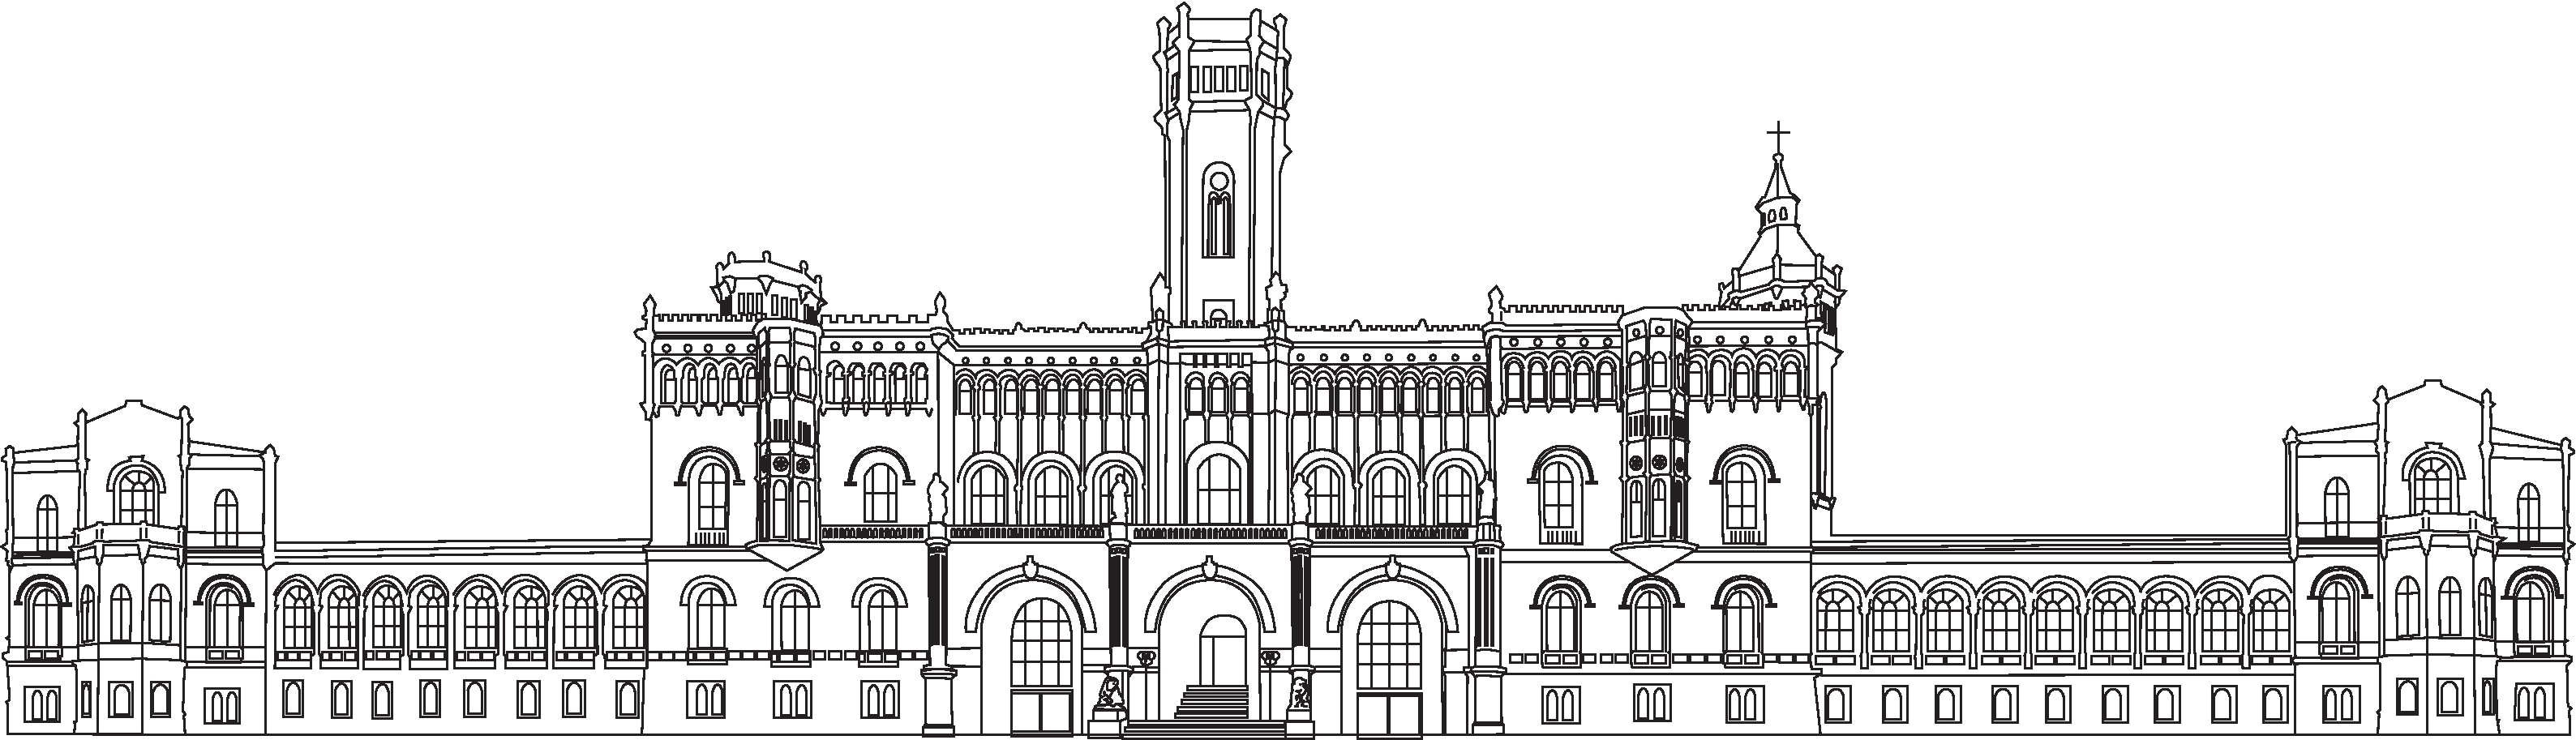
\includegraphics[width=13.8cm]{gfx/welfenschloss}
        \large  

        \hfill

        \begingroup
            %\textbf{\huge\spacedallcaps{L}\LARGE\spacedallcaps{eibniz}}
            %\textbf{\huge\spacedallcaps{U}\LARGE\spacedallcaps{niversit\"{a}t}}
            %\textbf{\huge\spacedallcaps{H}\LARGE\spacedallcaps{annover}} \\
            \huge\spacedallcaps{L}\LARGE\spacedallcaps{eibniz}
            \huge\spacedallcaps{U}\LARGE\spacedallcaps{niversit\"{a}t}
            \huge\spacedallcaps{H}\LARGE\spacedallcaps{annover} \\
        \endgroup
		\smallskip
        \normalsize
        %\spacedallcaps{\myFaculty} \\
        \myFaculty \\
        %\spacedallcaps{\myDepartment}
        \myDepartment

        \vfill
        
        %\LARGE \textbf{\myTitle} \\
        \LARGE {\color{LUHblue}\spacedallcaps Explanations for Learning-to-Rank models} \\
        \vfill
        \Large \myDegree \\
        \vfill
        
        %\large eingereicht von \\ % 		DE
        \large by \\ % 						EN
        \smallskip
        \large \spacedallcaps{Zhenye Wang} \\
        \smallskip
        %\large am \myTime \\ %				DE
        \large \myTime \\ %					EN
        
        \vfill
        
        \begin{tabular}{lll}
              %Erstpr\"{u}fer  & : & \myProf \\
              %Zweitpr\"{u}fer & : & \myOtherProf \\
			  %Betreuer        & : & \mySupervisor
              First Examiner  & :  & Prof. Dr. Avishek Anand \\
              Second Examiner & :& Prof. Dr. Wolfgang Nejdl \\
              Supervisor      & : & M.Sc. Jaspreet Singh
        \end{tabular}

        \vfill                      

    \end{center}  
  \end{addmargin}       
\end{titlepage}   

%\thispagestyle{empty}

\hfill

\vfill

\noindent\myName: \textit{\myTitle,} \mySubtitle, %\myDegree, 
\textcopyright\ \myTime

%\bigskip
%
%\noindent\spacedlowsmallcaps{Supervisors}: \\
%\myProf \\
%\myOtherProf \\ 
%\mySupervisor
%
%\medskip
%
%\noindent\spacedlowsmallcaps{Location}: \\
%\myLocation
%
%\medskip
%
%\noindent\spacedlowsmallcaps{Time Frame}: \\
%\myTime

%\cleardoublepage%*******************************************************
% Acknowledgments
%*******************************************************
\pdfbookmark[1]{Acknowledgments}{acknowledgments}



\bigskip

\begingroup
\let\clearpage\relax
\let\cleardoublepage\relax
\let\cleardoublepage\relax
\chapter*{Acknowledgments}
\textit{\centering To my supervisor: Jaspreet Singh\\ Thank you for your guidance, assistance and help. Thank you for teaching me and passing me your knowledge. Your advises and methodology gave me the opportunity to learn more and accomplish such an interesting work.\\
\centering To Prof. Avishek Anand \\ Thank you for your guidance on both academic and life, your kindness and wisdom are widely spread among students.\\
\centering To Prof. Wolfgang Nejdl \\ Thank you for leading the Research Centre, as the most highly cited computer scientist at the University of Hanover in Google Scholar is irreplaceable.\\
\centering To my mother\\ Thank you for making me the person who I am today.\\
\centering I am deeply grateful for you all.\\ }

\endgroup




%\cleardoublepage\include{FrontBackmatter/Foreword}
\cleardoublepage%*******************************************************
% Abstract
%*******************************************************
%\renewcommand{\abstractname}{Abstract}
\pdfbookmark[1]{Abstract}{Abstract}
\begingroup
\let\clearpage\relax
\let\cleardoublepage\relax
\let\cleardoublepage\relax

\chapter*{Abstract}
Learning to rank refers to machine learning techniques for training the model in a ranking task, and it is useful for many applications in Information Retrieval, Natural Language Processing, and Data Mining. But according to the current literature, as we know there are limited published papers explaining the LTR model effectively, while the models trained are often invisible to humans. Interpretabibility research on complex models is an important topic these years. For some areas such as stocks or diagnostics, we must deeply understand the internal mechanism of the model, otherwise we would rather sacrifice model performance than not be very sure of the model's decision.

In this thesis we analysis the interpretability of Learning to Rank models in a novel way. Basically, we propose a local feature attribution method that seeks to identify a small subset of input features as explanation to a ranking decision. With such subset we can recover a ranking $\pi ^{'}$, which has a very high similarity to $\pi$. In our research we defined two concepts called validity and completeness as matrics to measure the importance of features. We designed effective algorithms to seek validity and completeness of the features in subset. In general, if we list all the combinations of features, can always find the best subset as feature attribution, but for the LTR datasets with massive numbers, the number of total combinations is extremely big. Our proposed methods will greatly reduce the time cost for feature attribution. 

We tried a lot of experiments, the results reveal that with the compareation of agnostic explanation approache, which is shapley approach here. Our approach shows both accuracy and effectiveness. As a combination of validity optimized approach and completeness optimized approach, a new approach alpha, through harmonic factor $\alpha $ to make a trade of both methods is proposed, which can both optimize validity and completeness.


\vfill

%\pdfbookmark[1]{Zusammenfassung}{Zusammenfassung}
%\chapter*{Zusammenfassung}
%Kurze Zusammenfassung des Inhaltes in deutscher Sprache\dots


\endgroup			

\vfill
%\cleardoublepage%*******************************************************
% Publications
%*******************************************************
\pdfbookmark[1]{Publications}{publications}
\chapter*{Publications}
Some ideas and figures have appeared previously in the following publications:

\bigskip

\noindent Put your publications from the thesis here. The packages \texttt{multibib} or \texttt{bibtopic} etc. can be used to handle multiple different bibliographies in your document.
\cleardoublepage%*******************************************************
% Acknowledgments
%*******************************************************
\pdfbookmark[1]{Acknowledgments}{acknowledgments}



\bigskip

\begingroup
\let\clearpage\relax
\let\cleardoublepage\relax
\let\cleardoublepage\relax
\chapter*{Acknowledgments}
\textit{\centering To my supervisor: Jaspreet Singh\\ Thank you for your guidance, assistance and help. Thank you for teaching me and passing me your knowledge. Your advises and methodology gave me the opportunity to learn more and accomplish such an interesting work.\\
\centering To Prof. Avishek Anand \\ Thank you for your guidance on both academic and life, your kindness and wisdom are widely spread among students.\\
\centering To Prof. Wolfgang Nejdl \\ Thank you for leading the Research Centre, as the most highly cited computer scientist at the University of Hanover in Google Scholar is irreplaceable.\\
\centering To my mother\\ Thank you for making me the person who I am today.\\
\centering I am deeply grateful for you all.\\ }

\endgroup




\pagestyle{scrheadings}
\cleardoublepage%*******************************************************
% Table of Contents
%*******************************************************
%\phantomsection
\refstepcounter{dummy}
\pdfbookmark[1]{\contentsname}{tableofcontents}
\setcounter{tocdepth}{2} % <-- 2 includes up to subsections in the ToC
\setcounter{secnumdepth}{3} % <-- 3 numbers up to subsubsections
\manualmark
\markboth{\spacedlowsmallcaps{\contentsname}}{\spacedlowsmallcaps{\contentsname}}
\tableofcontents 
\automark[section]{chapter}
\renewcommand{\chaptermark}[1]{\markboth{\spacedlowsmallcaps{#1}}{\spacedlowsmallcaps{#1}}}
\renewcommand{\sectionmark}[1]{\markright{\thesection\enspace\spacedlowsmallcaps{#1}}}
%*******************************************************
% List of Figures and of the Tables
%*******************************************************
\clearpage

\begingroup 
    \let\clearpage\relax
    \let\cleardoublepage\relax
    \let\cleardoublepage\relax
    %*******************************************************
    % List of Figures
    %*******************************************************    
    %\phantomsection 
    \refstepcounter{dummy}
    %\addcontentsline{toc}{chapter}{\listfigurename}
    \pdfbookmark[1]{\listfigurename}{lof}
    \listoffigures

    \vspace*{8ex}

    %*******************************************************
    % List of Tables
    %*******************************************************
    %\phantomsection 
    \refstepcounter{dummy}
    %\addcontentsline{toc}{chapter}{\listtablename}
    \pdfbookmark[1]{\listtablename}{lot}
    \listoftables
        
    \vspace*{8ex}
   %\newpage
    
    %*******************************************************
    % List of Listings
    %*******************************************************      
	  %\phantomsection 
    %\refstepcounter{dummy}
    %\addcontentsline{toc}{chapter}{\lstlistlistingname}
    %\pdfbookmark[1]{\lstlistlistingname}{lol}
    %\lstlistoflistings 

    %\vspace*{8ex}
       
    %*******************************************************
    % Acronyms
    %*******************************************************
    %\phantomsection 
                     
\endgroup
\cleardoublepage
%********************************************************************
% Mainmatter
%*******************************************************
\pagenumbering{arabic}
%\setcounter{page}{90}
% use \cleardoublepage here to avoid problems with pdfbookmark
%\cleardoublepage
%\section*{Acknowledgement}
%\part{Some Kind of Manual}
 %************************************************
\chapter{Introduction}\label{ch:introduction}
%************************************************
\section{Interpretability and feature attribution}

Research on model interpretability has become a focus of attention in scientific research conferences in the past several years, because we are not only satisfied with the effect of the model, but also has more thinking about the reasons for the model decision. This kind of thinking helps to optimize the model and features, and it can help better understand the model itself and improve the quality of model services.
One of the most popular technique to achieve interpretability is to attribute the reason behind a certain decision to its input features and is called feature attribution. Feature attribution aims more specifically to characterize the response of a machine learning model by discovering which parts of the model input are most responsible for determining its output.  Feature attribution is performed post-hoc to model training in either a model introspective or model agnostic manner. Model introspective methods take model parameters and training algorithm into account whereas in the model agnostic setting only input and output is observable. Gradient based approaches for differentiable systems are a popular example here. In a model agnostic setting, feature attribution is often determined by approximating the original model by a simpler proxy model.

\section{Something missing in past literature}

Interpretability methods have recently been extended to ranking models learned from data such as click logs. This work mainly deals with textual features and ad-hoc retrieval tasks~\cite{Singhexs:2019, singh2020model, Fernando:2019:SIN:3331184.3331312}. Nevertheless, the pragmatic scenarios like web search, recommender systems, vertical search, etc operate with numerous features to work out a ranking list whereas textual features are only a a small subset. In such condition, Learning to Rank are applied, referred to as L2R or LTR for short, the core of LTR is still machine learning, but the goal is not just simple classification or regression, the most important thing is to sort the documents. While feature attribution approaches exist for standard ML models like neural networks and decision trees, they all fall under the model introspective category. In the model agnostic domain, SHAP~\cite{lundberg2017unified} and LIME~\cite{ribeiro2016i} are popular approaches devised specifically for classification and regression problems. 
However, The complexity of machine learning models makes previous papers rarely discuss that why the LTR model makes such a decision. The opacity of models becomes the bottleneck for LTR's evolution and troubleshooting. 
The feature attribution of the LTR model will first enable us to faithfully explain the output of the entire ranking, rather than explaining the score or classification results of individual items. Second, the model agnostic feature attribution method can help us cross-examine various classification algorithms without having to worry about training regimen (pointwise, pairwise, listwise), access to training data, and access to model parameters. This approach is useful not only for debugging by model developers, but also for auditing and legislative processes that strike a balance between exposing trade secrets and transparency.

\section{Thesis Goals}
The problem setting of feature attribution for LTR is as follows: given a trained model and a set of input items corresponding to a query or user, our aim is to select a subset of features, the attribution set, as an explanation that faithfully describes the ranking decision.
First, we characterize feature attributions of a given pre-trained LTR model in terms of their validity and completeness. Validity encodes the amount of predictive capacity contained in the explanatory features or attribution set. Completeness on the other hand measures the lack of information in the non-attributed set or the features that are not explanation features.
Note that an attribution set might be valid but not complete. Consider an example where the two variables encode the predictive capacity for a ranking decision and are perfectly correlated. In such a scenario, selecting any one of these variables would result in high validity. However, if only of these features is chosen into the attribution set the non-attribution set also retains enough predictive capacity. 
In this thesis we developed several categories of algorithms to explain learning to rank models, namely validity, completeness and alpha. Our methods identify a small subset of input features as explanation to a ranking decision. We have selected $\Delta$NDCG and Kendall's $\tau$ as our evaluation indicators for the explanation, namely normalized discounted cumulative gain and Kendall rank correlation coefficient, respectively.

A large number of quantitative experiments used 2 commonly LTR datasets -- MQ2008 and MSLR-WEB10K on a variety of LTR models have been set up, our experiments show that, in most cases, our feature attribution method is better than SHAP, a agnostic explanation approach, in terms of validity and completeness metrics.  

\section{Thesis Structure}
The remainder of this thesis is organized as follows: Chapter 2, provides a review of the background and the related work on both learning to rank and model explanation. Chapter 3, we make a short introduction of the features and make a more detailed definition of the problem. Chapter 4, we make a clear explanation of our novel approaches, the preference matrix and a Greedy Incremental Search algorithm were proprosed, in addition, the implement of shapley value way on explanation will also be mentioned. Within chapter 5, we present the setup of experiments, and show detailed results to analyse, we will make comparison with approached. In chapter 6 we discuss the results in depth and do more analysis, the result of alpha is revealed here. The conclusion and future enhancements are discussed in chapter 7, we summarize what we have achieved and where we need to improve.

%\cleardoublepage
%\ctparttext{}
\part{The Showcase}
%*****************************************
\chapter{Related Work}\label{ch:Related Work}
%*****************************************
\section{Review of Learning to rank Algorithms}\label{ch:Related Work1}
Learning to rank is a supervised machine learning process. For each given query-document pair, we extract features, and obtain real data annotations through log mining or manual annotation methods. Then through the rank model, the output can be similar to the real ranking list. There are three types of most used learning to rank algorithms : Pointwise, Pairwise and Listwise.
\subsection{Pointwise}
The processing object of Pointwise way is a single document. After converting the document into a feature vector, the learning system scores the document according to the classification or regression function learned from the training data. The score is the search result. Scoring formula is as follows:
\begin{equation}
\begin{aligned}
\mathrm{score} =  \mathbf w \cdot \mathbf x
\end{aligned}
\label{eqn:eq1}
\end{equation}
where  $ w $ is the weight of each dimension of the feature, and $ x $ is the feature vector converted from the doc-query. In the Ranking problem, the label of the training sample we used is not a score, but a label with a strong and weak grading, such as $Perfect> Excellent> Good> Fair> Bad$. In order to map the score to the hierarchical label, 5 thresholds need to be set. If the score falls between two adjacent thresholds, then it is divided into the corresponding label. Most common Pointwise algorithms include: PRank~\cite{crammer2002pranking}, McRank~\cite{Li:2007:MLR:2981562.2981675}, OAP-BPM~\cite{harrington2003online} and 
OPRF~\cite{Fuhr:1989:OPR:65943.65944}. In the following we make a brief introduction to PRank and McRank.

\subsubsection{PRank}
In this algorithm, the dataset can be denoted as: $X_{T\times n}$, $y$, $y\in {1, 2, 3, \dots, k}$, where $X_{T\times n}$ is features of $ T $ training samples , the feature dimension is $ n $, and the training target $ y $ has $k$ number of values.
The goal of PRank is to train a ranking rule $H$: $ R ^ n \rightarrow y$, that is, to project sample features onto $ k $ levels. 
$ H $ is defined as follows: 
\begin{equation}
\begin{aligned}
H(\mathbf x)=\min_{r \in {1, 2, 3, \dots, k}}\{r: \mathbf w \cdot \mathbf x - b_r < 0\}
\end{aligned}
\label{eqn:eq2}
\end{equation}
 Where $ w $ and $b_r, r \in {1, 2, 3, \dots, k}$ are model parameters. $\mathbf w \cdot \mathbf x$ is the score mentioned above, $ k $ number of $b_r$ is the thresholds, and $b_1 \le \dots \le b_ {k-1} \le b_k = \infty$. The main task of the PRank model is to predict these two sets of parameters $ s $ and $b_r$, $r \in {1, 2, 3, \dots, k}$, the method of updating the parameters of PRank is similar to the stochastic gradient descent , the parameters are updated every time when a sample is predicted incorrectly..

\subsubsection{McRank}
McRank is another classic Pointwise algorithm. $DCG$ (Discounted Cumulative Gain) is a indicator for evaluating the quality of a rank in the field of information retrieval. Assuming that a ranking algorithm is used to rank $ n $ documents under a specified query, you can get $DCG$ as follows:
\begin{equation}
\begin{aligned}
DCG=\sum_{i=1}^{n}c_{[\pi_i]}(2^{y_i}-1)
\end{aligned}
\label{eqn:eq3}
\end{equation}
where $ i $ represents the index order of the original document, $ c_ {[\pi_i]} = log (i + 1) $, and $ y_i $ represents the relevance level between the corresponding document and query, it is represented by $ \{0, 1, 2,3,4 \} $, 4 corresponds to a “perfect” relevance and 0 corresponds to a “poor” relevance. The larger the $DCG$ value, the better the ranking. In actual use, it is generally normalized, called $NDCG$ (Normalized discounted cumulative gain). If the $DCG$ value in descending order of gears is the highest, then the ranking problem can be turned into the prediction of document relevance categories specified by the query. That is, multi-classification problem.
For a ranking permutation mapping function $ \pi $, the $DCG$ error is $ DCG_g-DCG _ {\pi} $, where $ DCG_g $ represents the optimal sort, which is sorted in descending order according to the actual query-doc correlation, so there must be:
\begin{equation}
\begin{aligned}
DCG_g \geq DCG _ {\pi} 
\end{aligned}
\label{eqn:eq4}
\end{equation}
Suppose the training data is $\{y_i,x_i\}_i^N$, $y_i$ represents the category, then what will eventually be learned is the probability of each category $p_{i,k}=Pr(y_i=k)$, then the final sort score is:
\begin{equation}
\begin{aligned}
S_i=\sum_{k=0}^{K-1}p_i^kT(k)
\end{aligned}
\label{eqn:eq5}
\end{equation}
where $ T (k) $ represents a function which increases monotonically with the gear, and in McRank $ T (k) =  k $.

Normally the order of ranking is very important, and the Pointwise methods learn the global correlation, but does not penalize the order of the Ranking result. This is the main disadvantage of Pointwise methods.

\subsection{Pairwise}
For a search system, the system returns a list of related documents after receiving a user query, so the key to the problem is to determine the order relationship between documents. The Pointwise methods are calculated entirely from the classification score of a single document, without considering the order relationship between the documents. The Pairwise methods turn the ranking problem into a ranking problem for multiple pairs, comparing the order of different articles.
Classic Pairwise algorithms are: RankNet~\cite{Burges:2005:LRU:1102351.1102363}, RankBoost~\cite{freund2003efficient}, Ranking SVM~\cite{joachims2002optimizing}, GBRank~\cite{zheng2007regression}.
 \subsubsection{RankNet}
Suppose there is now a pair of documents $ D_i $ and $ D_j $, given a target probability $\bar{P}_{i,j}$, to indicate that document $ D_i $ will be ranked before document $ D_j $. We now express the predicted probability of $P(D_i \triangleright D_j)$ in the order of $P_{i,j}$, and define $o_i = f(x_i)$ and $o_{i,j}=f(x_i)-f(x_j)$, then we can use logistic function to represent $ P_ {i, j} $:
\begin{equation}
\begin{aligned}
P_{i,j} = \frac{e^{o_{i,j}}}{1+e^{o_{i,j}}} = \frac{1}{1+e^{-o_{i,j}}}
\end{aligned}
\label{eqn:eq6}
\end{equation}
Where $ o_{i,j} $ is the parameter to be learned. If $ D_i $  is more relevant than $ D_j $, then $P_{i,j}>0.5$, otherwise $P_{i,j}<0.5$. So the sigmoid function is used to make the probability maps to a real number on $[0, 1]$. In order to measure how close the predicted probability $P_{i,j}$ is to the target probability $\bar{P}_{i,j}$, it uses cross entropy as the loss function:
\begin{equation}
\begin{aligned}
C_{i,j} = -\bar{P}_{i,j} log P_{i,j} - (1-\bar{P}_{i,j}) log (1-P_{i,j})
\end{aligned}
\label{eqn:eq7}
\end{equation}
RankNet uses Stochastic Gradient Descent (SGD) to optimize parameters.
However, in many cases, it is not enough to evaluate the ranking based on the number of wrong pairs. Evaluation indexes in information retrieval such as $NDCG$ or $ERR$ only focus on the ranking of the top $k$ results. Because these indexes are not differentiable, RankNet cannot use them as the optimization target to iterate, so there is a gap between RankNet's optimization target and evaluation index of information retrieval.
\subsubsection{RankBoost}
RankBoost's idea is relatively simple, and it is the general idea of binary learning to rank: by constructing the target classifier, the objects in the pair have a relative size relationship. Grouping objects into pairs, such as a set of $r1> r2> r3> r4$, we can form pairs: $(r1, r2), (r1, r3), (r1, r4), (r2, r3), (r3, r4)$, if a pair is positive, then set the label to 1. The remaining pairs, such as $(r2, r1)$, should be set to -1 or 0.
The loss function is the same as defined by AdaBoost and is still defined as an exponential loss, but it is a Pairwise version:
\begin{equation}
\begin{aligned}
L(f;x_{u},x_{v},y_{u,v})=exp(-y_{u,v}(f(x_{u})-f(x_{v})))
\end{aligned}
\label{eqn:eq8}
\end{equation}
\subsubsection{Ranking SVM}
Ranking SVM is another Pairwise ranking algorithm. Given a query $q$, document $d1> d2> d3$, document $d1$ is more relevant than document $d2$, document $d2$ is more relevant than document $d3$. $x1, x2, x3$ are the characteristics of $d1, d2, d3$, respectively. In order to use machine learning for ranking, we turn the ranking problem into a classification problem. Ranking SVM defines new training samples, let $x1-x2, x1-x3, x2-x3$ be positive samples, and $x2-x1, x3-x1, x3-x2$ be negative samples, then train a binary classifier to classify these new training samples.
Ranking SVM aims to minimize the ranking loss while having a large margin, where the ranking learning step can be formulated as follows:
\begin{equation}
\begin{aligned}
& \min \limits_\mathbf{W} \ \frac{1}{2} \sum_{j=1}^{l} \| \mathbf{w}^j \|^2 + \lambda \sum_{i=1}^{n} \frac{1}{|Y_i^+||Y_i^-|} \sum_{p \in Y_i^+} \sum_{q \in Y_i^-} \xi_{pq}^i \\
		& s.t. \ \langle \mathbf{w}^p, \mathbf{x}_i \rangle - \langle \mathbf{w}^q, \mathbf{x}_i \rangle \geq 1 - \xi_{pq}^i, \ (p, q) \in Y_i^{+}  \times Y_i^{-} \\
		& \qquad \xi_{pq}^i \geq 0, \ i = 1,...,n \\ 
\end{aligned}
\label{eqn:eq9}
\end{equation}
where $Y_i^{+}$ (or $Y_i^{-}$) denotes the index set of relevant (or irrelevant) labels associated with the instance $\mathbf{x}_i$, $| \cdot |$ denotes the cardinality of a set, $\xi_{pq}^i$ is the slack variable and $\lambda$ is a tradeoff hyper-parameter which controls the model complexity. Note that it will additionally regularize the bias term $b_j$ when absorbing $b_j$ into $\mathbf{w}^j$, which is different from the original optimization problem that doesn't regularize $b_j$. Ranking SVM has good generalization ability and inherits the advantages of SVM.

But the Pairwise methods also have the following problems: 
The Pairwise method takes into account the relative order of two document pairs, but does not consider the position of the document in the list. The document ranked before the search results is more important. If the front document has a wrong judgment, the cost is significantly higher than the documents that lay behind.
At the same time, the number of related documents varies greatly from different queries, so after conversing to document pairs, some query pairs can have hundreds of corresponding document pairs, while some queries have only a dozen corresponding document pairs. So it is difficult to evaluate the effect.

\subsection{Listwise}
The Listwise methods directly consider the overall sequence and optimize the evaluation index of ranking. The most used Listwise methods are: Adarank~\cite{xu2007adarank}, SoftRank~\cite{taylor2008softrank}, LambdaRank~\cite{burges2007learning}, and LambdaMART~\cite{burges2010ranknet}.

\subsubsection{LambdaRank}
In view of the shortcoming of RankNet, LambdaRank bypasses the loss function and directly defines the gradient. First we look at the gradient of RankNet:
\begin{equation}
\begin{aligned}
\frac{\partial L}{\partial w_k} =
    \sum_{(i, j) \in P}\frac{\partial L_{ij}}{\partial w_k} =
    \sum_{(i, j) \in P}
        \frac{\partial L_{ij}}{\partial s_i}\frac{\partial s_i}{\partial w_k}
            +
        \frac{\partial L_{ij}}{\partial s_j}\frac{\partial s_j}{\partial w_k},
\end{aligned}
\label{eqn:eq10}
\end{equation}
Note the following symmetry:
\begin{equation}
\begin{aligned}
\frac{\partial L_{ij}}{\partial s_i} & {} = \frac{\partial \biggl\{\frac12 (1 - S_{ij})\sigma\cdot(s_i - s_j) + \log\Bigl\{1 + \exp\bigl(-\sigma\cdot(s_i - s_j)\bigr)\Bigr\}\biggr\}}{\partial s_i}\\
 & {}= \frac12 (1 - S_{ij})\sigma - \frac{\sigma}{1 + \exp\bigl(\sigma\cdot(s_i - s_j)\bigr)} \\
 & {}= \sigma\Biggl[\frac12(1 - S_{ij}) - \frac{1}{1 + \exp\bigl(\sigma\cdot(s_i - s_j)\bigr)}\Biggr] \\
 & {}= -\frac{\partial L_{ij}}{\partial s_j}
\end{aligned}
\label{eqn:eq11}
\end{equation}
So define:
\begin{equation}
\begin{aligned}
\lambda_{ij}\mathrel{\stackrel{\mbox{def}}{=}} \frac{\partial L_{ij}}{\partial s_i} = -\frac{\partial L_{ij}}{\partial s_j}
\end{aligned}
\label{eqn:eq12}
\end{equation}
Based on this, the gradient in LambdaRank is:
\begin{equation}
\begin{aligned}
\lambda_{ij}\mathrel{\stackrel{\mbox{def}}{=}} - \frac{\sigma}{1 + \exp\bigl(\sigma\cdot(s_i - s_j)\bigr)}\cdot\lvert\Delta Z_{ij}\rvert
\end{aligned}
\label{eqn:eq13}
\end{equation}
where  $\Delta Z$ indicates that the difference of the evaluation index (the other document orders are unchanged) obtained after exchanging the positions of the documents $D_i$ and $D_j$, from the new calculation, $\lambda_i$ is:
\begin{equation}
\begin{aligned}
\lambda_i = \sum_{j:\{i,j\} \in I} \lambda_{i,j} - \sum_{j:\{j,i\} \in I} \lambda_{i,j}
\end{aligned}
\label{eqn:eq14}
\end{equation}
This gradient represents the direction and intensity of the next iterative optimization. Due to the introduction of the IR evaluation index, Lambda gradient is more concerned about the improvement of the ranking position of high-quality documents that are positioned higher. This effectively avoids the situation of lowering the position of the high-quality document in front. The advantage of LambdaRank over RankNet is that the training speed becomes faster after factoring, and at the same time, evaluation indicators are considered.

\subsubsection{LambdaMART}
LambdaRank redefines the gradient and gives them new physical meaning. Therefore, all models that can be solved using the gradient descent can use this gradient. MART(Multiple Additive Regression Tree) is one of them. MART is an ensemble learning algorithm. Unlike the classic ensemble learning algorithm Adaboost, which uses the errors of the previous round of learners to update the sample weights of the next round of learning, MART fits the residuals generated by the previous round of classifiers each time.

Combining the gradient Lambda and MART is the famous LambdaMART algorithm. The principle of MART is to solve the function directly in the function space. The model's result consists of many trees. The fitting goal of each tree is the gradient of the loss function, in LambdaMART, it is Lambda. LambdaMART's framework is actually MART. The main innovation is that the gradients used in the intermediate calculation are Lambda and Pairwise. The parameters that MART needs to set include: the number of trees $M$, the number of leaf nodes $L$, and the learning rate $v$. These three parameters can be adjusted by the verification set to obtain the optimal parameters. 

LambdaMART has many advantages, it is more suitable for Ranking: instead of traditionally solving the ranking problem by classification or regression, but directly do ranking, and because of the tree model, you can learn different feature combinations.

\subsubsection{ListNet}
In the search scenario, all the query requests are expressed as:

$\begin{matrix} Q= \left ( q^{(1)},q^{(2)},...,q^{(m)} \right ) \end{matrix}$, for each query, there will be a search result. The results are ordered documents. For a query, the search results can be expressed as: $d^{(i)}=\left ( d_1^{(i)}, d_2^{(i)},...,d_{n^i}^{(i)}\right)$. Correspondingly, there will be a score vector representing the score of each search result: $y^{(i)}=\left ( y1^{(i)},y_2^{(i)},...,y_{n^i}^{(i)}\right )$. 
\\
Let $\pi$ represents a certain permutation, $\phi(\cdot )$ is a monotonically increasing function with a positive range. For a certain permutation and its score, the probability of defining the current permutation is:
\begin{equation}
\begin{aligned}
P_s(\pi)=\prod_j^n \frac{\phi(s_{\pi(j)})}{\sum_{k=j}^n \phi(s_{\pi(k)})}
\end{aligned}
\label{eqn:eq15}
\end{equation}
where $s_{\pi(j)}$ is the score of object at position $j$ of permutation $\pi$. The top one probability of object $j$
is defined as:
\begin{equation}
\begin{aligned}
P_s(j) = \frac{\phi(s_j)}{\sum_{k=1}^n \phi(s_k)}
\end{aligned}
\label{eqn:eq16}
\end{equation}
The cross entropy loss function:
\begin{equation}
\begin{aligned}
L(y^{(i)}, z^{(i)}) = - \sum_{j=1}^{n^{(i)}} P_{y^{(i)}}(j) \log P_{z^{(i)}}(j) = - \sum_{j=1}^{n^{(i)}} \frac{\phi(y_j^{(i)})}{\sum_{k=1}^n \phi(y_k^{(i)})} \log \frac{\phi(z_j^{(i)})}{\sum_{k=1}^n \phi(z_k^{(i)})}\end{aligned}
\label{eqn:eq16}
\end{equation}
where $y$ is the actual label and $z$ is the prediction.
ListNet's model is a neural network, it has proven to be a better method than Pairwise. Of course, the complexity of fitting its parameters is also much higher than others.

\newpage
\section{Review of Model Interpretability}
Machine learning business applications target output decision making. Interpretability refers to the degree to which humans can understand the reason for a decision. The more interpretable a machine learning model is, the easier it is for people to understand why certain decisions or predictions are made. Model interpretability refers to the understanding of the internal mechanism of the model and the results of the model. It‘s importance is reflected in: the modeling phase, assisting developers to understand the model, comparing and selecting models, and optimizing models. In the operational phase, explaining the internal mechanism of the model to the business party and explaining the model results. For example, a fund recommendation model needs to explain: why a certain fund is recommended for this user or not.

\paragraph{Model Improvement}
Understanding the characteristics of indicators, classification, and predictions, and then why a machine learning model makes such a decision, and which features play the most important role in the decision, allows us to judge whether the model is consistent with common sense. Knowing how the model uses features to make predictions, we can intuitively determine whether our model captures meaningful features and whether the model can be generalized to the predictions of other samples.

\paragraph{Model Credibility and Transparency}
Understanding machine learning models is necessary to improve the credibility of the model and to provide transparency in reviewing and predicting the results. It is unrealistic for black box models to determine people's lives, such as loans and prison criminal law. Another area that questions the credibility of machine learning results is medicine, and model results directly determine the life and death of patients. Machine learning models are very accurate in distinguishing malignant tumors from different types of benign tumors, but we still need experts to explain the diagnosis and explain why a machine learning model will classify a patient's tumor as benign or malignant and help doctors trust and use machine learning models to support their work.
\paragraph{Prevent Biases}
Biased models are often caused by biased samples. If the data contains subtle biases, the model learns and thinks the fit is good. A well-known example is the use of machine learning models to suggest convictions and sentencing for prisoners, which clearly reflects the inherent bias of the justice system over racial inequality. Other examples include machine learning models for recruitment that reveal gender bias in specific positions, such as male software engineers and female nurses.

~\\
The explaination attempts to understand and explain these decisions made by the response function, namely, what, why, and how. The key to model interpretation is transparency, the ability to question, and the ease with which humans understand model decisions. The three most important aspects of model interpretation are explained below:
\paragraph{What drives the model's predictions?}
 We should be able to query our model and identify potential feature interactions to understand which features may be important in the model's decision strategy. This ensures the fairness of the model.
\paragraph{Why does the model make a decision?}
We should also be able to verify and justify why certain key features are responsible for driving certain decisions made by the model during the forecast period. This ensures the reliability of the model.
\paragraph{How do we trust model predictions?}
We should be able to evaluate and validate any data point and how the model makes decisions about it. This should be provable and easy to understand for the key stakeholders where the model works as expected. This ensures the transparency of the model.

\subsection{Interpretable Model}
Among the algorithms for machine learning, some models are difficult to interpret, such as deep neural networks. Deep neural networks can fit highly complex data with huge parameters, but how to interpret these is very difficult. However, there are still quite a few algorithms that can be easily explained.

For example, linear regression. Linear regression is easy to use and can also guarantee to find the optimal solution. But not all problems are linear after all. Another example of an interpretable model is decision tree. The decision tree clearly gives the basis for prediction. To explain how a decision tree predicts is very simple, it starts from the root node, starts branching according to all features, and reaches the leaf node to find the final prediction.

Decision trees can well capture the interactions and dependencies between features. The tree structure can also be well visualized. However, the decision tree is difficult to handle the linear relationship. It is not smooth and unstable, and a small change in feature data may change the construction of the entire tree. As the nodes and levels of the tree become larger, it becomes more difficult to explain the entire decision-making process. There are much other interpretable models, such as logistic regression, general linear models, Naive Bayes, Kmeans, etc.


\subsection{Model-agnostic Methods}
After all, the types of interpretable models are limited, and we hope to find some ways to provide explanations for any black box machine learning model. Here we need a model-agnostic methods.
\subsubsection{Partial Dependence Plot (PDP)}
PDP is used to represent the impact of one or two features in a model on the prediction. The PDP chart below shows three characteristics of temperature, humidity, and wind speed on the number of cyclists. Each graph is a trend assuming that other features are constant.

\begin{figure}[H]
\centering
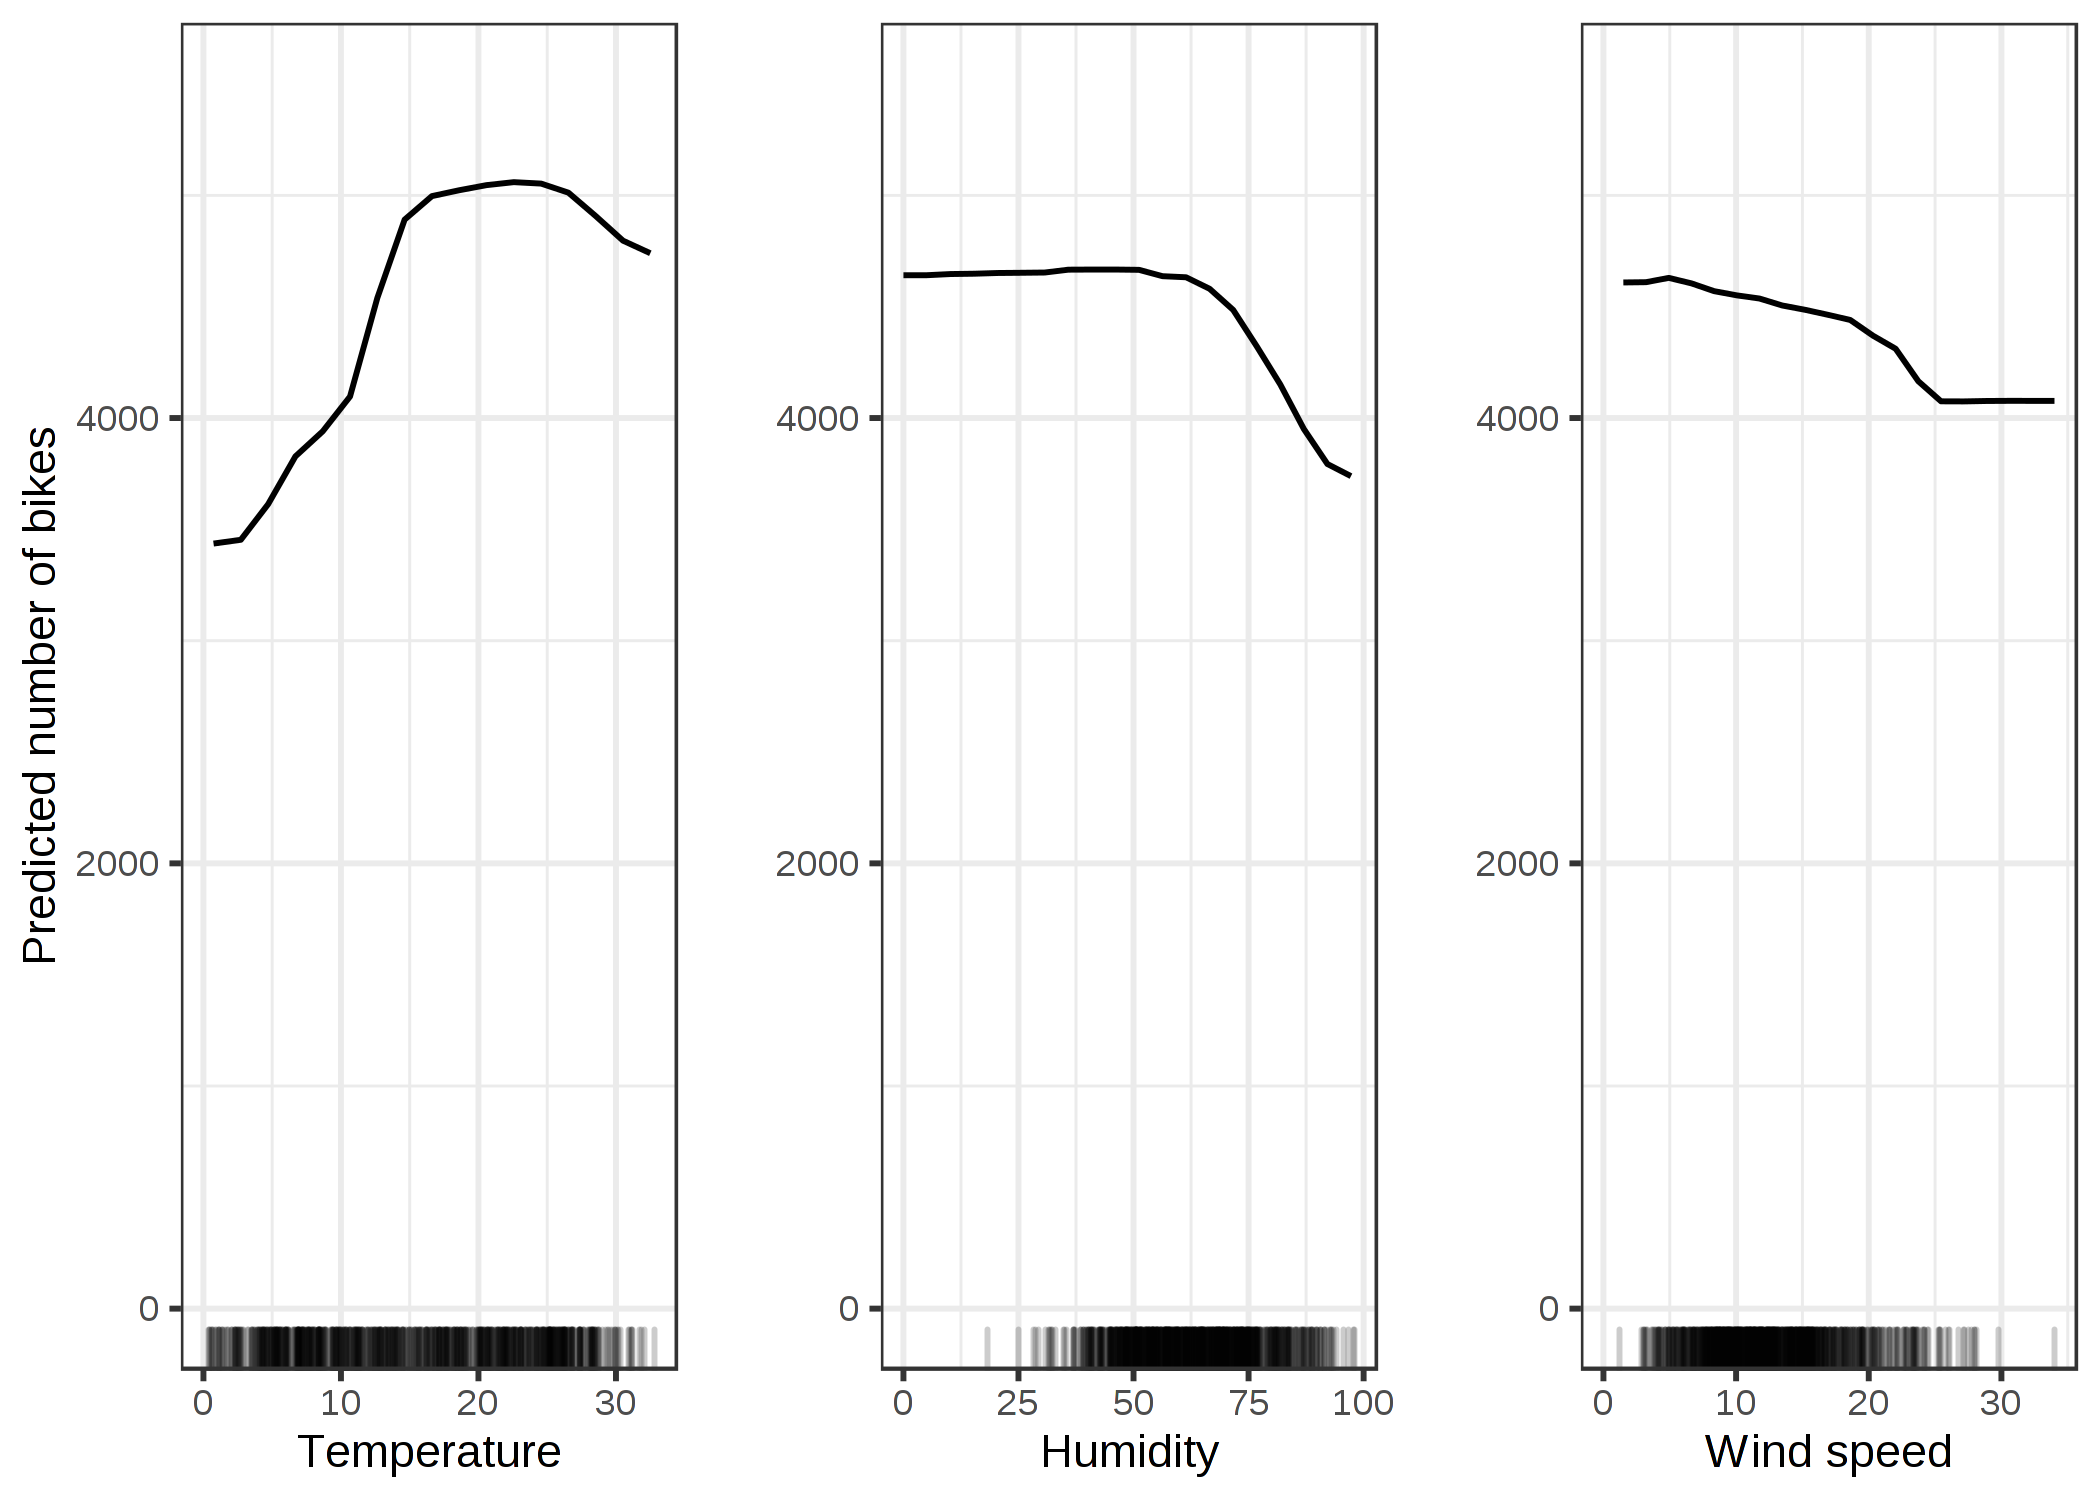
\includegraphics[width=0.6\columnwidth]{gfx/pdp-bike-1.png}
\caption{PDPs for the bicycle count prediction model and temperature, humidity and wind speed.~\cite{molnar2019}}
\label{fig:pdp-bike}
\end{figure}

PDP diagrams are very intuitive and easy to calculate and generate. However, PDP maps can only reflect two features at most, because more than three-dimensional maps cannot be represented by current technology. At the same time, the independence assumption is the biggest problem of PDP.

\subsubsection{Individual Conditional Expectation (ICE)}
The ICE and PDP charts reflect a consistent trend, but include all samples. Similar to PDP, ICE's independence assumption and inability to characterize more than two features are it's limitations. At the same time, as the number of samples increases, the graph will become quite crowded.
\begin{figure}[H]
\centering
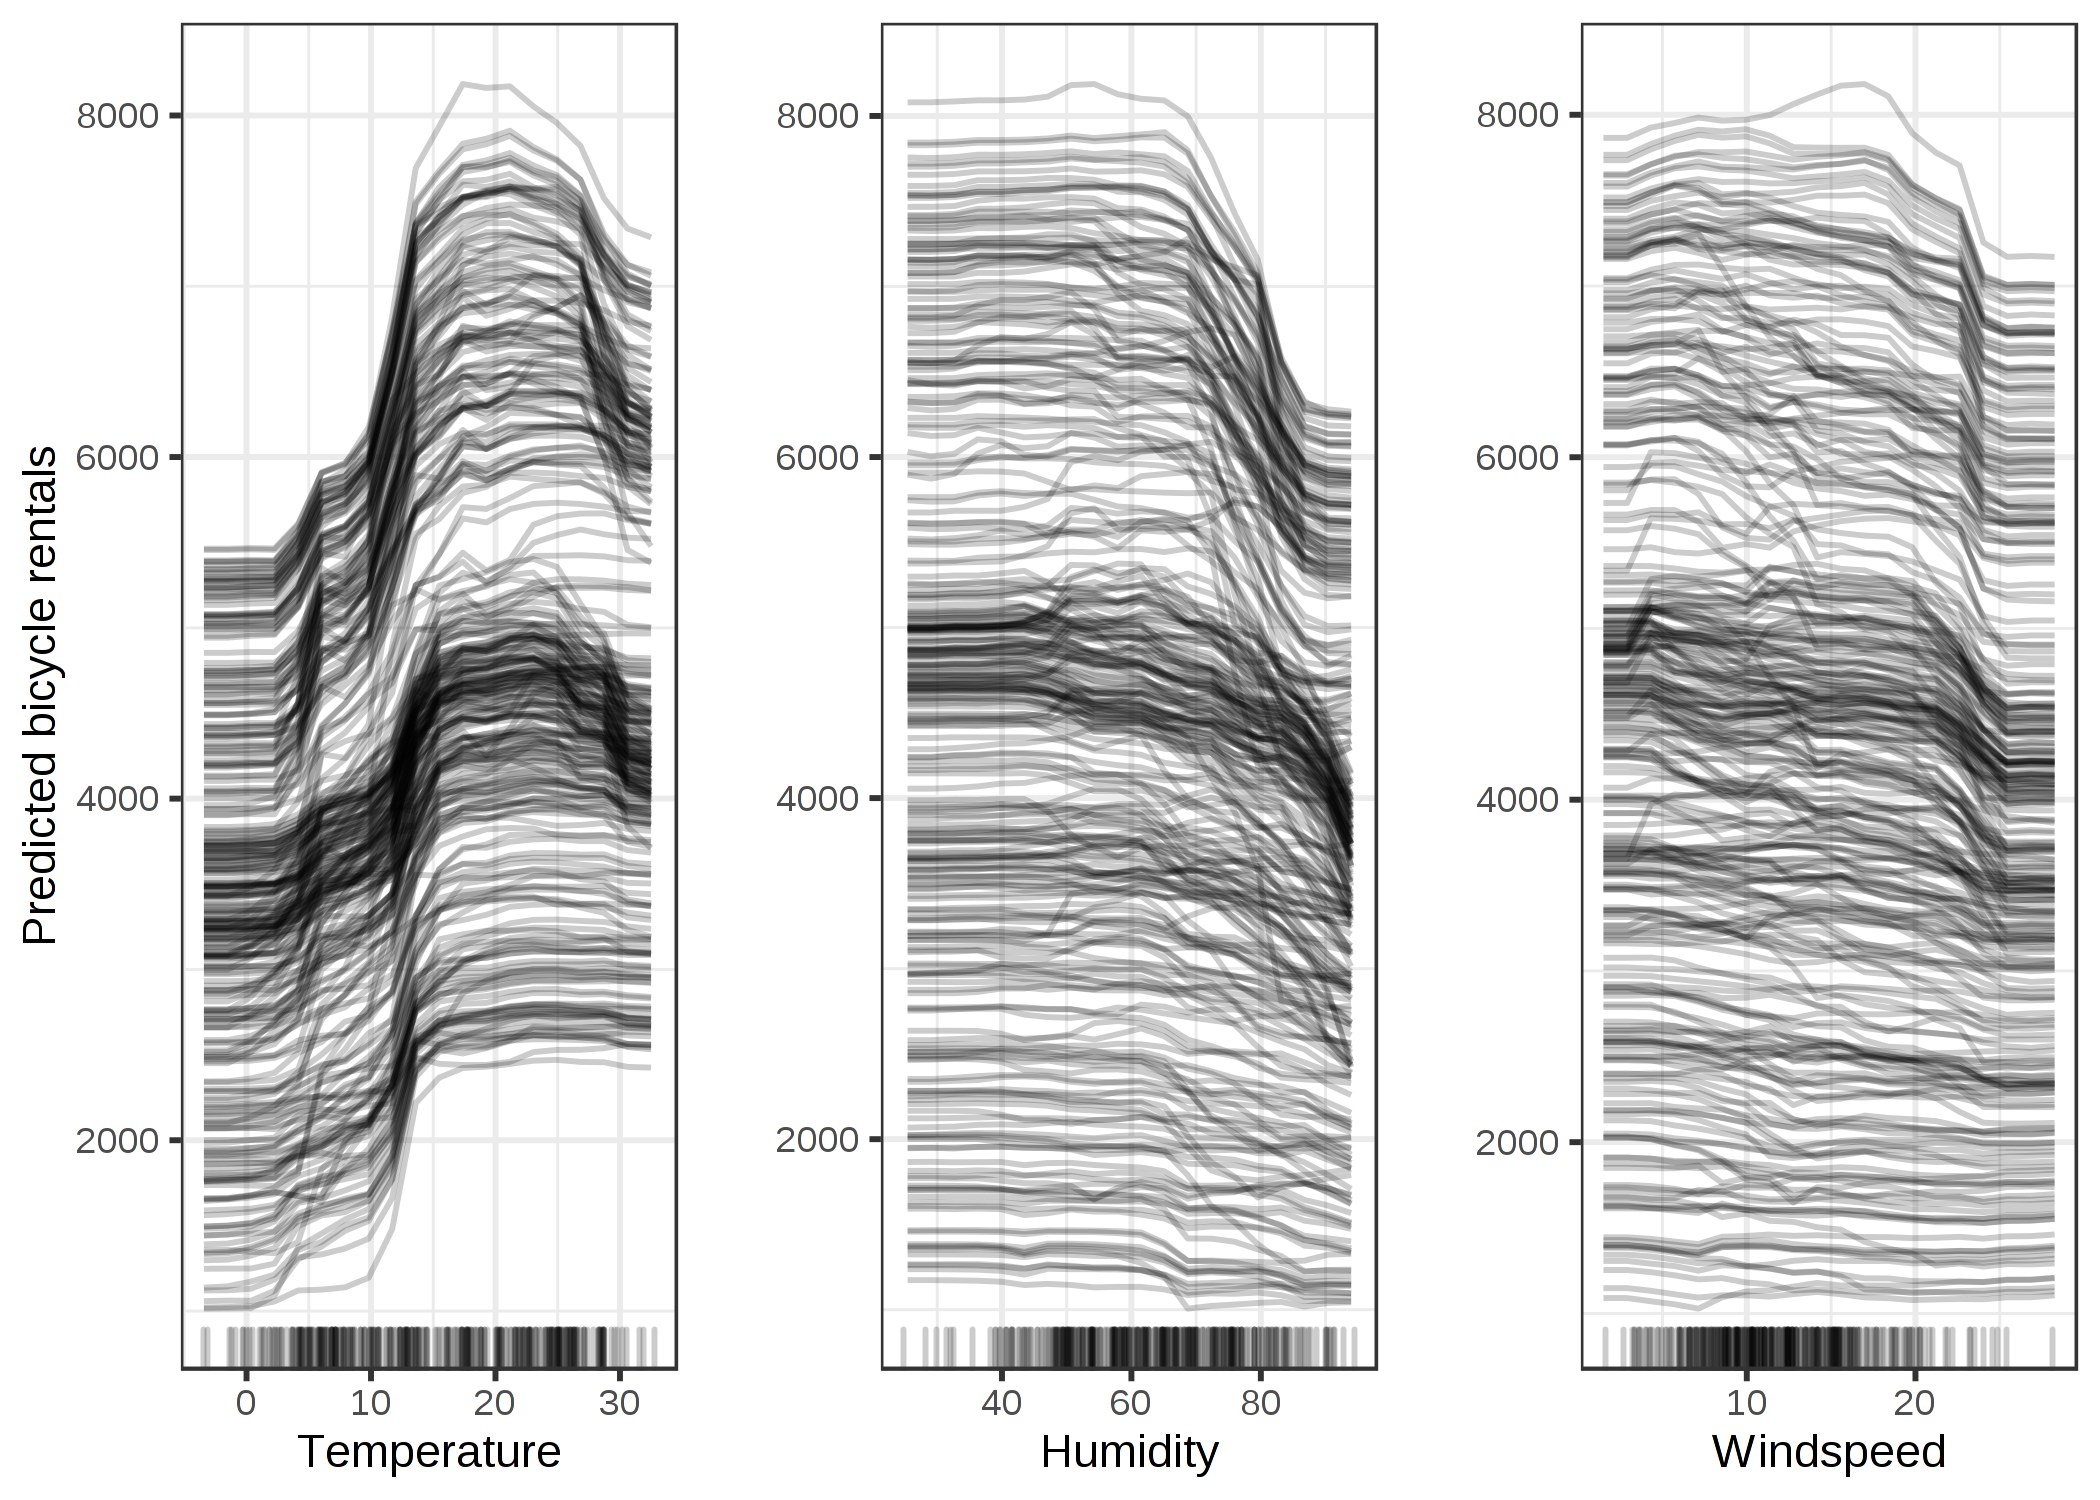
\includegraphics[width=0.6\columnwidth]{gfx/ice-bike-1.png}
\caption{ ICE plots of predicted bicycle rentals by weather conditions.~\cite{molnar2019}}
\label{fig:ice-bike}
\end{figure}

\subsubsection{Feature Interaction}
For example, a model has two features, then the model can be a constant and a term containing only the first feature and a term containing only the second feature and an interaction term between the two features. 
\begin{figure}[H]
\centering
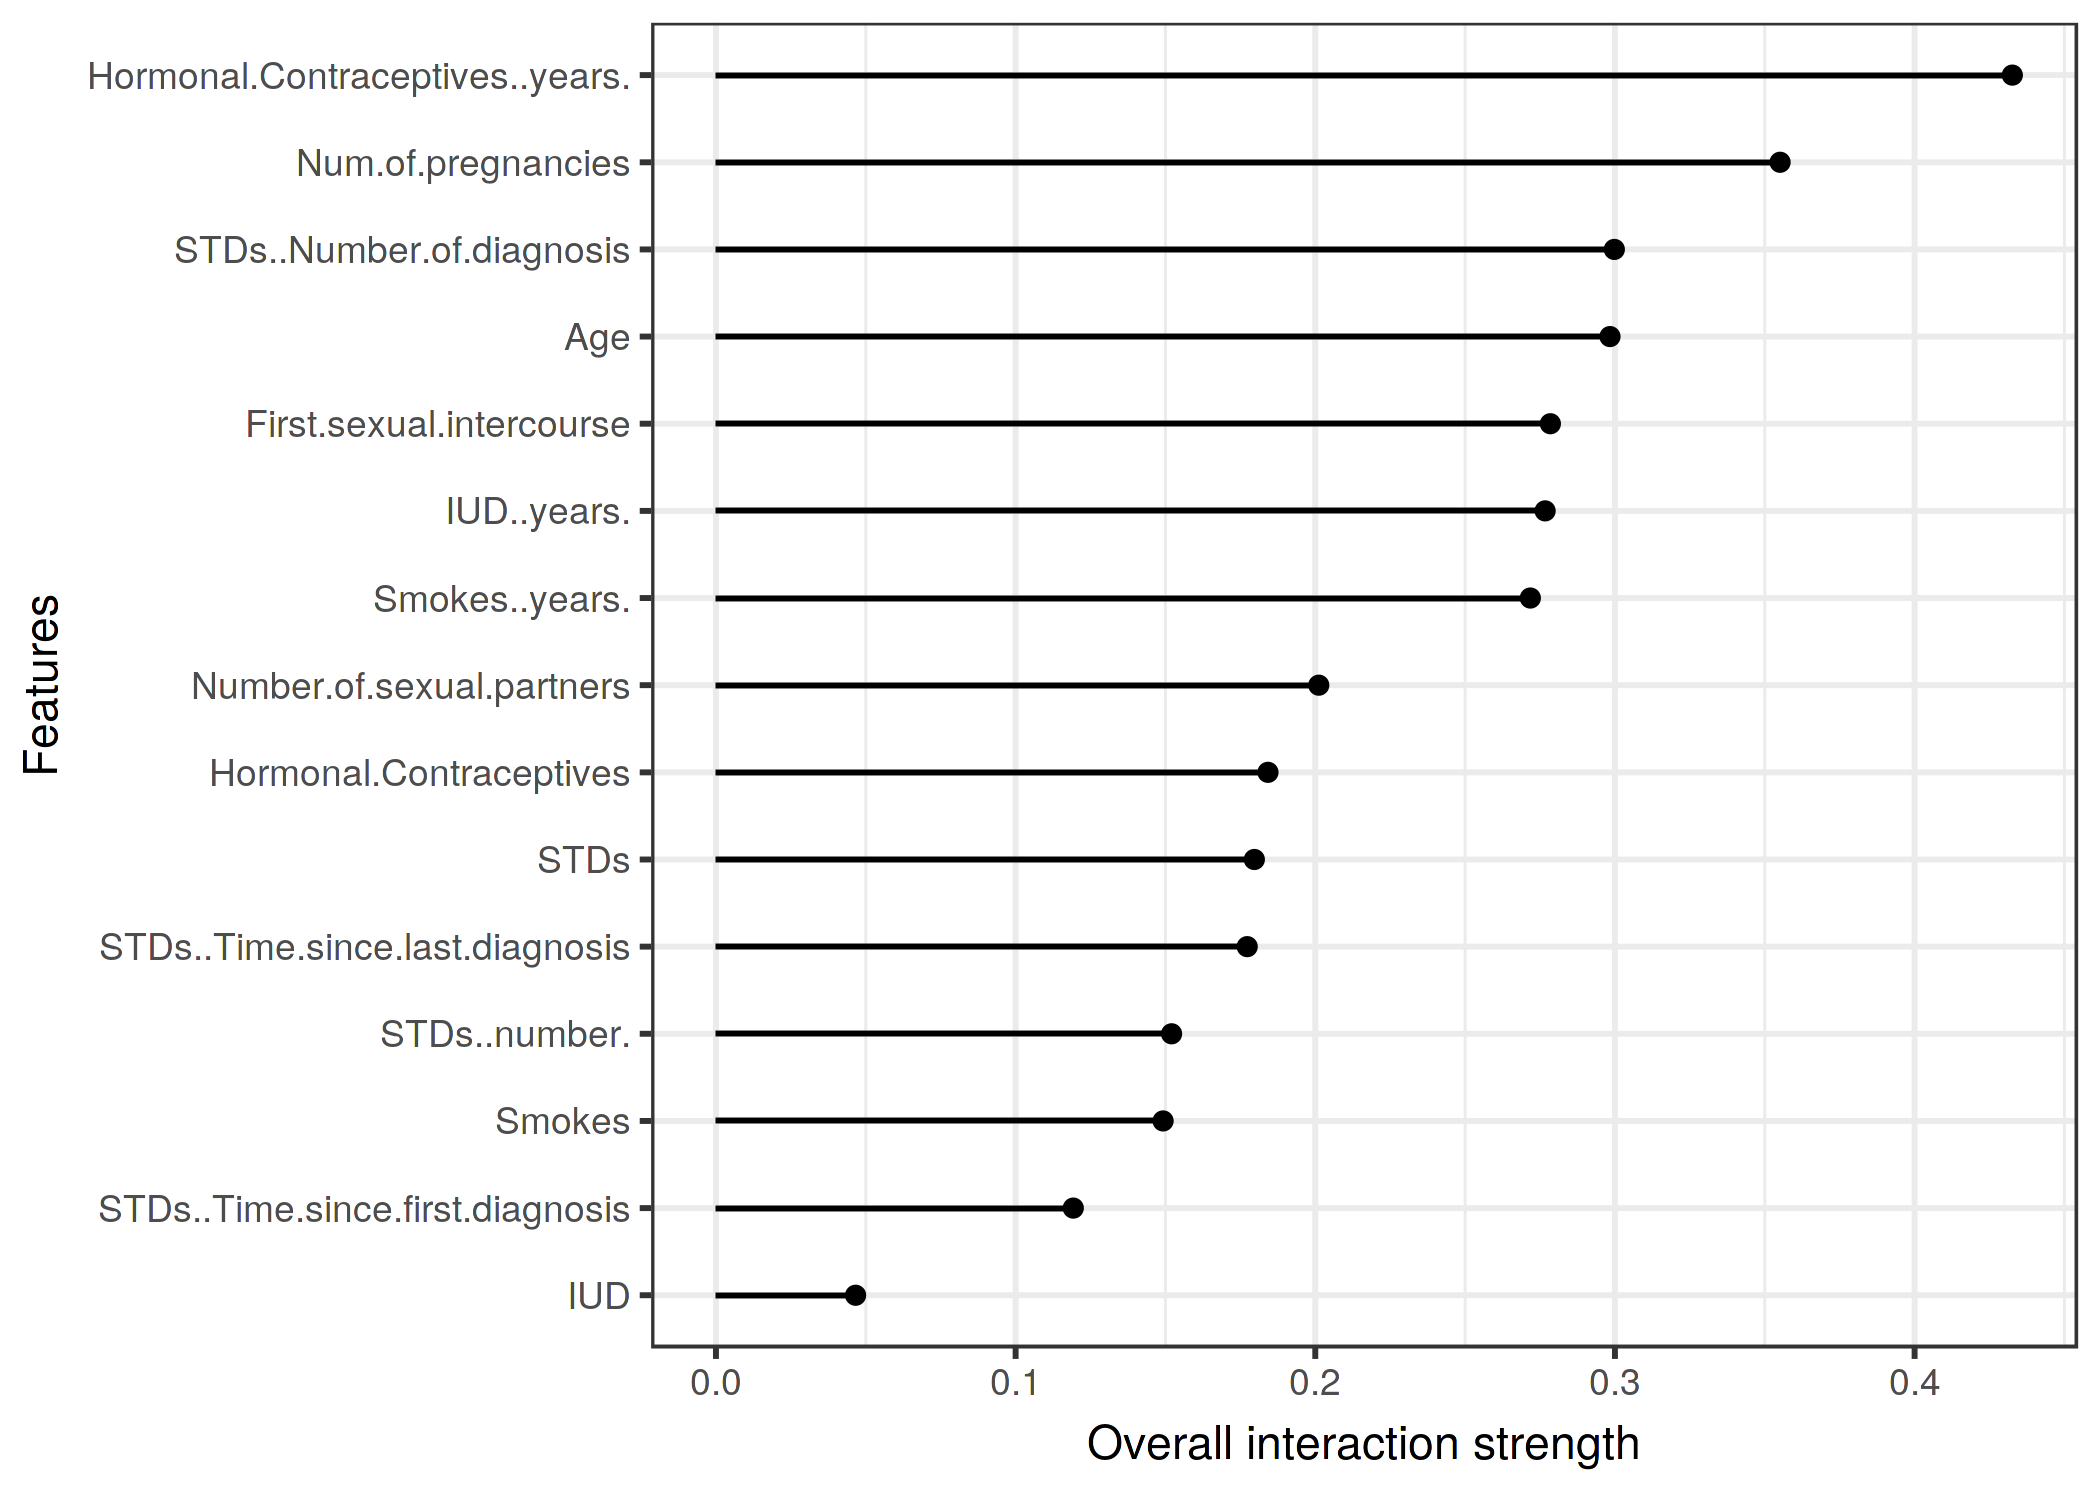
\includegraphics[width=0.6\columnwidth]{gfx/interaction-cervical-1.png}
\caption{The interaction strength (H-statistic) for each feature with all other features for a support vector machine predicting bicycle rentals.~\cite{molnar2019}}
\label{fig:interaction}
\end{figure}
~\\Using Friedman's H-statistic theory, we can calculate feature interactions. H-statistic calculations are resource-intensive and the results are not very stable.

\subsubsection{Feature Importance}
The definition of feature importance is the change caused by the prediction error when the value of a feature is changed. When we change a feature, the prediction error changes greatly, indicating that the feature has a great influence. On the contrary, if the value of another feature is changed, it has no effect on the error of the prediction result. It doesn't matter.
\begin{figure}[H]
\centering
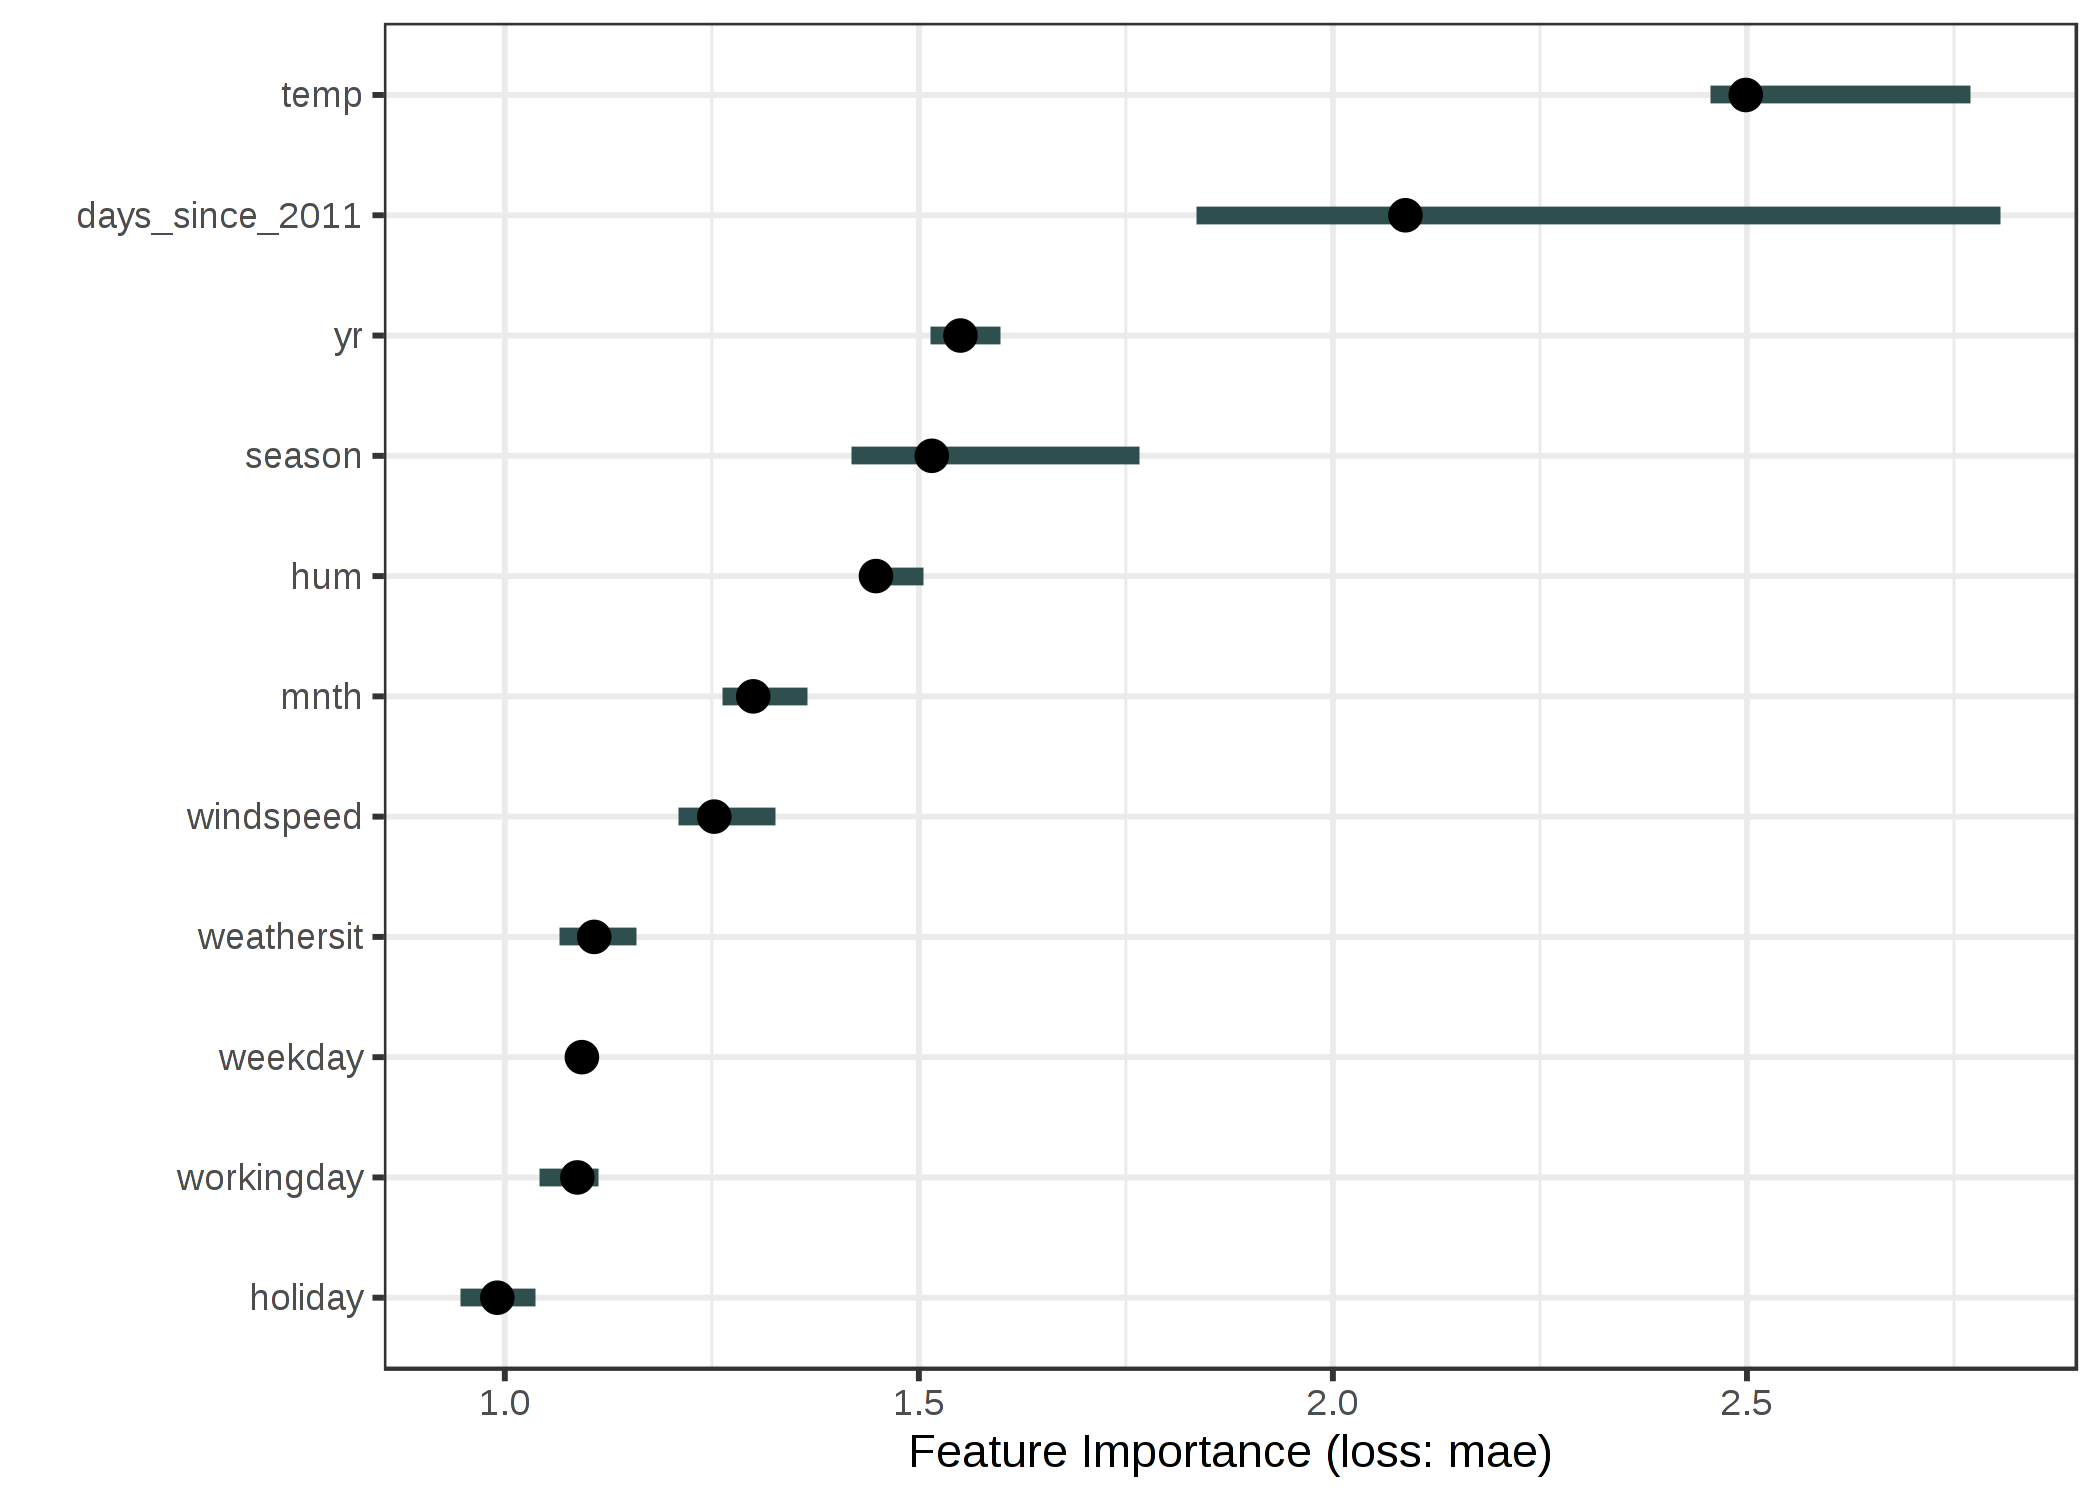
\includegraphics[width=0.6\columnwidth]{gfx/importance-bike-1.png}
\caption{The importance for each of the features in predicting bike counts with a support vector machine.~\cite{molnar2019}}
\label{fig:importance}
\end{figure}

\subsubsection{Surrogate Model}
The substitute model is a simpler model that can be interpreted. For the input and prediction of the black box model, a substitute is trained. This model is used to explain the complex black box model.
The training processes of the alternative model are as follows:
\\\\1. Choose a data set X (can be the same or different from the training set)
\\\\2. Predicting Y with a trained black box model.
\\\\3. Choose an interpretable model, such as a linear regression or decision tree.
\\\\4. Train this interpretable model with the previous dataset X and prediction Y.
Verify the differences between explainable models and black box models. Alternative models are flexible, intuitive and easy to implement,but it is an interpretation of the black box model, not an interpretation of the data.

\subsubsection{LIME}
What is LIME? Which is a local interprentable model-agnostic explanation proposed by Ribeiro in 2016~\cite{ribeiro2016i}. They use $G$ to represent models that may be used for interpretation, it can be a linear model, a tree model or a simple set of rules, use $g \in G$ to represent a specific interpretive model, that is, $g$ is a model trained on $x^{\prime} \in \lbrace 0,1 \rbrace ^{d^\prime}$. For the interpretability of the model, the model cannot be too complicated. Therefore, we use $\Omega(g)$ to represent the complexity of the model. We need to limit the complexity of the model to a certain range. In addition, the $g$ that we use to explain the model should be as close to $f$ as possible, at least to maintain the authenticity around the sample $x$ that needs to be explained. The way we use to define the surrounding is $\pi_x(z)$, in fact, it indicates how far away $z$ is from the sample $x$, the closer, the greater the weight should be. So the explaination of the model is:
\begin{equation}
\begin{aligned}
\xi(x) = \mathop {argmin}_{g\in G} L(f, g, \pi_x) + \Omega(g)
\end{aligned}
\label{eqn:eq1}
\end{equation}
The explaination of the sample $x$ is to find a interpretable model that is most similar in the local part of $x$ and has the lowest complexity.

\begin{figure}[H]
\centering
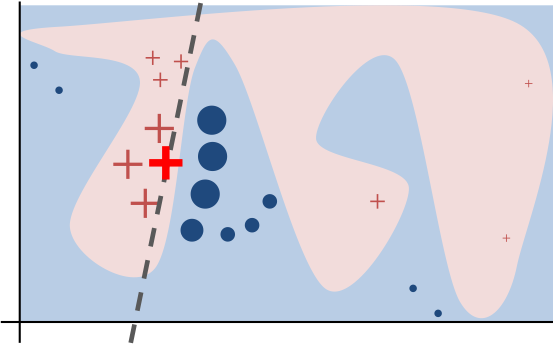
\includegraphics[width=0.5\columnwidth]{master_thesis/gfx/lime.png}
\caption{Toy example to present intuition for LIME. Figure from~\cite{ribeiro2016i}}
\label{fig:lime}
\end{figure}

~\\$G$ is expressed using a linear model: $g(z^\prime) = w_g g^\prime$, and $\pi_x(z) = exp(-D(x, z)^2/\sigma^2)$, so $L(f,g,\pi_x)=\sum_{z,z^\prime \in Z}\pi_x(z)(f(z) - g(z^\prime))^2$.
For this kind of linear model, when the model to be explained is very complicated, or when it is locally non-linear, it is not good to use a linear model to explain it. In addition, if the input itself cannot be broken into parts and uses missing or existing to affect the output, there is no way to use this method to explain.
\subsubsection{Anchor}
Anchor~\cite{ribeiro2018anchors} proposed in a paper by Reberio on AAAI in October 2018, a continuation of LIME. Anchors explains individual predictions of any black-box classification model by finding a decision rule that anchors the prediction sufficiently. Like its predecessor, the anchors approach deploys a perturbation-based strategy to generate local explanations for predictions of black-box machine learning models. However, instead of surrogate models used by LIME, the resulting explanations are expressed as easy-to-understand IF-THEN rules, called anchors. These rules are reusable since they are scoped: anchors include the notion of coverage, stating precisely to which other possibly unseen instances they apply. 
An anchor $A$ is formally defined as follows:
\begin{equation}
\begin{aligned}
\mathbb{E}_{\mathcal{D}_x(z|A)}[1_{f(x)=f(z)}]\geq\tau,A(x)=1
\end{aligned}
\label{eqn:eq2}
\end{equation}
where $A$ is a set of predicates, i.e., the resulting rule or anchor, $D_x (\cdot|A)$ indicates the distribution of neighbors of $x$, $0 \leq \tau \leq 1$ specifies a precision threshold. Given an instance $x$ to be explained, a rule or an anchor $A$ is to be found, such that it applies to $x$, while the same class as for $x$ gets predicted for a fraction of at least $\tau$ of $x$'s neighbors where the same $A$ is applicable. $A$ rule's precision results from evaluating neighbors or perturbations (following $D_x (z|A)$) using the provided machine learning model (denoted by the indicator function $1_{f(x) = f(z)}$).
\begin{figure}[H]
\centering
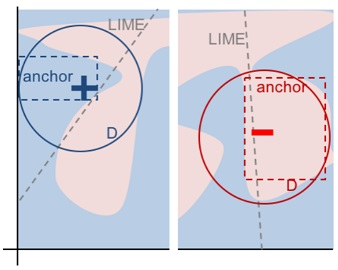
\includegraphics[width=0.5\columnwidth]{gfx/anchors-visualization.jpg}
\caption{LIME vs. Anchors. Figure from ~\cite{ribeiro2018anchors}}
\label{fig:Anchors}
\end{figure}

\subsubsection{Shapley Values}
Lundberg's 2017 approach to explain models through the SHAP\\ method~\cite{lundberg2017unified}. The main idea of the SHAP method is the shapley value. The Shapley value is a method derived from cooperative game theory. The Shapley value created by Shapley in 1953 is a method of allocating expenses to players based on their contribution to the total expenditure. Players cooperate in the alliance and get a certain benefit from this cooperation. If you use the value to explain the prediction of machine learning, "Total Expenditure" is the model prediction value of a single instance of the data set, "Player" is the characteristic value of the instance, and "Return" is the actual prediction of the instance minus the average of all instances prediction.
We are interested in how each feature affects the prediction. It is easy to calculate the contribution of each feature in a linear model. Here is what a linear model prediction looks like for one data instance:
\begin{equation}
\begin{aligned}
\hat{f}(x)=\beta_0+\beta_{1}x_{1}+\ldots+\beta_{p}x_{p}
\end{aligned}
\label{eqn:eq3}
\end{equation}
where $x$ is the instance for which we want to compute the contributions. Each $x_j$ is a feature value, with $j = 1,...,p$. The $\beta_j$ is the weight corresponding to feature $j$.
The contribution $\phi_j$ of the j-th feature on the prediction $\hat{f}(x)$ is:
\begin{equation}
\begin{aligned}
\phi_j(\hat{f})=\beta_{j}x_j-E(\beta_{j}X_{j})=\beta_{j}x_j-\beta_{j}E(X_{j})
\end{aligned}
\label{eqn:eq4}
\end{equation}
The shapley value of a feature value is its contribution to the payout, weighted and summed over all possible feature value combinations:
\begin{equation}
\begin{aligned}
\phi_j(val)=\sum_{S\subseteq\{x_{1},\ldots,x_{p}\}\setminus\{x_j\}}\frac{|S|!\left(p-|S|-1\right)!}{p!}\left(val\left(S\cup\{x_j\}\right)-val(S)\right)
\end{aligned}
\label{eqn:eq5}
\end{equation}
where $S$ is a subset of the features used in the model, $x$ is the vector of feature values of the instance to be explained and p the number of features. $val_x(S)$ is the prediction for feature values in set $S$.
First, select an instance of interest $x$, a feature $j$ and the number of iterations $M$. For each iteration, a random instance $z$ is selected from the data and a random order of the features is generated. Two new instances are created by combining values from the instance of interest $x$ and the sample $z$. The first instance $x_{+j}$ is the instance of interest, but all values in the order before and including value of feature $j$ are replaced by feature values from the sample $z$. The second instance $x_{-j}$ is similar,it has all the values in the order before, but excluding feature $j$ replaced by values of feature $j$ from the sample $z$. The difference in the prediction from the black box is computed:
\begin{equation}
\begin{aligned}
\phi_j^{m}=\hat{f}(x^m_{+j})-\hat{f}(x^m_{-j})
\end{aligned}
\label{eqn:eq6}
\end{equation}
All these differences are averaged and result in:
\begin{equation}
\begin{aligned}
\phi_j(x)=\frac{1}{M}\sum_{m=1}^M\phi_j^{m}
\end{aligned}
\label{eqn:eq7}
\end{equation}
Averaging implicitly weighs samples by the probability distribution of $X$. The procedure has to be repeated for each of the features to get all shapley values.

Like many other permutation-based interpretation methods, the shapley value method suffers from inclusion of unrealistic data instances when features are correlated. 

\subsection{Example-Based Methods}

\subsubsection{Adversarial}
The adversarial sample refers to the fact that when a small change is made to a certain feature value of a sample, the entire model makes a wrong prediction, this concept was proposed in Szegedy~\cite{szegedy2013intriguing}. The goal of adversarial samples is to deceive models, and the means by which hackers attack machine learning models is often to find these adversarial examples.
\begin{figure}[H]
\centering
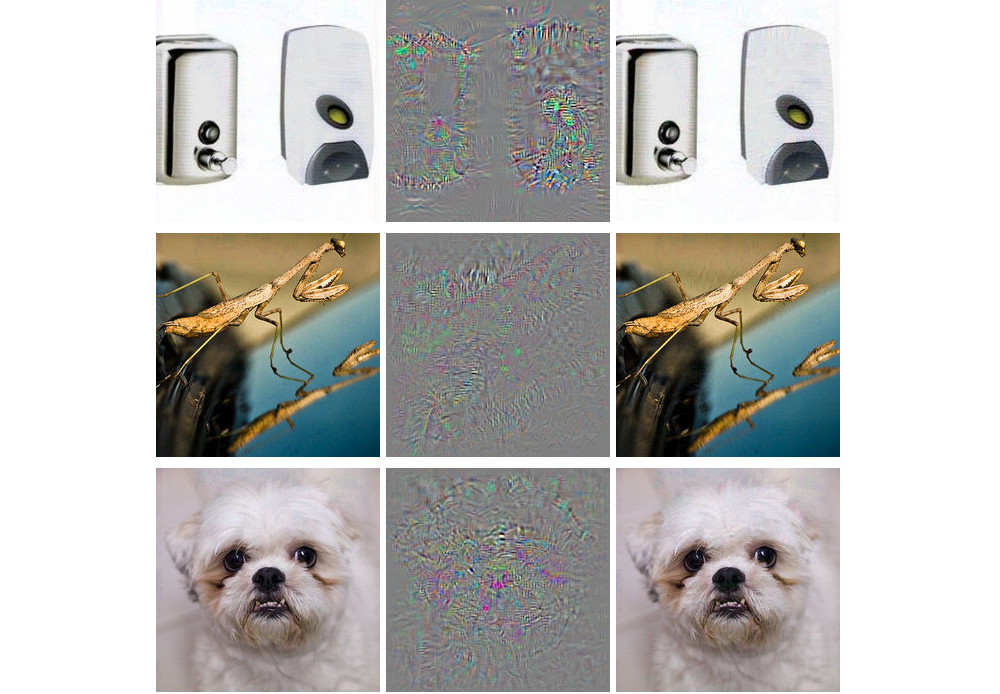
\includegraphics[width=0.5\columnwidth]{gfx/adversarial-ostrich.jpg}
\caption{Adversarial examples for AlexNet from ~\cite{szegedy2013intriguing}}
\label{fig:Adversarial}
\end{figure}
~\\These adversarial examples were generated by minimizing the following function:
\begin{equation}
\begin{aligned}
loss(\hat{f}(x+r),l)+c\cdot|r|
\end{aligned}
\label{eqn:eq8}
\end{equation}
~\\where x is an image, r is the changes, l is the desired outcome class, and the parameter c is used to balance the distance between images and the distance between predictions. 
\\\\Zhao~\cite{zhao2017generating} proposed a method to generate more natural, legible adversarial samples, which can be used to measure the robustness of the model. The steps are as follows:
\\\\1. Train a generator $G_{\theta}:Z\to X$ using WGAN~\cite{arjovsky2017wasserstein} and (unlabeled) real data X.
\\\\2. Train its inverse function $I_{\gamma}:X\to Z$ according to the generator.The specific training way is as follows:
\begin{equation}
\begin{aligned}
\underset{\gamma}{\mathrm{min}} \quad E_{x\sim p(x)}(\lVert G_\theta(I_\gamma(x)) - x\rVert) + \lambda\cdot E_{z\sim p(z)}(L(z,I_\gamma(G_\theta(z))))
\end{aligned}
\label{eqn:eq10}
\end{equation}
\\\\3. For a specific real data $x$, use $I_{\gamma}$ to map it back to the hidden space, that is, $z'=I_\gamma(x)$, and then randomly perturb $z'$ on the hidden space to get $\tilde{z}$, and finally $\tilde{x}=G_\theta(\tilde{z})$ gets the corresponding adversarial sample.
\\\\The adversarial samples generated based on this method will be more natural in appearance.

\subsubsection{Counterfactual}
The counterfactual explanation is like saying "If X didn't happen, Y wouldn't happen".
\begin{figure}[H]
\centering
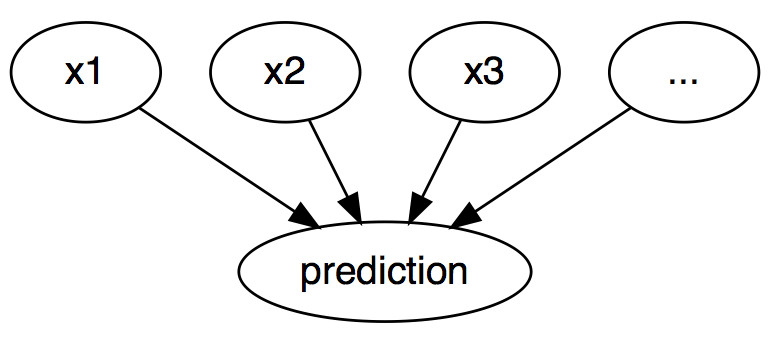
\includegraphics[width=0.5\columnwidth]{gfx/counterfactual.jpg}
\caption{The causal relationships between inputs of a machine learning model and the predictions.Figure from ~\cite{molnar2019}}
\label{fig:counterfactual}
\end{figure}
~\\We do this by changing a feature of a sample and then observing the change in the prediction result. Google's what if tool~\cite{wexler2019whatif} can help us do this analysis.



%************************************************
\chapter{Problem Defination}\label{ch:Problem Defination} % $\mathbb{ZNR}$
%************************************************
\subsection{Learning to Rank Features}
For a learning to rank task, the model handles features to make a rank list. For each query-document pair, it contains host of features, for instance, for dataset MQ2008 from LETOR 4.0~\cite{qin2013introducing}, which is a Supervised ranking dataset. Here are several example rows from MQ2008 dataset: 

\begin{lstlisting}
2 qid:10032 1:0.056537 2:0.000000 3:0.666667 4:1.000000 5:0.067138 ... 45:0.000000 46:0.076923 #docid = GX029-35-5894638 inc = 0.0119881192468859 prob = 0.139842 
0 qid:10032 1:0.279152 2:0.000000 3:0.000000 4:0.000000 5:0.279152 ... 45:0.250000 46:1.000000 #docid = GX030-77-6315042 inc = 1 prob = 0.341364 0 qid:10032 1:0.130742 2:0.000000 3:0.333333 4:0.000000 5:0.134276 ... 45:0.750000 46:1.000000 #docid = GX140-98-13566007 inc = 1 prob = 0.0701303 
1 qid:10032 1:0.593640 2:1.000000 3:0.000000 4:0.000000 5:0.600707 ... 45:0.500000 46:0.000000 #docid = GX256-43-0740276 inc = 0.0136292023050293 prob = 0.400738 

\end{lstlisting}
Each row represents a query-document pair. The first column is relevance label of this pair, the second column is query id, the following columns are features, and the end of the row is comment about the pair, including id of the document. The larger the relevance label, the more relevant the query-document pair. A query-document pair is represented by a 46-dimensional feature vector, they are show in table~\ref{tab:features}. Some features like the second one TF of anchor, the 39th LMIR.JM of URL, the 41th PageRank score, in common sense, they are important features. 
\begin{longtable}{|c|l|}
\hline
Column in Output & Description                             \\ \hline
1                & TF(Term frequency) of body              \\ \hline
2                & TF of anchor                            \\ \hline
3                & TF of title                             \\ \hline
4                & TF of URL                               \\ \hline
5                & TF of whole document                    \\ \hline
6                & IDF(Inverse document frequency) of body \\ \hline
7                & IDF of anchor                           \\ \hline
8                & IDF of title                            \\ \hline
9                & IDF of URL                              \\ \hline
10               & IDF of whole document                   \\ \hline
11               & TF*IDF of body                          \\ \hline
12               & TF*IDF of anchor                        \\ \hline
13               & TF*IDF of title                         \\ \hline
14               & TF*IDF of URL                           \\ \hline
15               & TF*IDF of whole document                \\ \hline
16               & DL(Document length) of body             \\ \hline
17               & DL of anchor                            \\ \hline
18               & DL of title                             \\ \hline
19               & DL of URL                               \\ \hline
20               & DL of whole document                    \\ \hline
21               & BM25 of body                            \\ \hline
22               & BM25 of anchor                          \\ \hline
23               & BM25 of title                           \\ \hline
24               & BM25 of URL                             \\ \hline
25               & BM25 of whole document                  \\ \hline
26               & LMIR.ABS of body                        \\ \hline
27               & LMIR.ABS of anchor                      \\ \hline
28               & LMIR.ABS of title                       \\ \hline
29               & LMIR.ABS of URL                         \\ \hline
30               & LMIR.ABS of whole document              \\ \hline
31               & LMIR.DIR of body                        \\ \hline
32               & LMIR.DIR of anchor                      \\ \hline
33               & LMIR.DIR of title                       \\ \hline
34               & LMIR.DIR of URL                         \\ \hline
35               & LMIR.DIR of whole document              \\ \hline
36               & LMIR.JM of body                         \\ \hline
37               & LMIR.JM of anchor                       \\ \hline
38               & LMIR.JM of title                        \\ \hline
39               & LMIR.JM of URL                          \\ \hline
40               & LMIR.JM of whole document               \\ \hline
41               & PageRank                                \\ \hline
42               & Inlink number                           \\ \hline
43               & Outlink number                          \\ \hline
44               & Number of slash in URL                  \\ \hline
45               & Length of URL                           \\ \hline
46               & Number of child page                    \\ \hline
\caption{46 features for LETOR 4.0 supervised ranking datasets}\label{tab:features}
\end{longtable}
The discription of another dataset MSLR-WEB10k is in appendix.

\subsection{Defining Explanations}



A famous work called Feature Selection \cite{geng2007feature} is a dimensionality reduction technique which aims at choosing a small subset of the relevant features from the original features by removing irrelevant, redundant or noisy features. Specifically, for each feature it uses its value to rank the training instances, and define the ranking accuracy in terms of a performance measure or a loss function as the importance of the feature. But if we change another view to select features, we could select a small subset of features independent of the learning model to satisfy the completeness and validity criteria as an explanation, where comes from our basic thought. 

Given a trained LTR model, $r(\f, \Phi(.)) \to \pi$ , we are interested in explaining the output ranking $\pi$ in terms of a subset of features $\f' \subseteq \f$ that are most \textit{impacting} for $\pi$, i.e., $r(\f', \Phi(.))$. We define two measures, namely \emph{validity} and \emph{completeness}, to quantify the attribution of a feature subset (explanation) for $\pi$.

\begin{definition}[Validity]We define an explanation $\f' \subset \f$ to be valid if $r(\f')\approx r(\f)$, i.e., the model's output is predictable from the explanation alone. In our setting a valid explanation implies that the returned smaller set of features are sufficient to reconstruct the original ranking output by the model when using all the features. In particular we measure \textit{validity score} ($v$) of our explanation by computing the rank correlation between the ranking returned by the model when using the explanation and the original ranking.
$$\mathcal{V}= \tau(r(\f'), r(\f)),$$
\end{definition}

where $\tau$ is the kendall rank correlation coefficient defined over a pair of rankings $\pi$, it ranges from -1 to 1, $\pi'$ such that
$$ \tau(\pi,\pi') = {\text{no. of concordant pairs}- \text{no. of discordant pairs} \over \text{total no. of pairs}} $$

\begin{definition}[Completeness]An explanation $\f'\subset\f $ is said to be complete with respect to a learned model $r$ if removing or altering the explanation features from the input will change the output function or ranking considerably. In other words, an explanation $\f'$ is complete if  $r(\f \setminus \f')$ cannot approximate $r(\f)$. We define completeness score of an explanation as the negative of rank correlation between the original ranking and the ranking obtained by using features which are not included in the explanation, i.e., 
$$ \mathcal{C}= -\tau(r(\f \setminus \f'), r(\f)).$$

\end{definition}

Intuitively, a feature attribution $\f'$ is \textit{valid} if it contains enough information to re-create $\pi$ when $\f / \f'$ is not considered for ranking.
Alternately $\f'$ is \textit{complete} if $\f / \f'$ does not contain enough information capacity to re-create the ranking $\pi$. Note that a valid attribution $\f'$ might not always be complete. This case arises, for example, when two or more predictive features are correlated, hence only one of them suffices to be in the valid set. In the following chapter we formulate the optimization problems for finding explanations and describe our approaches.










%*****************************************
\chapter{Proposed Approaches}\label{ch:Approach}
%*****************************************
%\setcounter{figure}{10}
% \NoCaseChange{Homo Sapiens}
Validity and completeness give us two ways of measuring the impact of a feature attribution for local rankings. By defining them using $\tau$, we have direct measures that we can optimize for. To find the ideal valid or complete feature attribution, one must exhaustively search all possible feature subsets $\f'$ of all possible sizes that maximize the respective scores. Trivially, when $\f' = \f$, then $\f'$ has maximum validity and completeness, i.e., the complete feature set $\f$ is a valid and complete explanation. We emphasize that any human understandable explanation should be small in size. We, therefore, restrict the size of explanations to a small constant $k<< |\f|$. Mathematically we are interested in finding valid explanation $\f'$ such that $|\f'|=k$ while solving the following optimization problem

% Hence we slightly reformulate the problem of finding a valid feature attribution as the problem of finding a subset $\f'$ of size $k$ that maximizes validity for a given ranking $\pi$. More specifically, the optimization problem we are interested in solving is

\begin{equation}\label{eq:validity}
    \argmax_{\f'} \tau(r(\f'), r(\f))
\end{equation}



where $|\f'| = k$. Similarly, to find a fixed size feature attribution that is complete we must solve

\begin{equation}\label{eq:completeness}
    \argmin_{\f'} \tau(r(\f'), r(\f))
\end{equation}

where once again $|\f'| = k$ since if $|\f'| = |\f|$ completeness is always maximized.
 \begin{algorithm}[ht!]
\begin{algorithmic}[1]

\caption{Greedy Incremental Search}
\label{alg:incSearch}
\Require{Trained LTR model $r$, input feature set $\f$ corresponding to query-document pairs, size of explanation $k$}
\Ensure{Valid/Complete Explanation $\f'$ of size $k$}
    \Function{GreedySearch}{$r,\f$}
    \State{Initialize $\f'=\emptyset$}
\For{$(i=0,1,\ldots k-1)  $} 
\State{Choose a feature $f\in \f \setminus \f'$ such that $\tau(r(\f'\cup f),r(f))$ is maximal/minimal}
                \State{$\f'\leftarrow \f' \cup f$ }
                \EndFor
           
		 \EndFunction
\end{algorithmic}
\end{algorithm}

\mpara{Theoretical Properties and Limitations.} Before we describe our approach, let us examine some theoretical constraints of the optimization objectives. The naive approach to solve equations~(\ref{eq:validity},\ref{eq:completeness}) is to compute $\tau$ for all possible k-sized subsets. This is an exact solution but it is computationally infeasible when $n >> k$ where $n=|\f|$. In practice $n \geq 100$ and $k \leq 10$ usually which means that we have ${n \choose k} = {100 \choose 10} \approx 1.7e^{13}$ possibilities. Hence we must find a way to prune the $\f'$ search space while still trying to find the optimal solution. A commonly used technique in such a setting is greedy incremental search as shown in Algorithm~\ref{alg:incSearch}. In case the optimization function  is  submodular or even weakly submodular \cite{submodularity2011}, greedy selection gives us a theoretical bound on the error of our selection. The (weakly) submodularity condition can be checked using the following definition from \cite{submodularity2011}.
\begin{definition}(Submodularity Ratio) Let $g$ be a nonnegative set function. The submodularity ratio of $g$ with respect to a set $U$ and a parameter $k \geq 1$ is $$\gamma_{U, k}(g)=\min _{L \subseteq U, S:|S| \leq k, S \cap L=\emptyset} \frac{\sum_{x \in S} g(L \cup\{x\})-g(L)}{g(L \cup S)-g(L)},$$
where the ratio is considered to be equal to $1$
when its numerator and denominator are both
$0$. Then $g$ is submodular if and only if $\gamma_{U, k}(f)\ge 1$ for all $U$ and $k$. If $\gamma = \min_{U,k} \gamma_{U, k}(f) \in (0,1)$, the function is said to be weakly submodular.
\end{definition}
In our case the function $g$ corresponds to the rank correlation measure $\tau$ between the original ranking and a new ranking obtained by adding new feature $f$ to an existing explanation $\f'$. Because of black box nature of our ranking models, neither submodularity nor weak submodularity of the objective function can be guaranteed which hinders us from achieving any theoretical guarantees for the solution. Nevertheless in practice greedy solutions have been shown to provide convincing and better results (for example see \cite{streamweaksub2017}).


% The problem here is that our optimization function contains output of a black box model the properties of which are supposed to be unknown.

% \todo{by linear additive model, do you mean linear regression model, is it a known terminology?}
% For linear additive ranking models such as linear regression, where a feature's contribution to the score $\Phi(\x)$ is independent of other features, we can safely 

% \todo{some theoretical justification for greedy not having any bounds in our setting}


%Our objective is to find a subset of features that is both complete and valid for a given model for a given query. 
%Since most ranking models are not additive feature models and often encode feature dependencies, an exact solution would require testing of all possible k-sized subsets which is computationally intensive and time consuming when $|F| >> k$. This is often the case in practice where $|F| > 100$ and $k \leq 10$ usually.
In the following section we present our greedy approach and its two variants which optimize a slightly different objective than the validity or completeness score. In principle, we observe that for very large datasets, it would not always be feasible to compute ranking correlations in each iteration (as in line 4 of Algorithm~\ref{alg:incSearch}). Instead we resort to an equivalent proxy measure defined over ranking scores of the documents to replace the objective function. Our first approach is a simple greedy incremental search optimizing the proxy objective. We then present two new heuristics which show considerable improvements over the greedy solution. 
% In the following section we present a computationally feasible and flexible framework to identify fixed size explanations for learning to rank models. The key intuition behind our methodology is to aggregate the impact of a feature on pairwise preferences extracted from $\pi$ to iteratively construct $\f'$. The essential component of our approach is the construction of a data structure we call the \textit{preference matrix} that captures the impact of features on pairs. Once the matrix is constructed, we use a greedy approach that maximizes an objective correlated with \ref{eq:validity} or \ref{eq:completeness} to iteratively select features for $\f'$.

\subsection{Our Solution Framework}
\label{sec:matrix}
We recall that in any LTR model, we obtain certain ranking/relevance scores corresponding to each document-query pair which are alter used to obtain a ranked list. Roughly speaking, if for document query pairs $\x_i$ and $\x_j$, the scores are such that $\Phi(\x_i) > \Phi(\x_j)$, then the document corresponding to $\x_i$ is ranked higher than the one corresponding to $\x_j$.

We construct a $n\times m$ \textbf{preference matrix} where the rows represent $n$ features or subsets of features from $\f$ and the columns are $m$ pairwise document relevance/preferences that we extract from the output ranked list $\pi$, an example in table~\ref{tab:Matrix}, limited to size this table, it has reduced the features and quantity, only for a display on how the feature selected, positive cells are marked in light blue. From $\pi$ we first extract item preferences $\x_i > \x_j$  such that $\Phi(\x_i) > \Phi(\x_j)$ which are concordant item pairs. The set of preferences is denoted by $P$ and each pair is denoted by $p_{ij}$. For short ranked lists we can utilize all possible pairs but for larger ranked list we sample pairs (otherwise we can as well calculate directly $\tau$), basically, for dataset MQ2008, we sample 50 pairs, for MSLR which normally has more pairs, so we increase the number to be 100. In our experiments we use a rank biased method of sampling where pairs that include top ranked documents are more likely to be selected, for example, $d_{1}>d_{7}$ has more possibility than $d_{3}>d_{6}$, this is because the distance between $d_{1}$ and $d_{7}$ is greater than $d_{3}$ and $d_{6}$, which means it contains more information.

\begin{table}[]
\begin{tabular}{|l|l|l|l|l|l|}
\hline
    & \rowcolor[gray]{0.8}d1>d2   & d1>d7   & d3>d4   & d5>d7   & d6>d8   \\ \hline
\cellcolor[gray]{0.8}F1  & -0.2123 & -0.8123 & -0.2312 & -0.0001 & 0       \\ \hline
\cellcolor[gray]{0.8}F3  & -0.1222 & -0.3233 &\cellcolor{intnull} 0.9822  &\cellcolor{intnull} 0.0002  & -0.2122 \\ \hline
\cellcolor[gray]{0.8}F12 &\cellcolor{intnull} 1.2333  &\cellcolor{intnull} 2.3234  &\cellcolor{intnull} 0.2126  & -0.3243 & -0.3442 \\ \hline
\cellcolor[gray]{0.8}F33 & -0.2424 & \cellcolor{intnull}0.3231  &\cellcolor{intnull} 1.3424  & -0.9945 & -0.2003 \\ \hline
\cellcolor[gray]{0.8}F41 & -0.3242 & 0       & -0.1345 &\cellcolor{intnull} 1.3553  & \cellcolor{intnull}0.5678  \\ \hline
\end{tabular}\caption{Preference Matrix for features}\label{tab:Matrix}
\end{table}



\mpara{Propensity calculation}: Each row in our matrix denotes the impact of adding $f$ to $\f'$ for every $p \in P$. We compute each cell value $z^{f}_{p}$ depending on the objective.

\begin{itemize}
    \item \textbf{Validity}: From our definition of validity, a good $\f'$ produces a ranked list $\pi'$ that has high rank correlation with $\pi$. Therefore $\pi'$ should preserve as many concordant item pairs from $\pi$ as possible. For a pair $p_{ij}$ to remain concordant then $\x_i > \x_j$ even in $\pi'$. We estimate the likelihood of a pair  $p_{ij}$ being concordant in $\pi'$ when a feature $f$ is added to $\f'$ by calculating the score difference of $\x_i$ and $\x_j$ in $\pi'$ when $\f' = \f' \cup f$. More specifically, 
    \begin{equation}
        z^{f}_{p} = (\Phi^{\f'}( \x_{i}) - \Phi^{\f'}(\x_{j})) * w_p
    \end{equation}
    
    where $\Phi^{F'}$ denotes that $\Phi$  is computed only using $\f'$ and $w_p$ is a weighting factor for each pair (column). Intuitively, pairs with larger rank difference are more important to preserve than smaller ones in order to maximize $\tau$. In our experiments we set $w_p = j-i$.

    % Note that for certain pairwise or listwise models, we do not get a score but instead a classification decision or new ranked list $\tau'$. In this case  

    % \todo{ this does not happen with current implementation and to be honest only in listwise approaches is this an issue. with pairwise approaches we still get a score based on the aggregations}
    
    \item  \textbf{Completeness} Now for the case of finding an $\f'$ that is complete we need to find a subset of features that decreases rank correlation of $\pi'$ with $\pi$. This implies selecting features that change the concordant pairs in $\pi$ to discordant pairs in $\pi'$. We estimate the likelihood of a pair $p_{ij}$ being disconcordant in $\pi'$ when a feature $f$ is added to $\f'$ by calculating the score difference of $\x_j$ and $\x_i$ in $\pi'$ when $\f' = \f' \cup f$. More specifically, 
    \begin{equation}
        z^{f}_{p} = (\Phi^{\f\setminus F}(\x_{j}) - \Phi^{\f\setminus F}(\x_{i})) * w_p.
    \end{equation}
    
    Note that by making pairs discordant we are minimizing $\tau$ which is increasing completeness. 
\end{itemize}

In the first iteration $\f'$ is empty and $\f' \cup f = f$. We construct the preference matrix in this manner for all features $f \in F$ and all pairs $p \in P$. Now the question is how do we select $k$ features to populate $\f'$. 

    
% \subsubsection{Greedy feature selection}
% \label{sec:greedy}

\mpara{\textbf{Greedy Feature Selection}.} We utilize a greedy iterative procedure to select features. We first estimate the utility of adding a feature to $\f'$ by aggregating the likelihood values for every pair in $P$, i.e. 
$$u(f) = \sum_{p \in P} z^{f}_{p}.$$
We now select the feature $f$ that has the maximum utility in this iteration to be added to $\f'$. The utility of $f$ at a given step of the procedure $i$ is denoted as $u_i(f)$. Once the feature $f$ is selected ($\f' = \f' \cup f$), we remove it from the preference matrix and recompute the preference matrix. In step $i+i$, we once again estimate the utility of all features in $\f / \f'$. There natural stopping criteria for this approach is when $|\f'| = k$. However, in traditional greedy approaches the stopping criteria is to naturally halt when adding a new feature does not increase utility. Simply put, if $$\argmax_{f \in \f \setminus \f'} u_i(f) > \argmax_{f^* \in \f \setminus (\f' \cup f)} u_{i+1}(f^*)$$ then do not add $f^*$ and stop. This means that an explanation can also be smaller than $k$ if a new feature does not improve utility. We denote this approach in our experiments as \greedy. 

\mpara{\textbf{\greedycov and \greedycovep}.} The drawback of \greedy  however is that we do not directly care about the number of concordant or discordant pairs that results in adding $f$ to $\f'$. When considering validity, the utility a feature in step $i+1$ can also increase not because a new pair becomes concordant (i.e. $z^{f}_{p} > 0$ now whereas in step $i$ $z^{f}_{p} < 0$) but also because an existing concordant pair's score difference may increase which does not add value when optimizing for $\tau$. To account for this, we devise a greedy heuristic that instead of maximizing utility over all pairs in $P$ at step $i$, only maximizes utility for all pairs $\P \subseteq P$ where $\P$ is the set of all pairs that were not already considered concordant by the explanation set at step $i-1$. Just like $\f'$, $\P$ is also updated incrementally. After selecting the feature $f$ with maximum utility at step $i$, all pairs $p$ for which $z^{f}_{p} < \epsilon$ are added to $\P$. $\epsilon$ is a threshold that allows us to control which pairs are considered covered, take table~\ref{tab:Matrix} for an example, after we choosed $F12$, the next feature we selected is not $F33$, but $F41$, since $d_{1}>d_{2},d_{1}>d_{7},d_{3}>d_{4}$ have already been covered. When $\epsilon = 0$ we strictly consider only pairs that are still discordant. Raising the value of $\epsilon$ lets us also add pairs for which $z^{f}_{p}>0$.
% Essentially we want to only add pairs where our estimate is not confident, i.e. $\epsilon >> 0$.

In the next iteration $i+i$, the matrix is constructed with all pairs $p \in P\setminus\P$. In this way, we continue selecting features that only maximize the utility of pairs not already covered by some state of $\f'$. Note that this approach is predicated on the assumption that adding a feature to $\f$ does not change the concordance of a previously covered pair. While this assumption can seem limiting, in our experiments we show that this allows our approach to maximize validity or completeness by focusing on different parts of the ranked list incrementally. We call this variation \greedycov when $\epsilon=0$ and \greedycovep  when $\epsilon>0$ in our experiments. 

\mpara{\textbf{3 seed strategy.}} In addition for adding the first feature to the explanation set, we choose the top 3 candidates/seeds and switch to choosing the best from the second iteration there on. Since we will delete the pairs that has been covered in the previous step at each step iteration, but if we chose the wrong feature in the previous step, this will cause the coverage matrix to be severely damaged, especially the wrong choice of the first feature is particularly serious. This simple strategy greatly improved the selections over starting from a single choice, which reduce the probability of wrong selection. The reason why we do not do beamsearch for every iteration is that, it will generate too many branches, that is unrealistic for experiment. Further more, if we increase the seed size, say 5 or 10, the result is expected to improve, but this also increases the amount of calculation

% Algorithm~\ref{alg:pref} describes our approach succinctly.

% \todo{ explain beam (3 seed) procedure}

\include{Chapters/chapter05}
 
 %*****************************************
\chapter{results and Discussions}\label{ch:results}
%*****************************************
%\setcounter{figure}{10}
% \NoCaseChange{Homo Sapiens}
\begin{table*}[]
\begin{tabular}{lccccccc}
\toprule
                             & \multicolumn{5}{c}{MQ2008} \\
                             & LM   & RN    & CA      & LR     & LN    \\
\midrule
random                       & -0.13195& 	-0.24055& 	-0.2953& 	-0.0464	& -0.2483   \\
shap1                        & 0.02805& 	-0.06805& 	0.15265& 	0.08495& 	-0.0489   \\
shap5                        &  0.0518& 	-0.06105& 	0.12855& 	0.08685& 	-0.0988  \\
\midrule
v. \greedy            & 0.08365& 	-0.04105& 	0.1941& 	0.0994& 	-0.0461    \\
v. \greedycov         & 0.09935& 	-0.0557& 	0.1898& 	0.1297& 	-0.05295   \\
v. \greedycovep       & 0.0997& 	-0.00385& 	0.234& 	\textbf{0.1431}& 	\textbf{0.02435}     \\
\midrule
c. \greedy            & 0.0764& 	\textbf{0.0946}& 	0.2022& 	0.09505	&-0.0347  \\
c. \greedycov         & 0.1335& 	-0.13125& 	0.18555& 	0.1303& 	-0.11585    \\
c. \greedycovep       & \textbf{0.17405}& 	0.0367& 	\textbf{0.2352}& 	0.1295& 	0.01655  \\
\toprule
\end{tabular}
\caption{ Overview results for the \textsc{MQ2008} when k=5 }\label{tab:(v+c)_mq2008}
\end{table*}

\begin{table*}[]
\begin{tabular}{lcccccccc}
\toprule
 &  \multicolumn{3}{c}{MSLR k=5} &  & \multicolumn{3}{c}{MSLR k=10} \\
                            & LR   & RB   & LM && LR   & RB   & LM     \\
\midrule
random   &-0.1515&	-0.3123&	-0.0846&&	-0.08255&	-0.2348&	-0.0485 \\
shap1      &-0.0145&	-0.0108&	-0.0006&&	-0.0059&	0.0081&	0.0002 \\
shap5   &-0.0251&	-0.0091&	0.0043&	&-0.00015&	0.0207&	0.005  \\
\midrule
v. \greedy   & 0.0055& 	0.0014	& 0.00435&& 	0.02045& 	0.03545& 	0.00545 \\
v. \greedycov & 0.0096& 	0.00245& 	0.01845& &	0.0218& 	0.044& 	0.02055  \\
v. \greedycovep &\textbf{0.01685}& 	\textbf{0.0177}& 	\textbf{0.01925}& &	\textbf{0.0276}& 	\textbf{0.04155}& 	\textbf{0.0478}\\
\midrule
c. \greedy &  0.01005& 	0.00145	& 0.00445& &	0.02175& 	0.03415& 	0.0085  \\
c. \greedycov  & 0.0026	& -0.003& 	0.00685&&	0.01225& 	0.03765& 	-0.00255 \\
c. \greedycovep & 0.00425& 	-0.0011& 	0.0053& &	0.00705& 	0.03865& 	0.03545\\
\toprule
\end{tabular}
\caption{Overview results for the \textsc{MSLR}. Approaches prefixed with $c$ refer to completeness optimized whereas $v$ refers to validity optimized.}\label{tab:(v+c)_mslr}
\end{table*}

Table~\ref{tab:(v+c)_mq2008} and~\ref{tab:(v+c)_mslr} provides a birds eye view of our results, here we use the combined matric that mentioned in chapter 5,  $\frac{c+v}{2}$, the value of the best algorithm for each model is bolded. Considering the mean of $\tau$ from $c$ and $v$, we first find that \textsc{SHAP1} and \textsc{SHAP5} significantly outperform the \textsc{random} baseline although there is only a significant difference between \textsc{SHAP1} and \textsc{SHAP5} for listwise approaches. Overall we see that \greedycovep optimized for validity gives us the best results. Optimizing for completeness however is a mixed bag. While explanations for pointwise model Linear Regression and pairwise models are better than \textsc{SHAP} (c. \greedy and c. \greedycov respectively), they are not considerably better for the listwise, for c. \greedycov even worse. 

v. \greedycovep is significantly better than both \textsc{SHAP} approaches and our completeness optimized variants consistently across models and datasets. For \textsc{MQ2008}, it is almost twice as good as \textsc{SHAP1} for pointwise and listwise approaches whereas it is several orders of magnitude better for pairwise approaches. This further highlights that \textsc{SHAP} is ill-suited to explaining rankings in terms of validity and completeness. Note that the range of $c$ and $v$ is $[+1,-1]$ which is why the overall results tend to be small in magnitude. These results are more indicative of the relative performance between approaches for small sized explanations $\f'$. 

In the subsequent subsections, we turn towards examining our results specifically in terms of validity and completely.

\subsection{Validity and Completeness}
\label{sec:validity}
\begin{table*}[]
\begin{tabular}{lccccccc}
\toprule
                             & \multicolumn{5}{c}{Validity} \\
                              & LM   & RN    & CA      & LR     & LN      \\
\midrule
random                       &   0.0407& 	0.237& 	0.0638& 	0.0623& 	0.1894   \\
shap1                        &   0.1242	& 0.3809& 	0.3892& 	0.1312& 	0.3431     \\
shap5                        &  0.1348& 	0.2687& 	0.3624& 	0.1329& 	0.2499    \\
\midrule
v. \greedy            & 0.2592& 	0.2872	& 0.4358& 	0.157& 	0.2901      \\
v. \greedycov         &  0.2808& 	0.2678& 	0.4149& 	0.1978& 	0.2892    \\
v. \greedycovep       &   \textbf{0.3617}& 	\textbf{0.616}& 	\textbf{0.5685}& 	\textbf{0.299}& 	\textbf{0.6134}     \\
\midrule
c. \greedy            &   0.1397& 	0.2696& 	0.4481& 	0.1673& 	0.2844 &    \\
c. \greedycov         &   0.0631& 	0.2541& 0.3819& 	0.1097& 	0.2274  &   \\
c. \greedycovep       &   0.0878& 	0.2467& 	0.4936& 	0.2665& 	0.2665 &    \\
\toprule
\end{tabular}
\caption{$\tau$  on \textsc{MQ2008}, when k=5. Approaches prefixed with $c$ refer to completeness optimized whereas $v$ refers to validity optimized. }\label{tab:tau_mq2008_validity}
\end{table*}


\begin{table*}[]
\begin{tabular}{lccccccc}
\toprule
                             & \multicolumn{5}{c}{Completeness} \\
                             & LM   & RN    & CA      & LR     & LN      \\
\midrule
random                       & -0.3046&	-0.7181&	-0.6544&	-0.1551&	-0.686     \\
shap1                        &   -0.0681&	-0.517&	-0.0839&	0.0387&	-0.4409    \\
shap5                        &   -0.0312	&-0.3908&	-0.1053&	0.0408	&-0.4475  \\
\midrule
v. \greedy            &  -0.0919	&-0.3693	&-0.0476	&0.0418&	-0.3823     \\
v. \greedycov         &    -0.0821&	-0.3792&	-0.0353&	0.0616&	-0.3951\\
v. \greedycovep       &     -0.1623&	-0.6237&	\textbf{-0.1005}&	-0.0128&	-0.5647  \\
\midrule
c. \greedy            &  \textbf{0.0131}&	\textbf{-0.0804}&	-0.0437	&0.0228&	\textbf{-0.3538}    \\
c. \greedycov         &     -0.0138&	-0.5303&	-0.0438&	\textbf{0.0628}	&-0.5209\\
c. \greedycovep       &  -0.0136&	-0.5426&	-0.0981&	-0.04&	-0.5803  \\
\toprule
\end{tabular}
\caption{$\tau$ on \textsc{MQ2008},when k=5. Approaches prefixed with $c$ refer to completeness optimized whereas $v$ refers to validity optimized. }\label{tab:tau_mq2008_comp}
\end{table*}


\begin{table*}[]
\begin{tabular}{lcccccccc}
\toprule
                           

 &  \multicolumn{3}{c}{Validity} &  & \multicolumn{3}{c}{Completeness} \\
                             & LR   & RB   & LM && LR   & RB   & LM     \\
\midrule
random   & 0.0029& 	0.0094& 	-0.0001 && -0.1721&	-0.634&	-0.3029  \\
shap1      &0.0058& 	0.0497& 	0.0233 & &-0.007&	-0.0713&	-0.0523  \\
shap5   &  0.0090& 	0.0488& 	0.001  &&-0.0004&	-0.0670&	-0.0512 \\
\midrule
v. \greedy   & 0.0077& 	0.0602& 	0.0449 && 0.001	&-0.0574	&-0.0339  \\
v. \greedycov &  0.0345& 	0.0696& 	0.0588& &0.0024	&-0.0647	&-0.0396  \\
v. \greedycovep & \textbf{0.0586}& 	\textbf{0.109}& 	\textbf{0.0747}  & &-0.0201&	-0.0736&	-0.041\\
\midrule
c. \greedy &  0.0091& 	0.0521& 	0.0244& &-0.0002	&\textbf{-0.0492}	&-0.0043 \\
c. \greedycov  &  0.0111& 	0.0521& 	0.0249&&	\textbf{0.0026}	&-0.0581&	-0.0197  \\
c. \greedycovep & 0.0266& 	0.0656& 	0.0277&  &-0.016&	-0.0678&	\textbf{-0.0192}\\
\toprule
\end{tabular}
\caption{$\tau$ on \textsc{MSLR} when k=5. Approaches prefixed with $c$ refer to completeness optimized whereas $v$ refers to validity optimized.}\label{tab:tau_mslr5}
\end{table*}

\begin{table*}[]
\begin{tabular}{lcccccccc}
\toprule
 &  \multicolumn{3}{c}{Validity} &  & \multicolumn{3}{c}{Completeness} \\
                             & LR   & RB   & LM && LR   & RB   & LM      \\
\midrule
random   &0.0118 &0.0097 &	0.0097  & &  -0.1088 &	-0.4793 &	-0.1748\\
shap1      &0.0074 &	0.0572 &	0.0227   & & -0.007	 &-0.0410	 &-0.0345\\
shap5   &  0.0104 &	0.083 &	0.0307     &&-0.0004 &	-0.0415 &	-0.0310\\
\midrule
v. \greedy   &0.0114 &	0.0975	 &0.0578  & &  -0.0005	 &-0.0266 &	-0.0169  \\
v. \greedycov &   0.0401 &	0.1078 &	0.0634  & &   0.001 &	-0.0198	 &-0.0198\\
v. \greedycovep & \textbf{0.0973} &	\textbf{0.1382} &	\textbf{0.0862}   & &  -0.0017 &	-0.0551 &	-0.031\\
\midrule
c. \greedy & 0.014	 &0.0869 &	0.0346   & &  \textbf{0.003} &	-0.0186 &	\textbf{0.0089} \\
c. \greedycov  &  0.0147 &	0.0951 &	0.0376 & &    -0.0198 &	\textbf{-0.0198} &	-0.0131\\
c. \greedycovep & 0.0743 &	0.1063	 &0.0255   & & -0.0034 &	-0.029 &	-0.0114	\\
\toprule
\end{tabular}
\caption{$\tau$ on \textsc{MSLR} when k=10. Approaches prefixed with $c$ refer to completeness optimized whereas $v$ refers to validity optimized.}\label{tab:tau_mslr10}
\end{table*}

A valid explanation is one that carries enough information to recreate the target output $\pi$ with high fidelity. Our measurement of fidelity is $\tau$ where correlation values above $0.25$ are already considered to be moderate correlation and above $0.5$ is strong correlation. We measure the completeness of an explanation by finding a set of features which when removed change the target ranking, i.e. low fidelity. To make the measure consistent with validity (i.e. higher the better) we consider $-\tau$. Tables~\ref{tab:tau_mq2008_validity} to~\ref{tab:tau_mslr10} show the tau of validity and completeness measurements across models for both datasets. Note that we measure completeness and validity for all methods even if they are not directly optimized for it.

In Table~\ref{tab:tau_mq2008_validity} and~\ref{tab:tau_mq2008_comp}, where our explanations are only 5 features long, we first observe the validity results and the validity optimized approaches. We find that v. \greedycovep is significantly better than all other approaches by a large margin for all the models. When considering only variants of our method we find that going from a pure greedy feature selection (v. \greedy) to a coverage based selection (v. \greedycov) does not always yield improvements (see pointwise). However a coverage based selection with a threshold yields large improvements. This indicates that by essentially ignoring pairs (removed from the preference matrix iteratively) where the score difference is positive and large, allows our method to select non-redundant features that are more informative in recreating $\pi$. For the pairwise model RankNet in particular, using only 5 features we are able to produce a $\pi'$ that is very strongly correlated (0.616) with $\pi$. 

Turning towards completeness, a trend we tend to see in all completeness measures is the seemingly low values. This simply means that while a small number of features may prove to be sufficient for good valid explanations, the same does not hold for completeness. From all our experiments, we see that larger feature subsets are needed to effectively find a complete explanation in the real world. This is inherently due to feature redundancy and correlations found in real world data. Simply removing a seemingly important feature may not affect completeness if there exists another feature correlated to it that the LTR model also focuses on. However large feature subsets tend be unwieldy as explanations for humans. Hence we observe the performance of our approaches in selecting a small feature subset that has a relatively high impact on completeness. Note that a value close to 0 does not mean the method is ineffective. It instead implies that exactly half of the concordant pairs in $\pi$ are discordant in $\pi'$ by just removing $k=5$ features.

Now we examine the completeness metric for completeness optimized approaches. We see that at least one of our variants outperforms both \textsc{SHAP} approaches for all models. The choice of variant is highly dependent on the type of model. c. \greedy tends to be the best choice for the LambdaMART, RankNet and ListNet model whereas c. \greedycov is best for Linear Regression model. For model Coordinate Ascent, the completeness optimized approaches seems not very good, the best approach is even v. \greedycovep. We find empirically that using our selected threshold when optimizing for completeness is a suboptimal choice. In our experiments we use the same threshold computation method for validity and completeness optimization. We leave threshold tuning specifically for completeness to future work.

When observing the performance of validity optimized approaches for the completeness metric and vice versa, interesting findings emerge. Immediately we notice that optimizing for validity also tends to give us reasonable results for completeness but not necessarily when doing the opposite. v. \greedycov tends to strike a seemingly good balance between completeness and validity for the pairwise model. Also we see that v. \greedycov has the second best completeness for the pointwise model albeit without a significant difference when compared to c. \greedycov. For the listwise model however, optimizing for completeness always yields the best results.

Finally we observe Table~\ref{tab:tau_mslr10}. Since \textsc{MSLR} has 3 times as many features as \textsc{MQ2008}, we look at both $k=5$ and $k=10$. All of the same trends hold here with v. \greedycovep being the best approach for the validity metrics and surprisingly for completeness for the LambdaMART model when $k=5$. Must mention that \greedy approaches do a much better work on MSLR than MQ2008 for completeness, that is because MSLR has more features, it will not easy to stop due to the reduce of positive cells, it is robuster.

From table~\ref{tab:ndcg_mq2008_validity} to \ref{tab:ratio_mslr10} are the collated results in other metrics of the approches we finally choosed.


\begin{table*}[]

\begin{tabular}{lccccccc}
\toprule
                             & \multicolumn{5}{c}{Validity} \\
                             & LM   & RN    & CA      & LR     & LN      \\
\midrule
random                       & 0.2841& 	0.0812& 	0.1349& 	0.1942& 	0.0722   \\
shap1                        &  \textbf{0.0699}& 	0.0391& 	0.0341& 	0.0695& 	0.0408   \\
shap5                        &  0.1423& 	0.0876& 	0.0605& 	0.097& 	0.0696   \\
\midrule
v. \greedy            &    0.0826& 	0.0755& 	0.038& 	0.081& 	0.056   \\
v. \greedycov         &    0.0876& 	0.0747	& 0.0421& 	0.1045& 	0.0639 \\
v. \greedycovep       &    0.1644& 	\textbf{0.0338}& 	0.0268& 	0.1033& 	\textbf{0.0376}   \\
\midrule
c. \greedy            &   0.132& 	0.0804& 	0.0441& 	0.0829& 	0.0705   \\
c. \greedycov         &   0.1632& 	0.0908& 	0.044& 	0.1219	& 0.0754 \\
c. \greedycovep       &    0.1542& 	0.0857& 	\textbf{0.0262}& 	\textbf{0.0665}& 	0.0665   \\
\toprule
\end{tabular}
\caption{$\Delta NDCG$ on \textsc{MQ2008}}\label{tab:ndcg_mq2008_validity}
\end{table*}





\begin{table*}[]

\begin{tabular}{lccccccc}
\toprule
                             & \multicolumn{5}{c}{Completeness} \\
                             & LM   & RN    & CA      & LR     & LN     \\
\midrule
random                       &   0.0329& 	0.0115& 	0.0196& 	0.1015& 	0.0025  \\
shap1                        &   0.2261& 	0.0281& 	0.1421& 	0.2615& 	\textbf{0.051} \\
shap5                        &   0.1742	& 0.0329& 	0.1129& 	0.2666& 	0.0377 \\
\midrule
v. \greedy            &   0.1236& 	0.0397& 	0.1365& 	\textbf{0.2684}& 	0.0354    \\
v. \greedycov         &    0.1024& 	0.0385	& 0.1413& 	0.2555& 	0.0374\\
v. \greedycovep       &     0.0739& 	0.0238& 	0.0877& 	0.1965& 	0.019 \\
\midrule
c. \greedy            &   \textbf{0.2656}& 	\textbf{0.0582}& 	0.1341& 	0.2676& 	0.0381 \\
c. \greedycov         &   0.2212& 	0.0263& 	\textbf{0.1452}& 	0.2482& 	0.0288  \\
c. \greedycovep       &   0.2605& 	0.0255& 	0.1163& 	0.0218& 	0.0218\\
\toprule
\end{tabular}
\caption{$\Delta NDCG$ for the \textsc{MQ2008}   }\label{tab:ndcg_mq2008_comp}
\end{table*}

\begin{table*}[]
\begin{tabular}{lcccccccc}
\toprule
 &  \multicolumn{3}{c}{Validity} &  & \multicolumn{3}{c}{Completeness} \\
                            & LR   & RB   & LM && LR   & RB   & LM      \\
\midrule
random   & 0.1528& 	0.1908& 	0.2854& &    0.0411	& 0.0147& 	0.0262\\
shap1      & 0.1336	& \textbf{0.0684}& 	\textbf{0.1092}  & &  0.1543& 	0.1053& 	0.1682\\
shap5   & 0.1349& 	0.0772& 	0.3249 & &   \textbf{0.1642}& 	0.1021& 	0.1678\\
\midrule
v. \greedy   &  0.1326& 	0.077& 	0.1218  & &  0.1635& 	\textbf{0.1635}	& 0.1635\\
v. \greedycov &   0.1282& 	0.0763& 	0.1211 & &   0.1636&	0.1048& 	0.1577 \\
v. \greedycovep & 0.1269& 	0.0891	& 0.1541 & &   0.1392& 	0.0746	& 0.1296\\
\midrule
c. \greedy &   0.1383	& 0.0749& 	0.1237  & &  0.1565& 	0.1565& 	0.1565\\
c. \greedycov  & 0.1388& 	0.0801& 	0.1218 & &   0.1624& 	0.1078& 	0.2062 \\
c. \greedycovep &\textbf{0.1225}	& 0.0698& 	0.1249& & 0.1592& 	0.1001& 	\textbf{0.2217}	\\
\toprule
\end{tabular}
\caption{$\Delta NDCG$ on \textsc{MSLR} when k=5. Approaches prefixed with $c$ refer to completeness optimized whereas $v$ refers to validity optimized.}\label{tab:ndcg_mslr5}
\end{table*}

\begin{table*}[]
\begin{tabular}{lcccccccc}
\toprule
 &  \multicolumn{3}{c}{Validity} &  & \multicolumn{3}{c}{Completeness} \\
                             & LR   & RB   & LM && LR   & RB   & LM      \\
\midrule
random   &0.1433& 	0.1697& 	0.2734 & &    0.0626& 	0.0246& 	0.042\\
shap1      & 0.1337& 	0.0779& 	0.1037 & &   0.154& 	0.1516& 	0.1996\\
shap5   &  0.1399& 	0.0547& 	\textbf{0.0904} & &   0.1648& 	0.1544& 	0.2307\\
\midrule
v. \greedy   & 0.1322& 	0.0559& 	0.0945 & &  0.1643& 	0.1621& 	0.2082 \\
v. \greedycov &  0.13& 	0.0565& 	0.103 & &   \textbf{0.1648}& 	0.1617& 	0.2077  \\
v. \greedycovep &  0.0751& 	0.0638& 	0.1308& &   0.1458& 	0.0892	& 0.1557\\
\midrule
c. \greedy &  0.1382& 	0.0552	& 0.1032 & &  0.1574& 	0.165& 	0.2599  \\
c. \greedycov  & 0.1365	& 0.0504& 	0.1005 & & 0.1622& 	\textbf{0.1701}& 	0.257	    \\
c. \greedycovep & \textbf{0.0652}& 	\textbf{0.0434}& 	0.1012& &   0.1442& 	0.1569	& \textbf{0.2812}\\
\toprule
\end{tabular}
\caption{$\Delta NDCG$ on \textsc{MSLR} when k=10. Approaches prefixed with $c$ refer to completeness optimized whereas $v$ refers to validity optimized.}\label{tab:ndcg_mslr10}
\end{table*}


\begin{table*}[]

\begin{tabular}{lccccccc}
\toprule
                             & \multicolumn{5}{c}{Validity} \\
                            & LM   & RN    & CA      & LR     & LN      \\
\midrule
random                       &  0.2921&	0.1308&	0.2045&	0.2944&	0.1244  \\
shap1                        &   \textbf{0.0727}&	0.0665&	0.059&	0.1157&	0.0753  \\
shap5                        & 0.1464&	0.1518&	0.0963&	0.1571&	0.1133    \\
\midrule
v. \greedy            &   0.1272&	0.1267&	0.058&	0.1298&	0.1066    \\
v. \greedycov         &  0.0904	&0.1215	&0.069&	0.1595&	0.1091   \\
v. \greedycovep       &   0.1694&	\textbf{0.0582}	&0.044&	0.1544&	\textbf{0.0672}    \\
\midrule
c. \greedy            &    0.1353&	0.1315&	0.0645	&0.13&	0.1271  \\
c. \greedycov         &   0.1667&	0.148&	0.0648&	0.1888&	0.1374 \\
c. \greedycovep       &   0.1582&	0.1393&	\textbf{0.0418}&	\textbf{0.1115}&	0.1115    \\
\toprule
\end{tabular}
\caption{NDCG ratio on \textsc{MQ2008} }\label{tab:ratio_mq2008_validity}
\end{table*}

\begin{table*}[]
\begin{tabular}{lccccccc}
\toprule
                             & \multicolumn{5}{c}{Completeness} \\
                             & LM   & RN    & CA      & LR     & LN    \\
\midrule
random                       & 0.0343&	0.0229&	0.03&	0.0853&	0.0061    \\
shap1                        &  0.2311&	0.0419&	0.207&	0.3748&	\textbf{0.0811}  \\
shap5                        &  0.1796&	0.0554&	0.1702&	0.3783&	0.0497  \\
\midrule
v. \greedy            &     0.1272&	0.0683&	0.2011&	0.3775&	0.061  \\
v. \greedycov         &  0.1062	&0.0665	&\textbf{0.219}&	0.3647&	0.0622  \\
v. \greedycovep       &    0.0758&	0.0385	&0.1384&0.2951&	0.0372  \\
\midrule
c. \greedy            &    \textbf{0.2713}&	\textbf{0.344}	&0.2048	&0.3777&	0.0676\\
c. \greedycov         &   0.2264&	0.0429&	0.2105&	0.3599&	0.0498  \\
c. \greedycovep       & 0.2668	&0.0392	&0.1741	&\textbf{0.5803}&	0.04  \\
\toprule
\end{tabular}
\caption{NDCG ratio on \textsc{MQ2008}  }\label{tab:ratio_mq2008_comp}
\end{table*}


\begin{table*}[]
\begin{tabular}{lcccccccc}
\toprule
 &  \multicolumn{3}{c}{Validity} &  & \multicolumn{3}{c}{Completeness} \\
                           & LR   & RB   & LM && LR   & RB   & LM      \\
\midrule
random   & 0.8784& 	0.5732& 	0.5684 & &  0.2374& 	0.0552& 	0.0687\\
shap1      & 0.7143& 	0.2419& 	\textbf{0.2648} & &  0.8383& 	\textbf{0.4043}& 	0.3549\\
shap5   &  \textbf{0.6604}& 	\textbf{0.2382}& 	0.6516 & &  0.8651& 	0.3732& 	0.3663\\
\midrule
v. \greedy   & 0.7575& 	0.2706& 	0.2825  & &  0.8073& 	0.3416	& 0.3416 \\
v. \greedycov &   0.7681& 	0.2713& 	0.2769  & &  0.8145	& 0.3241& 	0.2484\\
v. \greedycovep & 0.8449& 	0.3368& 	0.3286& &   0.7946& 	0.2436& 	0.3257\\
\midrule
c. \greedy &   0.7723& 	0.2634& 	0.2914  & & 0.8002& 	0.3706& 	0.3706	 \\
c. \greedycov  &   0.8013& 	0.2651& 	0.2828 & &   0.8268	& 0.3352& 	0.4229\\
c. \greedycovep & 0.8265& 	0.241& 	0.293 & &  \textbf{1.1337}& 	0.3332& 	\textbf{0.4714}\\
\toprule
\end{tabular}
\caption{NDCG ratio on \textsc{MSLR} when k=5. Approaches prefixed with $c$ refer to completeness optimized whereas $v$ refers to validity optimized.}\label{tab:ratio_mslr5}
\end{table*}

\begin{table*}[]
\begin{tabular}{lcccccccc}
\toprule
                           

 &  \multicolumn{3}{c}{Validity} &  & \multicolumn{3}{c}{Completeness} \\
                            & LR   & RB   & LM && LR   & RB   & LM     \\
\midrule
random   & 0.9463&	0.5024&	0.5374 && 0.3643&	0.0845&	0.0997\\
shap1      &0.719&	0.2759&	0.2526 && 0.8383&	0.5360&	0.4112 \\
shap5   &0.7219	&0.1787	&\textbf{0.2132} &&  \textbf{0.8676}&	0.5323&	0.4683 \\
\midrule
v. \greedy   &0.7541&	0.1925&	0.2228 &&  0.8102&	0.5058&	0.4193  \\
v. \greedycov & 0.7906&	0.7906&	0.2323 &&  0.8133&	0.4921	&0.4106   \\
v. \greedycovep & 0.5075&	0.5075&	0.2676 && 0.817&	0.2981&	0.3295 \\
\midrule
c. \greedy &0.7692&	0.1945&	0.2467&&  0.7997&	0.5068&	0.5044    \\
c. \greedycov  & 0.8013&	0.2651&	0.2986&&  0.8456&	\textbf{0.5361}&	0.5157   \\
c. \greedycovep &\textbf{0.3963}&	\textbf{0.1446}&	0.2308&&  0.8494&	0.5105	&\textbf{0.5493} \\
\toprule
\end{tabular}
\caption{NDCG ratio on \textsc{MSLR} when k=10. Approaches prefixed with $c$ refer to completeness optimized whereas $v$ refers to validity optimized.}\label{tab:ratio_mslr10}
\end{table*}


\subsection{Alpha}
In the approach alpha we make a trade off between validity optimized approach and completeness optimized approach. It conbines the preference matrix of validity and completeness with a parameter $\alpha$, for a feature, if its validity score for one document is $v$, the completeness score is $c$, then the alpha score is:

\begin{equation}
\begin{aligned}
score_{\alpha } = \alpha \cdot v+(1-\alpha )\cdot c
\end{aligned}
\label{eqn:scorealpha}
\end{equation}
alpha can be choosed as 0.1,0.3,0.5,0.7 or 0.9. 


\begin{table*}[]
\begin{tabular}{lcccccccc}
\toprule
                           
 &  \multicolumn{3}{c}{Validity} &  & \multicolumn{3}{c}{Completeness} \\
                             $\alpha$& LR   & RN   & LM && LR   & RN   & LM     \\
\midrule
0.1 & \\
0.3 & \\
0.5 & \\
0.7 & \\
0.9 &  \\
\toprule
\end{tabular}
\caption{Alpha approach, $\tau$ on \textsc{MQ2008} when k=5.}\label{tab:tau_mq2008_alpha}
\end{table*}

\begin{table*}[]
\begin{tabular}{lcccccccc}
\toprule
                           
 &  \multicolumn{3}{c}{Validity} &  & \multicolumn{3}{c}{Completeness} \\
                             $\alpha$& LR   & RB   & LM && LR   & RB   & LM     \\
\midrule
0.1 & \\
0.3 & \\
0.5 & \\
0.7 & \\
0.9 &  \\
\toprule
\end{tabular}
\caption{Alpha approach, $\tau$ on \textsc{MQ2008} when k=5.}\label{tab:tau_mslr_alpha5}

\end{table*}
\begin{table*}[]
\begin{tabular}{lcccccccc}
\toprule
                           
 &  \multicolumn{3}{c}{Validity} &  & \multicolumn{3}{c}{Completeness} \\
                             $\alpha$& LR   & RB   & LM && LR   & RB   & LM     \\
\midrule
0.1 & \\
0.3 & \\
0.5 & \\
0.7 & \\
0.9 &  \\
\toprule
\end{tabular}
\caption{Alpha approach, $\tau$ on \textsc{MQ2008} when k=10.}\label{tab:tau_mslr_alpha10}
\end{table*}




\begin{table*}[]
\begin{tabular}{lcccccccc}
\toprule
                           
 &  \multicolumn{3}{c}{Validity} &  & \multicolumn{3}{c}{Completeness} \\
                             $\alpha$& LR   & RN   & LM && LR   & RN   & LM     \\
\midrule
0.1 & \\
0.3 & \\
0.5 & \\
0.7 & \\
0.9 &  \\
\toprule
\end{tabular}
\caption{Alpha approach, $NDCG$ on \textsc{MQ2008} when k=5.}\label{tab:ndcg_mq2008_alpha}
\end{table*}

\begin{table*}[]
\begin{tabular}{lcccccccc}
\toprule
                           
 &  \multicolumn{3}{c}{Validity} &  & \multicolumn{3}{c}{Completeness} \\
                             $\alpha$& LR   & RB   & LM && LR   & RB   & LM     \\
\midrule
0.1 & \\
0.3 & \\
0.5 & \\
0.7 & \\
0.9 &  \\
\toprule
\end{tabular}
\caption{Alpha approach, $NDCG$ on \textsc{MSLR} when k=5.}\label{tab:ndcg_mslr_alpha5}
\end{table*}
\begin{table*}[]
\begin{tabular}{lcccccccc}
\toprule
                           
 &  \multicolumn{3}{c}{Validity} &  & \multicolumn{3}{c}{Completeness} \\
                             $\alpha$& LR   & RB   & LM && LR   & RB   & LM     \\
\midrule
0.1 & \\
0.3 & \\
0.5 & \\
0.7 & \\
0.9 &  \\
\toprule
\end{tabular}
\caption{Alpha approach, $NDCG$ on \textsc{MSLR} when k=10.}\label{tab:ndcg_mslr_alpha10}
\end{table*}




\begin{table*}[]
\begin{tabular}{lcccccccc}
\toprule
                           
 &  \multicolumn{3}{c}{Validity} &  & \multicolumn{3}{c}{Completeness} \\
                             $\alpha$& LR   & RN   & LM && LR   & RN   & LM     \\
\midrule
0.1 & \\
0.3 & \\
0.5 & \\
0.7 & \\
0.9 &  \\
\toprule
\end{tabular}
\caption{Alpha approach, NDCG ratio on \textsc{MQ2008} when k=5.}\label{tab:ratio_mq2008_alpha}
\end{table*}


\begin{table*}[]
\begin{tabular}{lcccccccc}
\toprule
                           
 &  \multicolumn{3}{c}{Validity} &  & \multicolumn{3}{c}{Completeness} \\
                             $\alpha$& LR   & RB   & LM && LR   & RB   & LM     \\
\midrule
0.1 & \\
0.3 & \\
0.5 & \\
0.7 & \\
0.9 &  \\
\toprule
\end{tabular}
\caption{Alpha approach, NDCG ratio on \textsc{MSLR} when k=5.}\label{tab:ratio_mq2008_alpha5}
\end{table*}

\begin{table*}[]
\begin{tabular}{lcccccccc}
\toprule
                           
 &  \multicolumn{3}{c}{Validity} &  & \multicolumn{3}{c}{Completeness} \\
                             $\alpha$& LR   & RB   & LM && LR   & RB   & LM     \\
\midrule
0.1 & \\
0.3 & \\
0.5 & \\
0.7 & \\
0.9 &  \\
\toprule
\end{tabular}
\caption{Alpha approach, NDCG ratio on \textsc{MSLR} when k=10.}\label{tab:ratio_mq2008_alpha10}
\end{table*}















\subsection{Discussion}
\textbf{Distance from ideal}: Since our proposed greedy heuristic does not provide theoretical error bounds or guarantees, we conducted further experiments to empirically determine how far away from the ideal we are. To illustrate our findings we consider a listwise and pairwise model for \textsc{MQ2008} since the overall number of input features is small. We used brute force to find the ideal feature subset (k=3) that maximizes validity. We find that for the pairwise model the validity of the ideal feature set is $0.86$ on average. Our best approach produces a subset $\f'$ (k=5) that achieves an average validity of $0.61$ which shows that even if we make sub-optimal choices in the beginning we are able to exploit pairwise preferences effectively to eventually construct an explanation that is closer to the ideal than all the other approaches. 

\textbf{Practical use cases}: The approaches in this paper are specific to ranked lists whereas \textsc{SHAP} is better suited to classification or regression problems. \textsc{SHAP} is also the right choice when trying to identify the features most responsible for the relevance score of a given document. However the shapley value estimates are highly dependent on the calibration of the base value. Further \textsc{SHAP} inherently is neither optimized for validity nor completeness. The approaches we suggest are geared towards finding valid or complete feature attribution explanations. High validity explanations are useful when try to determine the key features responsible for rank order for a given query. For instance, in product search, one may seek to find the most important features influencing a ranking for popular queries -- Do the user features matter more when every other feature is removed/set to the expected value? High completeness explanations on the other hand can be viewed as a set of features that the ranker is sensitive to for a given query. Such sensitive features once identified can be used to construct adversarial attacks or increase the robustness of the ranker.

% how do we do when we vary the number of features selected. 3,5,7 -- how far are we from the ideal value for 3 features
%*****************************************
\chapter{Conclusion and Future Work}\label{ch:Conclusion}
%*****************************************
%\setcounter{figure}{10}
% \NoCaseChange{Homo Sapiens}
In this paper we introduce the novel problem of finding feature attribute explanations for LTR models in a local posthoc manner. We define notions of validity and completeness specifically for rankings and frame optimization problems to find a fixed size feature subset that maximizes the desired measure. We proposed a flexible framework that effectively explores the search space by optimizing for pairwise preference (extracted from the target ranked list) coverage. In our experiments on several model families and datasets we show that our approach is significantly better for LTR models in terms of validity and coverage. By comparing against the ideal feature attribution we see that our approach is the first step in this novel problem domain. We seek to experiment with approaches that are not strictly greedy by including a backtracking procedure. Additionally, with the promise of the $\epsilon$ based approaches, we envisage a more adaptive and optimization specific threshold leading to improved performance. Finally, we will explore how our approach can be adapted in a semi-blackbox setting where we have access to the learning algorithm but not the model parameters.

%\include{multiToC} % <--- just debug stuff, ignore for your documents
% ********************************************************************
% Backmatter
%*******************************************************
%\appendix
\cleardoublepage
\part{Appendix}

\begin{longtable}{cll}
\toprule feature id & feature description                                 & stream         \\
\midrule1          & covered query term number                           & body           \\
2          &                                                     & anchor         \\
3          &                                                     & title          \\
4          &                                                     & url            \\
5          &                                                     & whole document \\
\midrule6          & covered query term ratio                            & body           \\
7          &                                                     & anchor         \\
8          &                                                     & title          \\
9          &                                                     & url            \\
10         &                                                     & whole document \\
\midrule11         & stream length                                       & body           \\
12         &                                                     & anchor         \\
13         &                                                     & title          \\
14         &                                                     & url            \\
15         &                                                     & whole document \\
\midrule16         & IDF(Inverse document frequency)                     & body           \\
17         &                                                     & anchor         \\
18         &                                                     & title          \\
19         &                                                     & url            \\
20         &                                                     & whole document \\
\midrule21         & sum of term frequency                               & body           \\
22         &                                                     & anchor         \\
23         &                                                     & title          \\
24         &                                                     & url            \\
25         &                                                     & whole document \\
\midrule26         & min of term frequency                               & body           \\
27         &                                                     & anchor         \\
28         &                                                     & title          \\
29         &                                                     & url            \\
30         &                                                     & whole document \\
\midrule31         & max of term frequency                               & body           \\
32         &                                                     & anchor         \\
33         &                                                     & title          \\
34         &                                                     & url            \\
35         &                                                     & whole document \\
\midrule36         & mean of term frequency                              & body           \\
37         &                                                     & anchor         \\
38         &                                                     & title          \\
39         &                                                     & url            \\
40         &                                                     & whole document \\
\midrule41         & variance of term frequency                          & body           \\
42         &                                                     & anchor         \\
43         &                                                     & title          \\
44         &                                                     & url            \\
45         &                                                     & whole document \\
\midrule46         & sum of stream length normalized term frequency      & body           \\
47         &                                                     & anchor         \\
48         &                                                     & title          \\
49         &                                                     & url            \\
50         &                                                     & whole document \\
\midrule51         & min of stream length normalized term frequency      & body           \\
52         &                                                     & anchor         \\
53         &                                                     & title          \\
54         &                                                     & url            \\
55         &                                                     & whole document \\
\midrule56         & max of stream length normalized term frequency      & body           \\
57         &                                                     & anchor         \\
58         &                                                     & title          \\
59         &                                                     & url            \\
60         &                                                     & whole document \\
\midrule61         & mean of stream length normalized term frequency     & body           \\
62         &                                                     & anchor         \\
63         &                                                     & title          \\
64         &                                                     & url            \\
65         &                                                     & whole document \\
\midrule66         & variance of stream length normalized term frequency & body           \\
67         &                                                     & anchor         \\
68         &                                                     & title          \\
69         &                                                     & url            \\
70         &                                                     & whole document \\
\midrule71         & sum of tf*idf                                       & body           \\
72         &                                                     & anchor         \\
73         &                                                     & title          \\
74         &                                                     & url            \\
75         &                                                     & whole document \\
\midrule76         & min of tf*idf                                       & body           \\
77         &                                                     & anchor         \\
78         &                                                     & title          \\
79         &                                                     & url            \\
80         &                                                     & whole document \\
\midrule81         & max of tf*idf                                       & body           \\
82         &                                                     & anchor         \\
83         &                                                     & title          \\
84         &                                                     & url            \\
85         &                                                     & whole document \\
\midrule86         & mean of tf*idf                                      & body           \\
87         &                                                     & anchor         \\
88         &                                                     & title          \\
89         &                                                     & url            \\
90         &                                                     & whole document \\
\midrule91         & variance of tf*idf                                  & body           \\
92         &                                                     & anchor         \\
93         &                                                     & title          \\
94         &                                                     & url            \\
95         &                                                     & whole document \\
\midrule96         & boolean model                                       & body           \\
97         &                                                     & anchor         \\
98         &                                                     & title          \\
99         &                                                     & url            \\
100        &                                                     & whole document \\
\midrule101        & vector space model                                  & body           \\
102        &                                                     & anchor         \\
103        &                                                     & title          \\
104        &                                                     & url            \\
105        &                                                     & whole document \\
\midrule106        & BM25                                                & body           \\
107        &                                                     & anchor         \\
108        &                                                     & title          \\
109        &                                                     & url            \\
110        &                                                     & whole document \\
\midrule111        & LMIR.ABS                                            & body           \\
112        &                                                     & anchor         \\
113        &                                                     & title          \\
114        &                                                     & url            \\
115        &                                                     & whole document \\
\midrule116        & LMIR.DIR                                            & body           \\
117        &                                                     & anchor         \\
118        &                                                     & title          \\
119        &                                                     & url            \\
120        &                                                     & whole document \\
\midrule121        & LMIR.JM                                             & body           \\
122        &                                                     & anchor         \\
123        &                                                     & title          \\
124        &                                                     & url            \\
125        &                                                     & whole document \\
\midrule126        & Number of slash in URL                              &                \\
\midrule127        & Length of URL                                       &                \\
\midrule128        & Inlink number                                       &                \\
\midrule129        & Outlink number                                      &                \\
\midrule130        & PageRank                                            &                \\
\midrule131        & SiteRank                                            &                \\
\midrule132        & QualityScore                                        &                \\
\midrule133        & QualityScore2                                       &                \\
\midrule134        & Query-url click count                               &                \\
\midrule135        & url click count                                     &                \\
\midrule136        & url dwell time         \\                                  \toprule
\caption{Feature List of MSLR Dataset}\label{tab:features2}
\end{longtable}

%********************************************************************
% Other Stuff in the Back
%*******************************************************
\cleardoublepage%********************************************************************
% Bibliography
%*******************************************************
% work-around to have small caps also here in the headline
\manualmark
\markboth{\spacedlowsmallcaps{\bibname}}{\spacedlowsmallcaps{\bibname}} % work-around to have small caps also
%\phantomsection 
\refstepcounter{dummy}
\addtocontents{toc}{\protect\vspace{\beforebibskip}} % to have the bib a bit from the rest in the toc
\addcontentsline{toc}{chapter}{\tocEntry{\bibname}}
\bibliographystyle{plainnat}
\label{app:bibliography} 
\bibliography{Bibliography}
%\cleardoublepage

%Hermann Zapf's \emph{Palatino} and \emph{Euler} type faces (Type~1 PostScript fonts \emph{URW
%Palladio L} and \emph{FPL}) are used. The ``typewriter'' text is typeset in \emph{Bera Mono}, 
%originally developed by Bitstream, Inc. as ``Bitstream Vera''. (Type~1 PostScript fonts were made 
%available by Malte Rosenau and
%Ulrich Dirr.)

%\paragraph{note:} The custom size of the textblock was calculated
%using the directions given by Mr. Bringhurst (pages 26--29 and
%175/176). 10~pt Palatino needs  133.21~pt for the string
%``abcdefghijklmnopqrstuvwxyz''. This yields a good line length between
%24--26~pc (288--312~pt). Using a ``\emph{double square textblock}''
%with a 1:2 ratio this results in a textblock of 312:624~pt (which
%includes the headline in this design). A good alternative would be the
%``\emph{golden section textblock}'' with a ratio of 1:1.62, here
%312:505.44~pt. For comparison, \texttt{DIV9} of the \texttt{typearea}
%package results in a line length of 389~pt (32.4~pc), which is by far
%too long. However, this information will only be of interest for
%hardcore pseudo-typographers like me.%
%
%To make your own calculations, use the following commands and look up
%the corresponding lengths in the book:
%\begin{verbatim}
%    \settowidth{\abcd}{abcdefghijklmnopqrstuvwxyz}
%    \the\abcd\ % prints the value of the length
%\end{verbatim}
%Please see the file \texttt{classicthesis.sty} for some precalculated 
%values for Palatino and Minion.
%
%    \settowidth{\abcd}{abcdefghijklmnopqrstuvwxyz}
%    \the\abcd\ % prints the value of the length





\cleardoublepage%*******************************************************
% Declaration
%*******************************************************
\refstepcounter{dummy}
\pdfbookmark[0]{Declaration}{declaration}
%\chapter*{Declaration}
%\chapter*{Ehrenw\"{o}rtliche Erkl\"{a}rung}
%\chapter*{Erkl\"arung der Selbstst\"andigkeit}
\chapter*{Eidesstattliche Erkl\"arung}
\thispagestyle{empty}
Hiermit versichere ich, die vorliegende Arbeit ohne Hilfe Dritter und nur mit den angegebenen Quellen und Hilfsmitteln angefertigt zu haben. Alle Stellen, die w\"{o}rtlich oder inhaltlich aus den Quellen entnommen wurden, sind als solche kenntlich gemacht worden. Diese Arbeit hat in gleicher oder \"{a}hnlicher Form noch keiner Pr\"{u}fungsbeh\"{o}rde vorgelegen.
\bigskip
 
\noindent\textit{\myLocation, \myTime}

\smallskip

\begin{flushright}
    \begin{tabular}{m{5cm}}
        \\ \hline
        \centering\myName \\
    \end{tabular}
\end{flushright}




% ********************************************************************
% Game Over: Restore, Restart, or Quit?
%*******************************************************
\end{document}
% ********************************************************************
